%% 
%% This is a sample doctoral dissertation.  It shows the appropriate
%% structure for your dissertation.  It should handle most of the
%% strange requirements imposed by the Grad school; like the different
%% handling of titles of one/many appendices.  It will automatically
%% handle the linespacing changes.  The body default is double-spaced
%% (except when you use the singlespace or condensed options).  The
%% default for quotations is single-space, and the default for tabular
%% environments is also single-space.  
%%
%% This class adds the following commands and environments to the
%% report class, upon which it is based:
%% Commands
%% ------------
%% \degree{name}{abbrv} -- Sets the name and abbreviation for the degree.
%%                         These default to ``Doctor of Philosopy''
%%                         and ``Ph.D.'', respectively.
%% \copyrightyear{year} -- for the copyright page.
%% \bachelors{degree}{institution} -- for the abstract
%% \masters{degree}{institution}   --  "
%%     if you have other degrees you may use
%% \secondbachelors{degree}{institution}
%% \thirdbachelors{degree}{institution}
%% \secondmasters{degree}{institution}
%% \thirdmasters{degree}{institution}
%% \priordoctorate{degree}{institution}
%%
%% \committeechair{name}           -- for the signature page
%% or, if you have two co-chairs:
%% \cochairs{first name}{second name}
%%
%% \firstreader{name}              --  "
%% \secondreader{name}             --  "
%% \thirdreader{name}              -- (optional)
%% \fourthreader{name}             --  "
%% \fifthreader{name}              --  "
%% \sixthreader{name}              --  "
%% \departmentchair{name}          -- for the signature page
%% \departmentname{name}           --  "
%%
%% \copyrightpage                  -- produces the copyright page
%% \signaturepage                  -- produces the signature page
%%
%% \frontmatter                    -- these are required in their various
%% \mainmatter                     -- appropriate locations
%% \backmatter                     --
%%
%% \unnumberedchapter[toc]{name}   -- like \chapter, except that it
%%                                    produces an unnumbered chapter;
%%                                    alternatively, like \chapter*,
%%                                    except that it lists the chapter
%%                                    in the table of contents.
%%
%% New environments:
%%   dedication  -- for the dedication
%%   abstract    -- for the abstract
%%
%% The thesis documentclass is built on top of the report document class.
%% It accepts all of the options that the report class accepts, plus the
%% following:
%%     doublespace -- the default, indicates double spacing as per U.Mass.
%%                    requirements.  You will need this when you do your
%%                    final copy.
%%     singlespace -- for earlier work, not acceptable to the Grad school
%%     condensed   -- for earlier work, not acceptable to the Grad school,
%%                    creates condensed versions of the frontmatter. 
%%                    Condensed implies singlespace.
%%     dissertation - the default, indicates that this document is a
%%                    dissertation.
%%     proposal    -- indicates that this document is a dissertation proposal,
%%                    rather than a dissertation.  This will only change the
%%                    wording on the title and signature pages.
%%     thesis      -- indicates that this document is a Master's thesis 
%%                    rather than a doctoral dissertation.  This also changes
%%                    the default for \degree to Master of Science, M.S.
%%     allowlisthypenation -- (the default), allows hyphenation of words in
%%                    the table of contents, the list of figures, and the list
%%                    of tables.  I believe that this is acceptable to the 
%%                    Graduate School.
%%     nolisthyphenation -- disallows hyphenation of words in the table of
%%                    contents and the list of figures and tables.  Use this 
%%                    option if the Grad School doesn't like your hyphenation.
%%     nicerdraft  -- relaxes some of the Grad School's rules for working with
%%                    drafts -- has no effect when doublespace is in effect
%%     nonicerdraft -- the default, leaves things in draft as they will be in
%%                     the final version
%% umassthesis changes the default font size to 12pt, but you may specify 10pt or
%%   11pt in the options.
\documentclass{umassthesis}          % for Ph.D. dissertation or proposal
% \documentclass[thesis]{umassthesis}  % for Master's thesis

%%
%% If you have enough figures or tables that you run out of space for their
%% numbers in the List of Tables or List of figures, you can use the following
%% command to adjust the space left for numbers.  The default is shown:
%%
%% \setlength{\tablenumberwidth}{2.3em}

%% Use the hyperref package if you're producing a version for online
%% distribution and you want hyperlinks.  Note that the Grad School doesn't want
%% their PDF viewers to colorize or otherwise highlight the links; use the
%% hidelinks option to hyperref to avoid decorating links.
%\usepackage[hidelinks]{hyperref}

%% One way of formatting the epigraph/frontispiece is to use this package.
%\usepackage{epigraph}
\usepackage{amsmath}
\usepackage{tikz}
\usepackage{float}
\usepackage{amsmath}
\usepackage[numbers]{natbib}
\usepackage{todonotes}
\usepackage{bm}
\usepackage{subcaption}
\usepackage{caption}
\usepackage{textcomp}
\captionsetup{font=footnotesize}
\usepackage{algorithm}
\usepackage{algpseudocode}
\usepackage{url}
\usepackage{amssymb}
\usepackage{amsthm}
\newtheorem{theorem}{Theorem}
\DeclareGraphicsRule{.tif}{png}{.png}{`convert #1 `dirname #1`/`basename #1 .tif`.png}
\usetikzlibrary{arrows,positioning}
% LB things
\newenvironment{packed_item}{
\begin{itemize}
 \setlength{\itemsep}{0pt}
  \setlength{\parskip}{0pt}
  \setlength{\parsep}{0pt}
}{\end{itemize}}

\newcommand{\Unif}{\text{Unif}}
\newcommand{\Beta}{\text{Beta}}
\newcommand{\Normal}{\text{Normal}}
\newcommand{\Binomial}{\text{Binomial}}
\newcommand{\E}{\mathbb{E}}



\begin{document}

%%
%% You must fill in all of these appropriately
\title{Infectious Disease Forecasting for Public Health}
\author{Graham Gibson}
\date{August 2020} % The date you'll actually graduate -- must be
                     % February, May, or September
\copyrightyear{2020}
\bachelors{B.A.}{University of Chicago}

% \committeechair{B. B. Bahh}
\committeechair{Nicholas G. Reich}
\firstreader{Laura Balzer}
\secondreader{Dave Osthus}

%\fifthreader{}            % Optional
%\sixthreader{}            % Optional
\departmentchair[Chair of the Faculty]{Pete Shearer} % Default uses "Department Chair" as the title. To
% use an alternate title, such as "Chair", use \departmentchair[Chair]{Pete Shearer}
% CICS uses "Chair of the Faculty" as of 2019.
\departmentname{Biostatistics \& Epidemiology}

%% If your degree is something other than a Ph.D. (for a dissertation), or
%% an M.S. (for a thesis), you will need to uncomment the appropriate
%% following line:
%%
%% \degree{Doctor of Education}{Ed.D.}
\degree{Doctor of Philosophy}{Ph.D.}
%%
%% \degree{Master of Arts}{M.A.}
%% \degree{Master of Arts in Teaching}{M.A.T.}
%% \degree{Master of Business Administration}{M.B.A.}
%% \degree{Master of Education}{M.Ed.}
%% \degree{Master of Fine Arts}{M.F.A.}
%% \degree{Master of Landscape Architecture}{M.L.A.}
%% \degree{Master of Music}{M.M.}
%% \degree{Master of Public Administration}{M.P.A.}
%%\degree{Master of Public Health}{M.P.H.}
%% \degree{Master of Regional Planning}{M.R.P.}
%% \degree{Master of Science}{M.S.}
%% \degree{Master of Science in Accounting}{M.S. Acctg.}
%% \degree{Master of Science in Chemical Engineering}{M.S. Ch.E.}
%% \degree{Master of Science in Civil Engineering}{M.S.C.E.}
%% \degree{Master of Science in Electrical and Computer Engineering}{M.S.E.C.E.}
%% \degree{Master of Science in Engineering Management}{M.S. Eng. Mgt.}
%% \degree{Master of Science in Environmental Engineering}{M.S. Env. E.}
%% \degree{Master of Science in Industrial Engineering and Operations Research}{M.S.I.E.O.R.}
%% \degree{Master of Science in Manufacturing Engineering}{M.S. Mfg. Eng.}
%% \degree{Master of Science in Mechanical Engineering}{M.S.M.E.}
%%
%% \degree{Professional Master of Business Administration}{P.M.B.A.}


%%
%% These lines produce the title, copyright, and signature pages.
%% They are Mandatory; except that you could leave out the copyright page
%% if you were preparing an M.S. thesis instead of a PhD dissertation.
\frontmatter
\maketitle
\copyrightpage     %% not required for an M.S. thesis
\signaturepage

%%
%% Dedication is optional -- but this is how you create it
%%\begin{dedication}              % Dedication page
  %%\begin{center}
    %%\emph{To those little lost sheep.}
  %%\end{center}
%%\end{dedication}

%%
%% Epigraph (aka frontispiece) is also optional, but this is one way you
%% can create it
%\begin{frontispiece}
%  %% Format to your liking -- see documentation of epigraph package
%  \setlength{\epigraphrule}{0pt}
%
%  \begin{epigraphs}
%    \qitem{%
%      \itshape
%      Mary had a little lamb,\\
%      Her fleece was white as snow.\\
%      \vspace{\baselineskip}
%      And everywhere that Mary went\\
%      The lamb was sure to go.
%      \vspace{\baselineskip}}
%    {Sarah Josepha Hale}
%
%    \vspace{2\baselineskip}
%    \qitem{%
%      \itshape
%      Baa, baa, black sheep,\\
%      Have you any wool?\\
%      Yes, sir, yes, sir,\\
%      Three bags full;\\
%      One for the master,\\
%      And one for the dame,\\
%      And one for the little boy\\
%      Who lives down the lane.
%      \vspace{\baselineskip}}
%    {English Nursery Rhyme}
%
%  \end{epigraphs}
%\end{frontispiece}

%%
%% Acknowledgements are optional...yeah, right.
\chapter{Acknowledgments}             % Acknowledgements page
  I would like to thank my advisor and professors for their guidance and 

%%
%% Abstract is MANDATORY. -- Except for MS theses
\begin{abstract}                % Abstract
  Infectious disease modeling has emerged as a powerful data driven tool for monitoring outbreaks, assessing intervention strategies, and allocating resources. Modern infectious disease forecasting relies on surveillance data systems with a variety of reporting issues from delayed reporting, incomplete testing, and changing case definitions. Forecasts are also made at a wide variety of spatial scales, which can be computationally prohibitive for a large class of models to do hiearchically. In this work we first present methods for aggregating forecasts made at different spatial scales. We then present methods for adjusting forecasts for reporting delay. Finally, we present an operational forecasting model that uses the lessons learned in the previous two chapters to extend the SEIR modeling framework to forecast COVID-19.
\end{abstract}

%%
%% Preface goes here...would be just like Acknowledgements -- optional
%% \chapter{Preface} 
%% ...


%%
%% Table of contents is mandatory, lists of tables and figures are 
%% mandatory if you have any tables or figures; must be in this order.
\tableofcontents                % Table of contents
\listoftables                   % List of Tables
\listoffigures                  % List of Figures

%%
%% We don't handle List of Abbreviations
%% We don't handle Glossary

%%%%%%%%%%%%%%%%%%%%%%%%%%%%%%%%%%%%%%%%%%%%%%%%%%%%%%%%%%%%%%%%%%%%%%%%%
%% Time for the body of the dissertation
\mainmatter   %% <-- This line is mandatory

%%
%% If you want an introduction, which is not a numbered chapter, insert
%% the following two lines.  This is OPTIONAL:
\unnumberedchapter{Introduction}

   Infectious disease modeling has emerged as a powerful public health tool in the last century. In an effort to understand the trajectory, impact, and intervention targets of diseases, modelers from around the globe have turned their attention to infectious diseases. While still in its infancy (compared to weather modeling), infectious disease models have been used to make actionable public health decisions. Most recently, government agencies have begun looking for to infectious disease modeling groups to produce forecasts in real-time. These have included an influenza forecasting challenge hosted by the CDC, a Dengue challenge hosted by NOAA, and most recently a COVID-19 forecasting competition also organized by the CDC. The desire for accurate infectious disease forecasts at the decision making level is clearly increasing. 
   
   This thesis focuses on the use of infectious disease models in real-world forecasting scenarios where data collection is imperfect, model parameters are difficult to identify, and operational forecasts are made with actionable consequences under time constraints. In real epidemic scenarios, such as the COVID-19 pandemic, forecasts must be made at multiple spatial scales. While in theory, modelers should be able to account for spatial correlation in the model, this is not always possible in real-time forecasting scenarios. In chapter one, we explore projection techniques that allow modelers to produce independent forecasts by region while still retaining the underlying spatial hierarchy  of the surveillance process. Another frequent challenge in real-time forecasting is the variety of data quality issues that arise.Data from surveillance systems, especially in an emerging disease such as COVID-19, is often under-reported, mis-reported and delayed. In chapter two, we explore statistical techniques for adjusting forecasts to account for reporting delay.  Finally, we operationalize a forecasting model that takes these issues into account and apply it to real-time forecasting of the COVID-19 pandemic in the U.S.. 
   
\section{Infectious Disease Model Theory}
In 1906, W.H. Hamer proposed adopting an idea familiar in Physics, the law of mass action, to the modeling of epidemics. This idea, translated into modern terminology, reflects the fact that the spread of infection should be related to the number of infected people and the number of susceptible people in a closed population. Models based on the principle were put to use as early as 1911, where Dr. Ross built a compartmental model to describe the dynamics of Malaria. He showed that Malaria could be eradicated from a population, even with the vector present, as long as the number of mosquitos fell below a critical threshold. This lead to actionable public health measures, wehreby mosquito control targets were set based on compartmental model theory. 

The law of mass action led to the development of "compartmental model" theory by Kermack and McCarthy in 1927. However, the model originally proposed is quite different from the standard susceptible-infected-recovered model commonly described in the modern literature. The model they original postulated was defined as 


\begin{eqnarray}
  v(t) &=& -x'(t) \\ 
  x'(t) &=& -x(t)\left[ \int_0^t A(s) v(t-s)ds + A(t) y_0 \right] \\
  z'(t) &=& \int_0^t C(s)v(t-s)ds + C(t)y_0\\
  y(t) &=& \int_0^t B(s)v(t-s)ds + B(t) y_0\\
  B(s) &=& e^{-\int_0^t \psi(s)ds}\\
  A(s) &=& \phi(s)B(s)
\end{eqnarray}

where $x(t)$ is the number of susceptibles at time t, $y(t)$ is the number of infected individuals at time t, and $z(t)$ is the number of recovered individuals, $\phi(s)$ is the recovery rate at age of infection $s$ and $\psi(s)$ is infection rate at age of infection $s$. This model is sometimes referred to as the "age of infection model", since the model requires that we keep track of the time elapsed for each individual, i.e. their "age of infection". This model is heavily based on the differential equation identity commonly known as the Euler Lotka equation from population ecology \cite{wallinga2007generation}. 

\begin{equation}
  b(t) =\int_0^\infty b(t-a)l(a)m(a) da
\end{equation}

where $b(t)$ represents the number of births in a population, $r$ represents the growth rate, $l(a)$ is a function denoting what percentage of offspring survive $a$ time units, $m(a)$ represents the number of offspring a mother will produce at $a$ time units. Kermack and McCormick recognized that this equation could be mapped onto an epidemic by treating new infections as ``births".  We can transform the Kermack and McCormick model to the commonly known SIR differential equation model by applying the following transformation.

\begin{equation}
S(t) = x(t) , \ \ A(s)= B(s) = e^{-\gamma s}, \ \ y(t) =  aI(t)
\end{equation}


\begin{eqnarray}
  S'(t) &=& S(t)\left[ \int_0^t e^{-\gamma s}S'(t-s)ds + e^{-\gamma t} y_0 \right] \\
  R'(t) &=& \int_0^t C(s)v(t-s)ds + C(t)y_0\\
 \beta I (t) &=& -S(t)\int_0^t e^{-\gamma s}S'(t-s)ds + e^{-\gamma t}y_0\\
\end{eqnarray}


We can see, using the renewal equation, that $\S(t)int_0^t e^{-\gamma s}S'(t-s)ds = I(t)$, that these equations reduce to the kernel of the common sir model,


\begin{eqnarray}
S'(t) &=& -\beta*S(t)I(t)\\
I'(t) &=& \beta*S(t)I(t) - \gamma*I(t)
\end{eqnarray}

Under the constraint that $I(t) + R(t) +S(t) = N$ we can add the corresponding differential equation for the number of recovered, $R'(t) = -\gamma I(t)$. Thus, the SIR model was ``born", and became a leading tool for infectious disease epidemiologists to study properties of epidemics.

One of the most studied quantities to come from the simple SIR model is known as the ``reproduction number" or $R_0$. This quantity can be thought of as the expected number of secondary infections a single infected individual will produce at the start of the epidemic. The qualifier, at the start of the epidemic, is added to remove the influence of a limited susceptible population towards the end. This quantity allows for comparison across diseases. We can see the importance of the $R_0$ threshold value of 1 by re-writing when $S(t) \approx 1$, 

\begin{equation}
I'(t) =(\beta - \gamma) *I(t)
\end{equation}

Therefore, if $\beta-\gamma \leq 0$ (which is the same condition as $\frac{\beta}{\gamma}  < 1$the derivative of prevalent infections is negative, meaning infections are decreasing. If $\frac{\beta}{\gamma}  >1$ then infections are increasing. 

We can extend this concept to be time-varying, be defining $R(t)$ to be the expected number of secondary cases an infected individual will produce at time $t$. In the simple SIR model, this allows us to keep track of the diminishing susceptible population. 

\begin{equation}
R_{SIR}(t) = \frac{\beta}{\gamma}S(t)
\end{equation}

Thus, we can see that as the epidemic progresses $R(t)$ is uniformly decreasing due to a uniformly decreasing susceptible population. In particular, if we knew the analytical form for $S(t)$ we could solve for the point at which $R_{SIR}(t) <1$ meaning that the epidemic is ``decreasing".

The final properties of compartmental models we introduce is that of the generation interval and serial interval. The generation interval can be defined as the time from exposure of an individual to secondary infection (when the individual infects someone else). Similarly, the serial interval can be defined as the time from onset of symptoms to secondary infection. Note that in an SIR model, symptom onset and infection occur simultaneously, so the serial interval and generation interval are equal by definition. However, this is not true of all compartmental models. In particular, the susceptible-exposed-infected-recovered (SEIR) model, which adds an E compartment for individuals who have been exposed but have not developed symptoms, has a larger generation interval than serial interval. Returning to the renewal equation setup, we can see that the generation interval can play the role of the time to offspring. Indeed Fraser defines the infectious disease version of the Euler-Lotka equation as \cite{fraser2007estimating}

\begin{equation}
I'(t) = R_t \int_0^t I'(\tau) g_{\tau} d\tau
\end{equation}

where $I'(t)$ denotes the number of new infections at time $t$ and $g_{\tau}$ represents the serial interval probability function evaluated at $\tau$. Here we can think of $\tau$ as a time index from start of epidemic until current time.

Finally, we turn to stochastic compartmental models. First developed in the 1950's by Bailey and Whittle \cite{whittle1955outcome}\cite{bailey1953total}. These models re-framed the differential equation models of 1920's as Markov chains, with transition probabilities that involve the same parameters as the differential equations. We can define the Markov chain analogue of the SIR model as follows \cite{allen2010introduction}\cite{allen2000comparison}\cite{brauer2012mathematical}. 


\begin{equation}
    P(S_{t} +k, I_{t} + j | S_{t-1},I_{t-1}) =
    \begin{cases}
    \beta *I_{t-1} * S_{t-1} * \delta t \ \  \ \ \ \ \ \ \ \ \ \ \ \ \  \ \  \ \ \ \ \ \text{for } k=-1,j=1\\ 
      \gamma  *I_{t-1}*\delta t \ \ \ \ \ \ \ \ \ \ \ \ \ \ \ \ \ \ \ \ \ \ \ \ \ \ \  \ \  \ \ \text{for } k=0,j=-1\\
      
       (1 -\beta *I_{t-1} * S_{t-1}  -\gamma *I_{t-1})*\delta t   \ \ \text{for } k=0,j=0\\
    \end{cases}
\end{equation}

Where we choose $\delta t$ small enough that only one of three mutually exclusive events can occur. Either there is a single infection, in which case the number of susceptibles drops by one and the number of infected increases by one, or there is a single recovery, in which case the number of infected drops by one, or no event occurs. Note that we can recover the number of recovered using the population constraint. Choosing $\delta t$ small enough ensures that each transition is a valid probability $<1$. This construction is particularly helpful when assessing the probabilistic properties of common infectious disease model estimators. While these models were introduced shortly after the differential equation models, they have not been nearly as widely adopted, possibly due to the computational limitations. Note that the Markov chain representation also extends to arbitrarily complicated compartmental models by defining the transition probabilities between each compartment. 

However, there are a few key differences between the deterministic counterparts. First, in the deterministic differential equation the event that neither an infection or recovery occurs is impossible. By integrating time at all (even a small $\epsilon$), there is necessarily a transfer between compartments. Second, there is a non-zero probability that even with an $R_0 > 1$ the epidemic will die out in the stochastic model. That is, you could have every initially infected person recover before they infect anyone else. While this probability is small, it is non-zero, unlike the differential equation model. 


\subsection{Statistical models}


We next turn to a brief overview of the alternatives to compartmental models that have been employed in infectious disease modeling. While Kermack and McKormick developed the initial SIR model in the 1920's, statisticians, such as Udny Yule, were developing general time series modeling approaches. These included models of the auto-regressive form for an arbitrary time-series. 

\begin{equation}\label{eq:AR}
y_i = c + \sum_{i=1}^{p}\varphi_i y_{t-1} + \varepsilon_t = \dots
    \end{equation}

These models made no underlying assumption about the causal generating mechanism of the time-series, only that future values should look like previous ones. This was the beginning of time-series modeling that has expanded to all sorts of non-parametric, structural, and auto-regressive time series methods. We defer to Chatfield et. al for a detailed description of time series forecasting methods \cite{chatfield2000time}.

\subsubsection{Merging Mechanistic and Statistical Models}

More recently, work has been done on merging statistical models and mechanistic models to try and capture the unique advantages of both approaches in a single model. This began with the work of Oshtus et. al, where they encoded the SIR model in a state-space setup, while allowing for both observation noise (under a beta observation model) and transmission noise through a dirichlet model \cite{osthus2017forecasting}. This allowed for latent SIR-type curves, that were not required to follow the exact differential equation path, but were constrained to look like an SIR curve as a function of the dirichlet noise parameter. 

In a similar vein, Frasso and Lambert introduced a Bayesian model that extended the classic SEIR model to include a spline model for transmissibility. That is, 

\begin{equation}
\beta(t) = \beta_0 + s(t) + \epsilon
\end{equation}

where $s(t)$. This is another approach to producing SIR-type curves. At each time interval between t and t+1, the dynamics must follow an SIR curve, but the spline allows for time points separated by more than one time unit to come from separate transmissibility parameters, and therefore different SIR curves. 

Both approaches allow for a merging of mechanistic and statistical models. However, it is still unclear wether the best statistical model in a particular application may still outperform a hybrid statistical-mechanistic model. This is still an exciting avenue of research.

While hybrid models do have promise in the real of forecasting, once a non-parametric extension has been made, their usefulness in inference is comprised. This is why 

\section{Surveillance Systems}

In applied infectious disease forecasting, the surveillance system that detects and reports cases or deaths must be taken into account when building a model. Each system has a unique set of challenges in collecting data. While the issues surrounding COVID-19 are well known, incomplete testing, asymptomatic transmission and delayed reporting, routine influenza surveillance also suffers from these issues. 

\section{Challenges}
   However, infectious disease modeling still faces many challenges. On the applied side, these range from data quality issues, to parameter identifiability, to computational efficiency. Real-world infectious disease data is often incomplete, with under-reported of cases due to incomplete testing, revisions due to inaccurate diagnoses, and reporting infrastructure delays that cause significant backlog in reporting.  Differential equation models rely on key epidemiological parameters, such as the time to recovery, of a specific disease. Identifying these parameters from time series data only is a difficult task, and often leads to misspecification. In order to avoid this issue, non-parametric extensions to the classical compartmental models allow us soak up deviations in the data from prior estimates of epidemiological parameters. Finally, fitting complex compartmental models requires extensive computational resources, with fitting usually requiring an approximation algorithm such as the Runge-Katta 4th order approximation that is computationally expensive. 
   
   
 \section{Chapters}  
           In this work, we explore these issues by addressing three problems that arise in infectious disease modeling. First, we explore how to remedy the issue of forecasts that are made for independent geographies, as well as an aggregate geography, may be reconciled into a set of "coherent" forecasts, where the sum of the independent geography forecasts is required to be equal to the aggregate geography forecast. In many forecasting competitions, such as the FluSight and COVID-19 competition, forecasts are required for each state, as well as the nation as a whole. If the data-generating process is such that the regional data is aggregated to a national level, then forecasts for regional data should aggregate to the forecast for the nation. However, due to the variability in forecast quality by geography, taking the simple sum of the regional forecasts is not necessarily the optimal method. In chapter 1, we explore methods to aggregate regional forecasts to improve forecast score under probabilistic scoring. In chapter 2, we explore methods for correcting reporting delay in influenza data in the U.S.. In chapter 3, we operationalize classical compartmental models to forecast COVID-19 in the U.S. in real-time. We extend the classic susceptible-exposed-infected-recovered model to include a negative binomial observation model, time varying transmission, and time-varying case detection probability and demonstrate the performance over the baseline model, as well as other models submitted to the COVID-Hub.
%%
%% Some sample text
\chapter{Improving Probabilistic Infectious Disease Forecasting Through Coherence}
\section{Introduction}
Seasonal influenza is a persistent and serious contributor to global morbidity and mortality, hospitalizing over half a million people in the world every year \cite{lafond2016global}. The United States alone reported approximately 80,000 influenza related mortalities in the 2017/2018 influenza season, with most serious consequences for vulnerable populations such as children or the elderly \cite{reed2015estimating}.

As part of a larger forecasting initiative, the U.S. Centers for Disease Control and Prevention (CDC) hosts an annual influenza forecasting challenge called the FluSight challenge open to the public \cite{mcgowan2019collaborative}\cite{biggerstaff2018results}. As part of this challenge, forecasters supply probabilistic forecasts for short-term and seasonal targets at both the national and regional levels The target of interest is weighted influenza-like illness (wILI), which measures the proportion of outpatient doctor visits at reporting health care facilities where the patient had an influenza-like illness (ILI), weighted by state population. At the national level, wILI can be directly computed using a sum of state population weighted ILI or it can be equivalently computed using regional population weighted wILI. The CDC estimates ILI as the ratio of patients presenting with a fever equal to or above 100\textdegree~Fahrenheit, a cough or sore throat and no other known cause. over the total number of patients presenting at health care providers {\cite{thompson2010estimates}}. 

Participants in the FluSight challenge have harnessed a variety of models and methods to forecast the targets under consideration, which include both short-term forecasts and seasonal targets. These efforts have included time series models \cite{kandula2019near}, mechanistic disease transmission models \cite{osthus2017forecasting}\cite{osthus2019dynamic}, and machine learning techniques \cite{brooks2018nonmechanistic}\cite{kandula2018evaluation}\cite{adhikari2019epideep}\cite{reich2019accuracy}. Teams have also incorporated external data, such as internet search queries or point of care data, to improve forecasts \cite{dugas2013Influenza}\cite{araz2014using}\cite{volkova2017forecasting}\cite{osthus2019even}. FluSight challenge participation has grown in popularity since the inaugural challenge in 2013, with twenty-four teams submitting forecasts from thirty-three models for the 2018/2019 season \cite{forecasts}.  Model submission files from the past FluSight challenges are publicly available \cite{forecasts}, providing the opportunity for retrospective analysis and the potential for improved forecasting.

Multiple procedures have been proposed in the literature to transform independently generated incoherent forecasts into coherent forecasts, also called forecast reconciliation \cite{taieb2017coherent} \cite{wickramasuriya2015forecasting}. We follow the common definition of ``coherent", where a set of forecasts to be coherent if they respect the hierarchical data generating process  \cite{taieb2017coherent}. Projection matrix forecasting is a popular coherence forecasting approach \cite{taieb2017coherent}. This approach uses a matrix projection of the original set of forecasts onto a subspace that respects the known hierarchical relationship of the forecasting system. This approach uses forecasts for all levels of the hierarchy and does not discard any information as opposed to say a bottom-up approach, where the national forecast is ignored and the estimate is simply a linear combination of regional estimates. However, the demonstrated benefits of coherence in the point prediction setting do not necessarily translate to the probabilistic forecasting realm \cite{wickramasuriya2015forecasting}. Previous work has focused on applying probabilistic coherence constraints after estimating regional weights based on historical data. While this is appealing from an optimization perspective, it limits new participants in the FluSight challenge, as well as other applications with limited forecast accuracy data, such as in emerging epidemics and novel surveillance networks. We propose a novel algorithm that transforms a set of independent forecast densities to satisfy the probabilistic coherence property without historical forecast accuracy data and demonstrate that the resulting collection of forecast densities has a consistently higher forecast skill when broken down by season and target.


\subsection{US ILI Surveillance Data}
For the FluSight challenge, the CDC provides wILI data at both the national level and broken down into 10 Health and Human Services (HHS) regions, mostly organized by geographic proximity. The data are reported on a weekly basis and extend from 1997 to the present. Example data for the 2016/2017, 2017/2018, and 2018/2019 seasons are shown in Figure \ref{fig:dgp}. As noted in the Figure \ref{fig:dgp}, wILI varies by region but maintains a relatively consistent winter peak. The CDC reports the wILI data using epidemic weeks, called epiweeks, instead of calendar weeks \cite{epiweeks}. This allows for consistent week numbering across multiple seasons. Epiweek 40 is usually the first week of October, the start of the flu season, and epiweek 20 usually falls in May, marking the end of the season.

  \begin{figure}
  \centering
  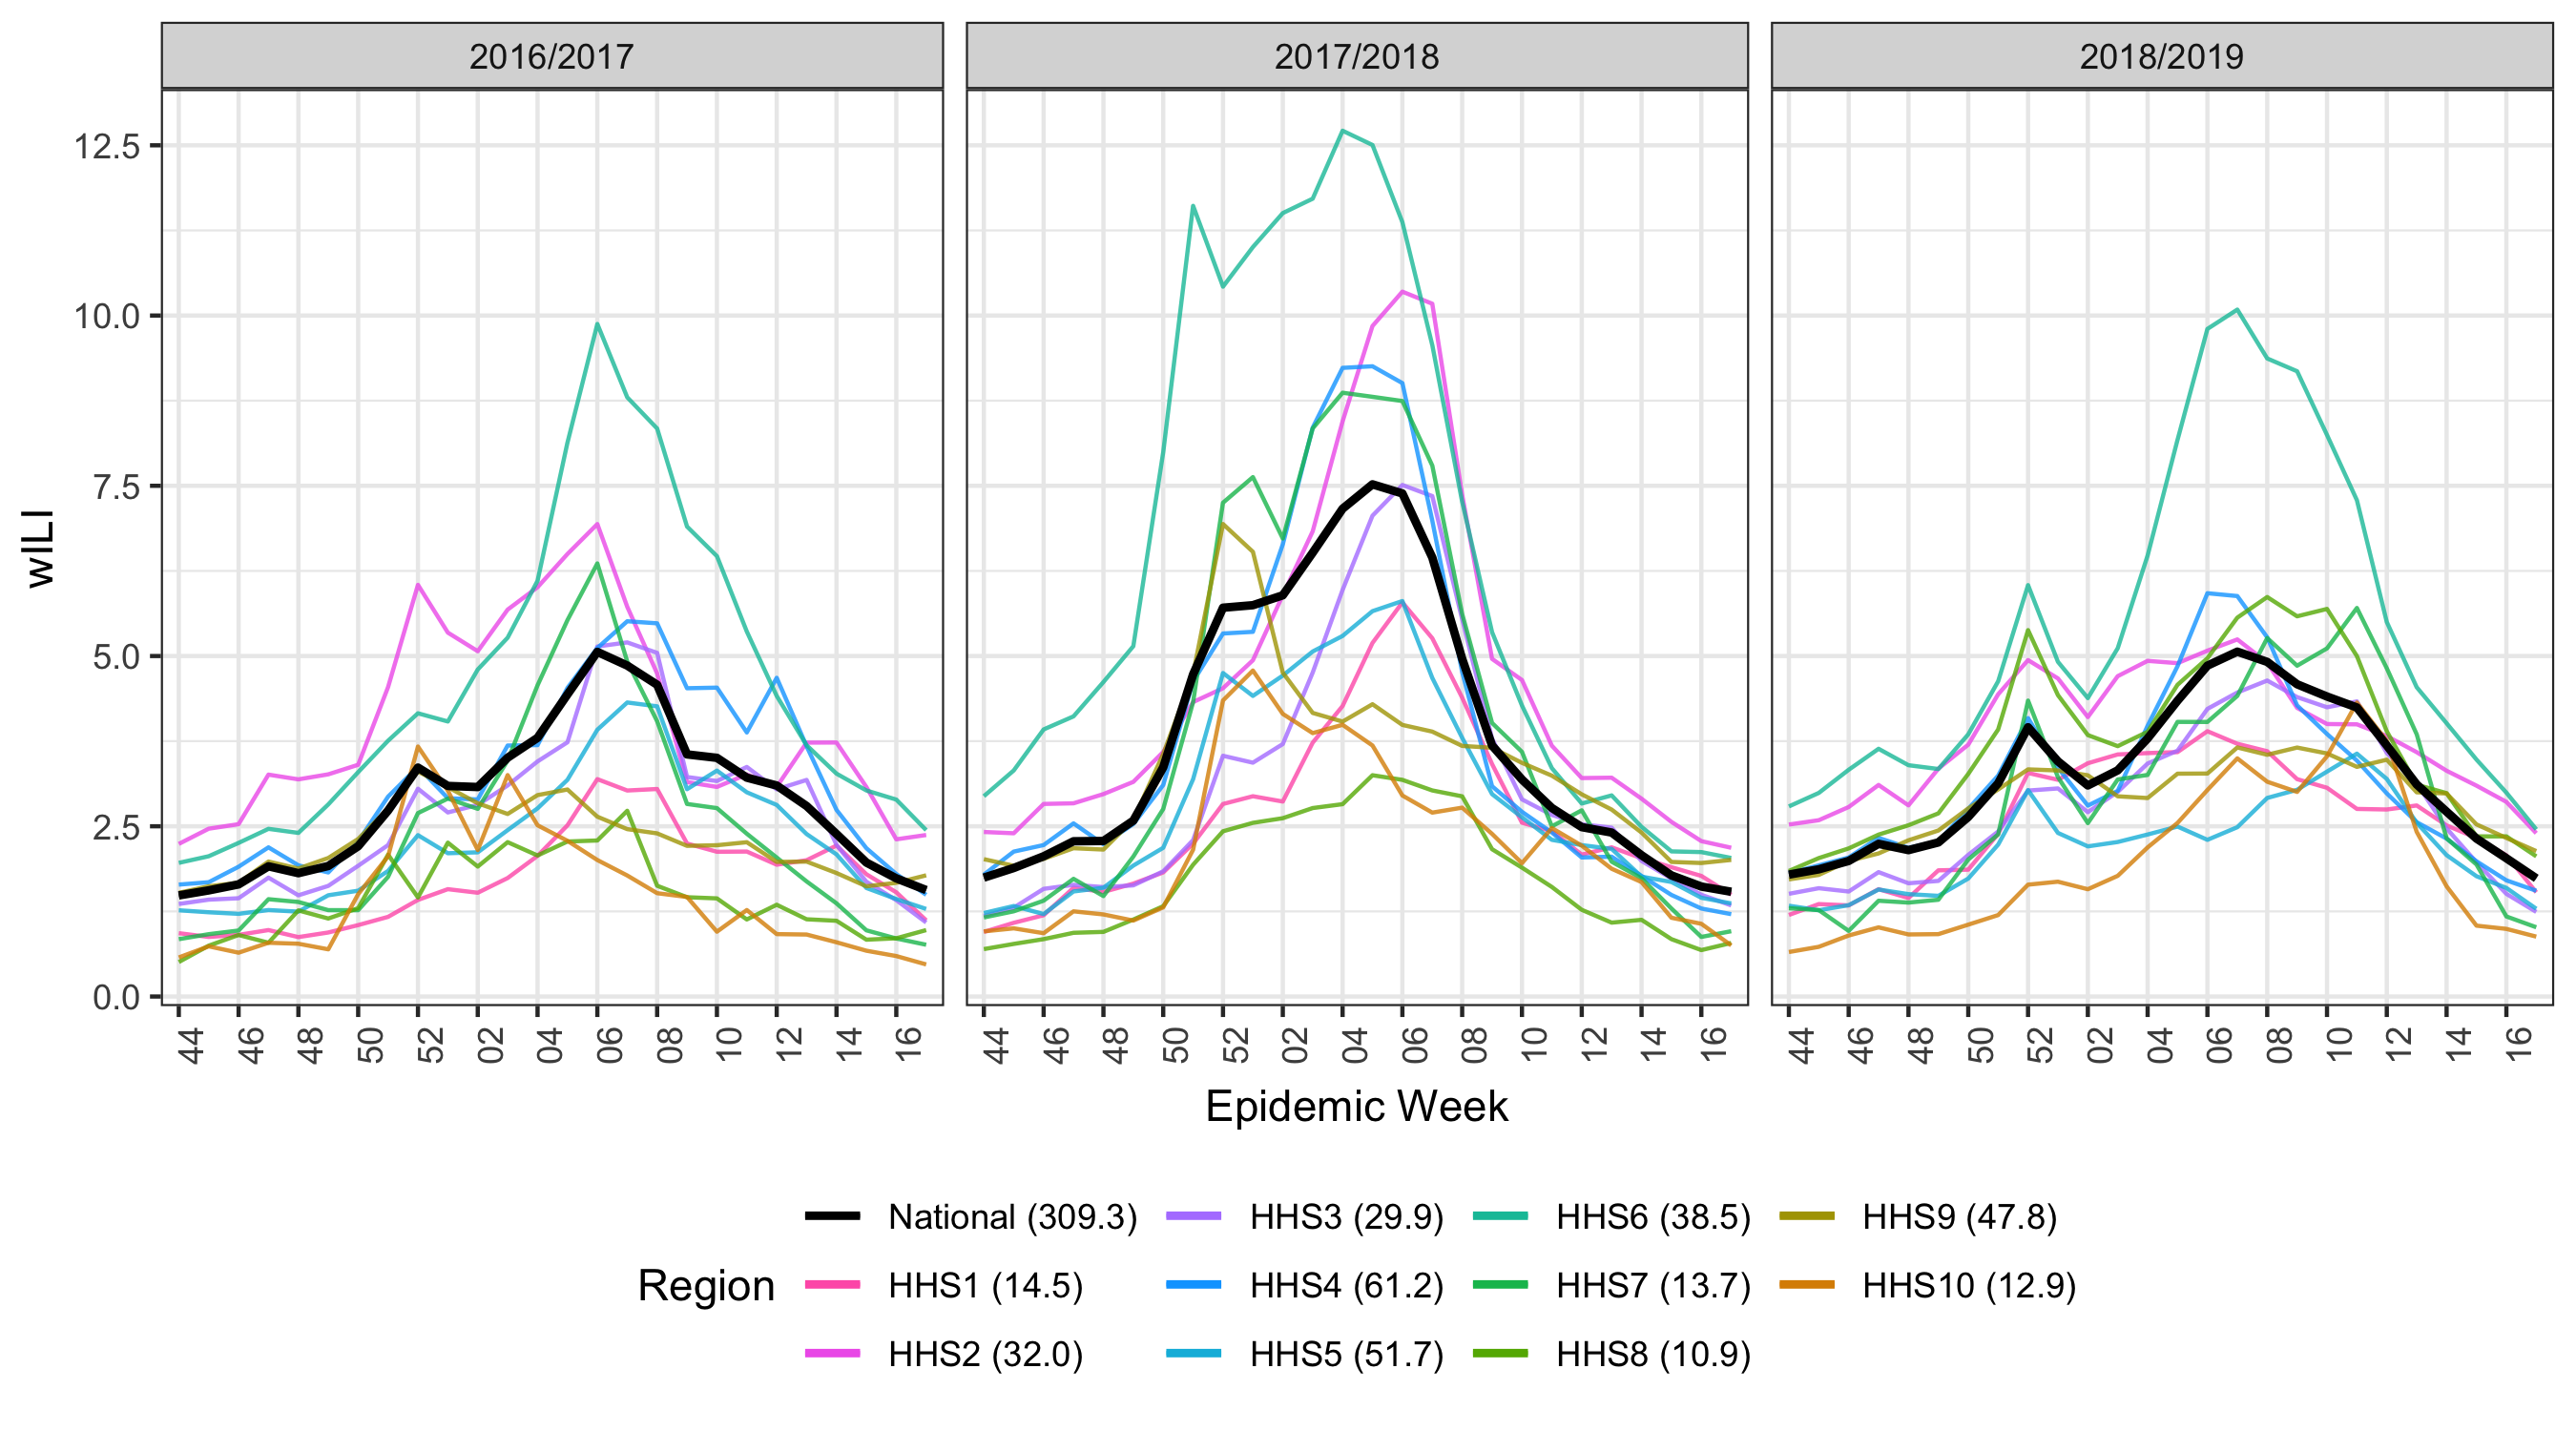
\includegraphics[scale=.2]{data_fig.png}
\caption{Data example for the three test seasons under consideration (2016/2017, 2017/2018, 2018/2019) season for all 10 Health and Human Services (HHS) regions and the national level. At any given epiweek, the national wILI (black) is a weighted sum of regional wILI, where the weights correspond to the population size of the region. We can see that wILI is highly seasonal and varies heavily by region. Region population sizes (in millions) are given next to the region in the legend. }
\label{fig:dgp}
\end{figure}

\subsection{Pointwise Forecast Coherence}



\label{sec:coherence}
The partitioning of national data into HHS regions facilitates geographically localized forecasts, augmenting their usability to local public health officials. A consequence of this partitioning, however, is the creation of a hierarchical structure in the forecasting system. Namely, national wILI data is a linear combination of HHS regional wILI data. Region population sizes (in millions) are given next to the region in the legend of Figure \ref{fig:dgp} as reported by the 2010 U.S. Census \cite{census}.  

We notate the true wILI value as $y_{r,s,w} \in [0,100]$, a percentage for region $r$ in flu season $s$ corresponding to epiweek $w$. Throughout the paper, $r=11$ corresponds to the nation, while $r = 1,2,\ldots,10$ corresponds to HHS region $r$. Let $\alpha_r \in [0,1]$ be a weight corresponding to HHS region $r$, proportional to the population of HHS region $r$, such that  $\sum_{r=1}^{10} \alpha_r =1$. The hierarchical nature of the national/regional partitioning of forecasts for any season and epiweek is equivalent to the following constraint:
\begin{align}
y_{11,s,w} &= \sum_{r=1}^{10} \alpha_r y_{r,s,w}.
\end{align}



 For convenience, define the collection of point forecasts for all regions for season $s$ and epiweek $w$ as
\begin{align}
\tilde{\bm{y}}_{s,w}^T &= [\tilde{y}_{1,s,w},\tilde{y}_{2,s,w},...,\tilde{y}_{11,s,w}].
\end{align}
\noindent We say that the forecast $\tilde{\bm{y}}_{s,w}$ is \emph{coherent} if
\begin{align}
\tilde{y}_{11,s,w} &= \sum_{r=1}^{10} \alpha_r \tilde{y}_{r,s,w},
\end{align}
\noindent and $\tilde{\bm{y}}_{s,w}$ is \emph{incoherent} if
\begin{align}
\tilde{y}_{11,s,w} &\neq \sum_{r=1}^{10} \alpha_r \tilde{y}_{r,s,w}.
\end{align}

Though the existence of the hierarchical structure in the wILI forecasting system is know, many FluSight challenge forecasts are made independently. Forecasting at geographic regions independently provides the forecaster more flexibility to cater models to specific regions or avoid modeling correlation between regions explicitly, but leaves the resulting forecasts vulnerable to incoherence as the true coherent data generating process is not respected. In this paper, we use $\bm{\tilde{y}}$ to represent independently generated and (likely) incoherent forecasts and $\bm{\hat{y}}$ to represent coherent forecasts.

For an independently generated set of forecasts $\bm{\tilde{y}}$, the corresponding coherent projection matrix forecast $\bm{\hat{y}}$ is
\begin{align}
\label{eq:projection}
\bm{\hat{y}} &= \bm{X}(\bm{X}^T \bm{V} \bm{X})^{-1}\bm{X}^T \bm{V} \bm{\tilde{y}} = \bm{P}\bm{\tilde{y}},
\end{align}
\noindent where $\bm{X}$ is a design matrix corresponding to the hierarchical relationship of the data generating process and $\bm{V}$ is a weight matrix. Specifically for the FluSight challenge,




\begin{equation}
\bm{X}_{11 \times 10} =  \begin{pmatrix}
\bm{I}_{10 \times 10} \\
\bm{\alpha}_{1 \times 10} \end{pmatrix}
\end{equation}



\begin{equation}
\bm{\alpha} = [\alpha_1,\alpha_2,...,\alpha_{10}]
\end{equation}

\noindent where $\alpha_r$ is the weight for the $r^{th}$ region. We can think of this as a linear regression model with a design matrix $\bm{X}$ that enforces coherence. Therefore, any projection into the column space of $\bm{X}$, must preserve coherence.


A special case of projection matrix forecasting is when the ordinary least squares (OLS) projection matrix is used, produced by setting $\bm{V}$ equal to the identity matrix $\bm{I}$ in Equation \ref{eq:projection}. This special case has the property that the resulting coherent point forecast $\bm{\hat{y}}$ has mean squared error (MSE) no worse than the independently generated forecast $\bm{\tilde{y}}$ \cite{wickramasuriya2015forecasting}. That is, when $\bm{V}=\bm{I}$ in Equation \ref{eq:projection},
\begin{align}
 || \bm{\tilde{y}} - \bm{y}||_2 &\geq || \bm{\hat{y}} - \bm{y}||_2
\end{align}
\noindent for any $\bm{y}$ and $\bm{\tilde{y}}$ (See Appendix for proof).

For illustration and clarity, consider an example with two low level regions (HHS1 and HHS2) and one top level region (Nation). This example is illustrated in Figure \ref{fig:projection}.

   
\begin{figure}
    \centering
    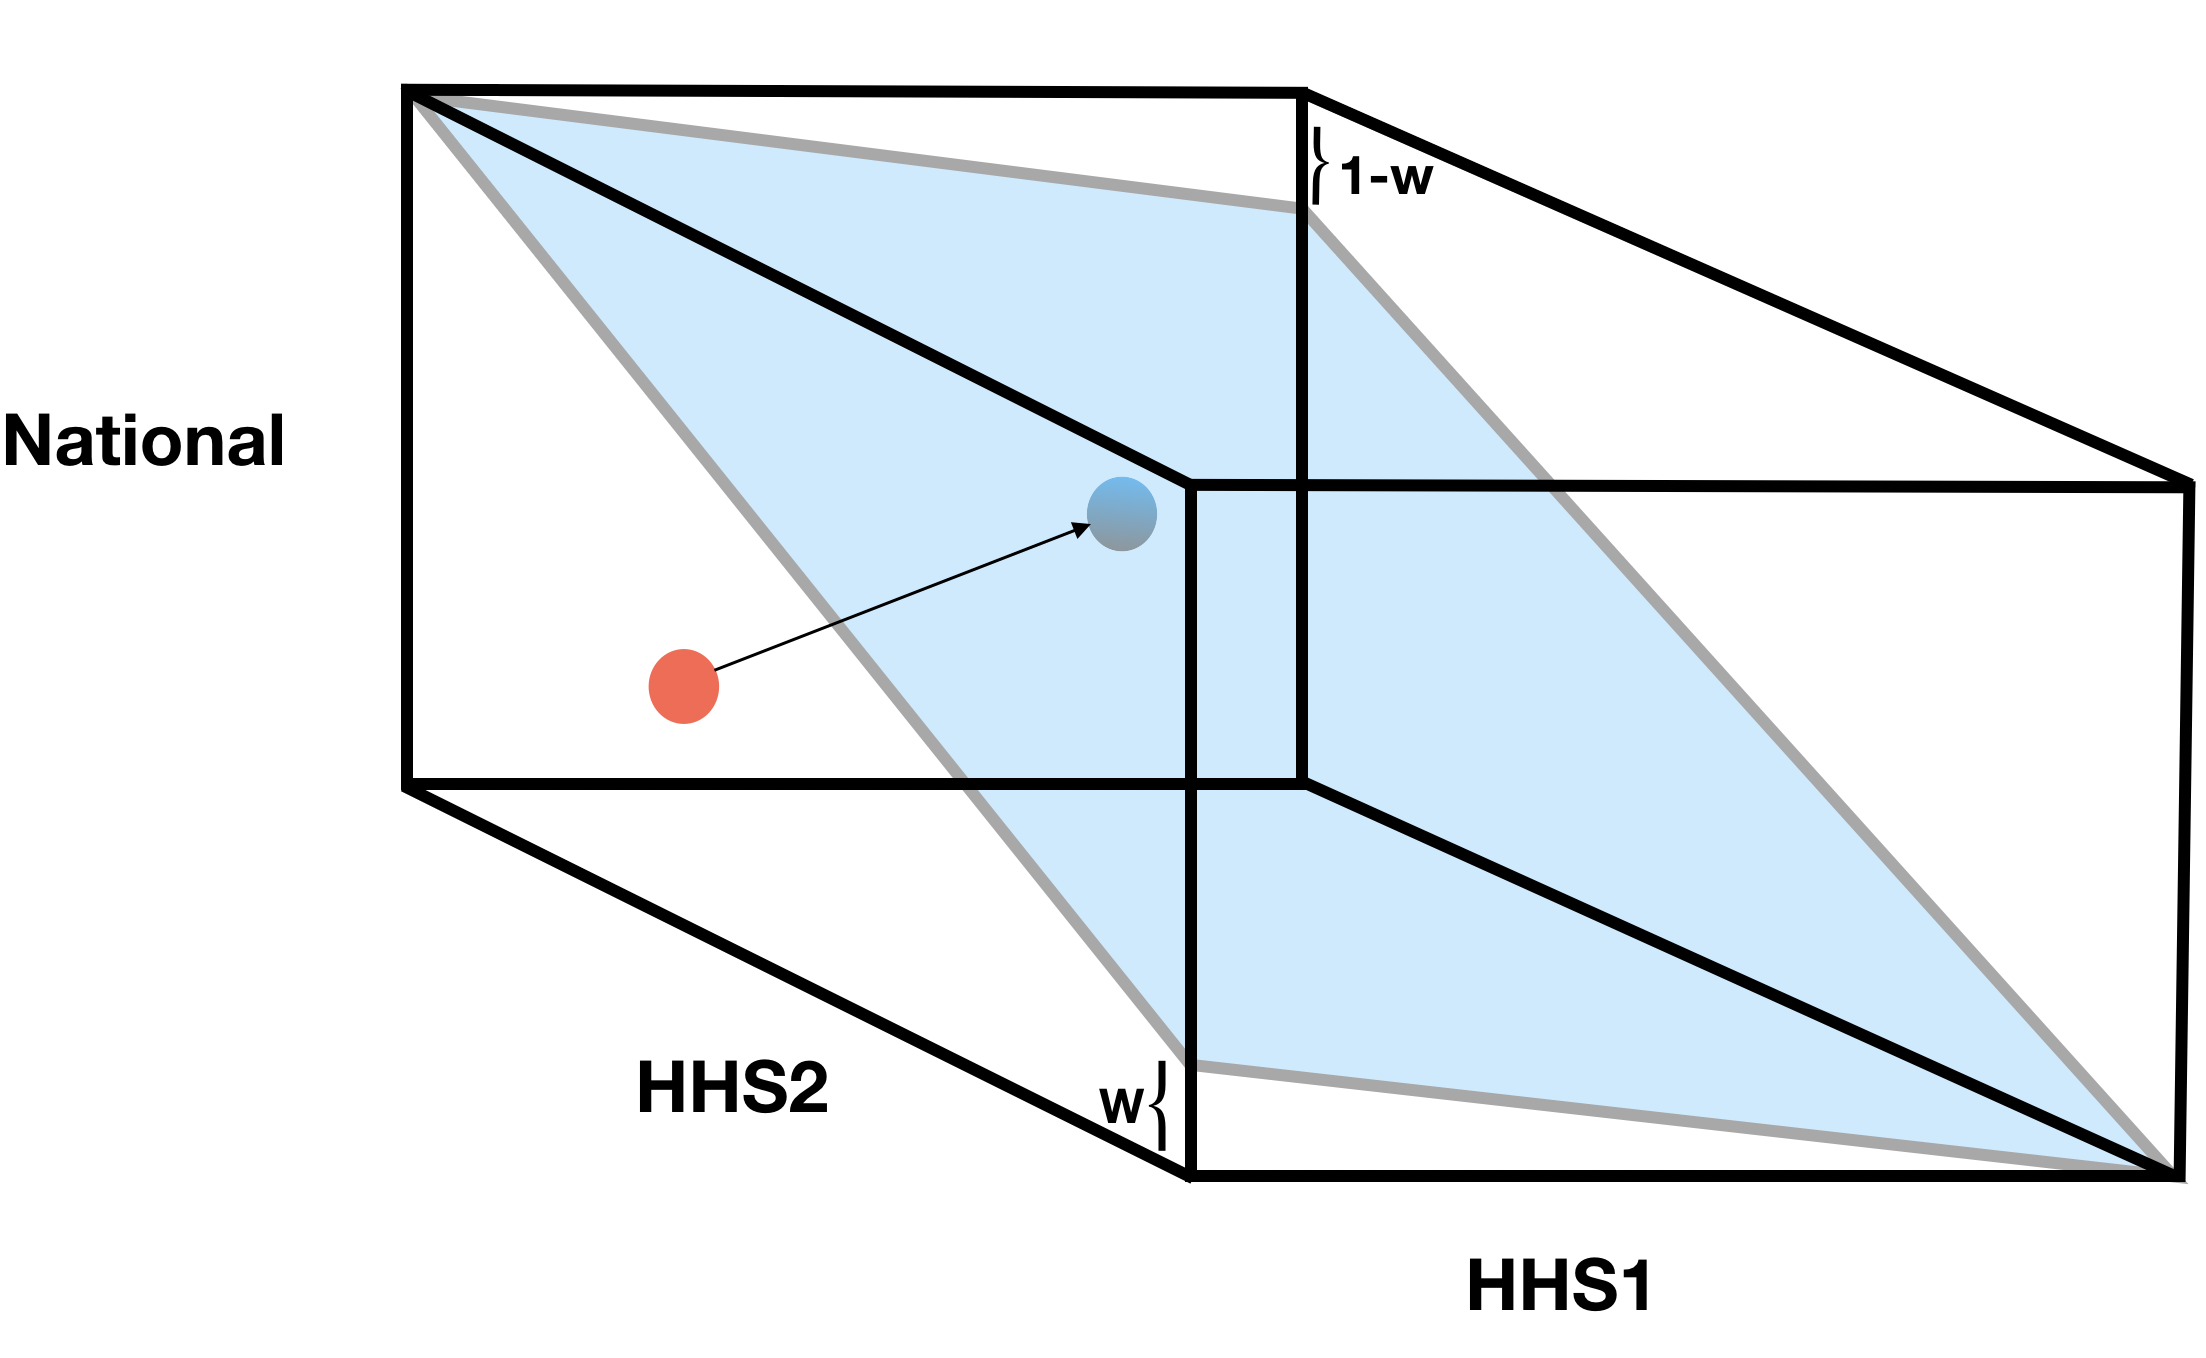
\includegraphics[scale=.25]{projection.png}
    \caption{Mock example of independent forecasts (red) and projected forecasts (blue) for three regions, National, HHS1 and HHS2. Both the blue and the red point represent a triple of ILI forecast values for each region. Independent forecasts are projected onto the space satisfying the constraint of regional level forecasts summing to national level. The blue plane represents the set of points that satisfy the coherence constraint, namely that the weighted combination of region-level forecasts equals the National level forecast. Different projection matrices are able to map the red point to the blue point at different locations on the blue plane. }
    \label{fig:projection}
\end{figure}



Assume
\begin{align}
y_{\text{Nat}} &= \alpha_1 \ y_{\text{HHS1}} + \alpha_2 \ y_{\text{HHS2}},
\end{align}
\noindent where $\alpha_1 = \alpha_2 = 0.5$. Let the true values be
\begin{align}
\bm{y}^T = [y_{\text{HHS1}}, y_{\text{HHS2}} , y_{\text{Nat}}] = [1,1,1],
\end{align}
\noindent and assume the independently generated forecasts are
\begin{align}
\bm{\tilde{y}}^T = [\tilde{y}_{\text{HHS1}},\tilde{y}_{\text{HHS2}},\tilde{y}_{\text{Nat}}] = [1/2, 1/2, 1].
\end{align}
\noindent Notice that the independently generated forecasts are incoherent, as
\begin{align}
\tilde{y}_{\text{Nat}} = 1 & \neq 1/2 =  \alpha_1 \  \tilde{y}_{\text{HHS1}} + \alpha_2 \  \tilde{y}_{\text{HHS2}}.
\end{align}
\noindent The MSE for $\bm{\tilde{y}}$ is
\begin{align}
|| \bm{\tilde{y}} - \bm{y}||_2 &= \frac{1}{3}\Bigg((1/2 - 1)^2 + (1/2 - 1)^2 + (1-1)^2 \Bigg) = 1/6.
\end{align}

The OLS projection matrix forecast is $\bm{\hat{y}} = [2/3, 2/3, 2/3]$, computed as
\begin{align}
\bm{\hat{y}} &= \bm{X}(\bm{X}^T\bm{X})^{-1}\bm{X}^T\bm{\tilde{y}},
\end{align}
\noindent where $$\bm{X} = \begin{pmatrix} 1 & 0 \\ 0 & 1\\1/2 & 1/2 \end{pmatrix}.$$ The projection matrix forecast $\bm{\hat{y}}$ is, by construction, coherent. The effect of the projection matrix forecast is a reduction in MSE over $\bm{\tilde{y}}$, where the MSE for $\bm{\hat{y}} $ is
\begin{align}
|| \bm{\hat{y}} - \bm{y}||_2 &= \frac{1}{3}\Bigg((2/3 - 1)^2 + (2/3 - 1)^2 + (2/3-1)^2 \Bigg) = 1/9.
\end{align}

Note the MSE for $\hat{y}_{\text{HHS1}}$ and $\hat{y}_{\text{HHS2}}$ improved relative to $\tilde{y}_{\text{HHS1}}$ and $\tilde{y}_{\text{HHS2}}$, respectively, while the MSE for $\hat{y}_{\text{Nat}}$ got worse relative to $\tilde{y}_{\text{Nat}}$, resulting in an overall, but not uniform, improvement in MSE for $\hat{\bm{y}}$ relative to $\tilde{\bm{y}}$. The projection matrix forecast is a useful tool for transforming independently generated, incoherent forecasts into coherent forecasts. When $\bm{V}=\bm{I}$ in Equation \ref{eq:projection}, the MSE of the resulting $\bm{\hat{y}}$ is guaranteed to be no greater than the MSE of $\bm{\tilde{y}}$. When $\bm{V} \neq \bm{I}$ in Equation \ref{eq:projection}, the resulting forecast is still coherent, but no such guarantee of MSE improvement exists.
   
   



\subsection{The FluSight Forecast Coherence Dilemma}
   
 Unlike the situations demonstrated in the point forecasting literature, forecasts for the FluSight challenge are required to be probabilistic, not point estimates, and the probabilistic forecasts are evaluated using a multi-bin scoring rule, not MSE. In practice, probabilistic forecasts are generated as a collection of $n$ forecast samples for $y_{r,s,w}$. In this paper, we use the index $i = 1,2,\ldots,n$ to denote draw $i$ from the forecast distribution, resulting in a collection of realizations $\tilde{y}_{r,s,w,i}$. In probabilistic settings we can no longer rely on the coherence definition given in Equation 3. Although various definitions for probabilistic coherence exist \cite{prob_coherence}\cite{taieb2017coherent}, in this paper, we choose the intuitive presentation of Gamakumara et. al \cite{prob_coherence}. We say that the density $f(\tilde{\bm{y}}_{s,w})$ is \emph{probabilistically coherent} if
\begin{align}
f(\bm{\tilde{y}}_{s,w}) &=  0 \  \ \text{when} \  \  \tilde{y}_{11,s,w} \neq \sum_{r=1}^{10} \alpha_r \tilde{y}_{r,s,w}.
\end{align}Here $f$ represents the joint density over all regions and the national level of the hierarchy. Note the close correspondence with the point forecast definition. However, probabilistic coherence does require specification of a joint distribution over regions. Intuitively, this definition says that any point in the support of $f$ that does not obey point-wise coherence is assigned zero probability, (i.e., has measure zero).

Probabilistic forecasts are binned into discrete distributions, where each bin represents a specific wILI level rounded to nearest first decimal. The FluSight challenge uses bins from $\{0.0,0.1,0.2,...,13.0,100\}$ to score discrete probabilistic forecasts. We score forecasts using both ``single-bin skill" and ``multibin-bin skill" \cite{bracher2019multibin} \cite{reich2019reply}. We do this to demonstrate the method's utility on the historical multi-bin skill, as well as the newly adopted single-bin skill. However, unlike the ``log score" (the logarithm of forecast skill) used in the CDC FluSight challenge, we exponentiate the logarithm so that skills remain on the interpretable [0,1] probability scale. Like log score, skill is a thresholding scoring rule, where a forecast is deemed correct if it is within a certain distance of the truth. For single-bin scoring, the probability assigned to the true target $Z_t$ (e.g., a one-week-ahead forecast) corresponding to region $r$ in flu season $s$ and epiweek $w$ under single-bin is computed as
\begin{align}
p_{r,s,w,Z_t} &= \frac{1}{n} \sum_{i=1}^n \bm{1}(\tilde{y}_{r,s,w,i} \in  Z_t),
\end{align}
\noindent where $Z_t$ is the true target. 

We can extend this to multi-bin as 

\begin{align}
p_{r,s,w,Z_t} &= \frac{1}{n} \sum_{i=1}^n \bm{1}(\tilde{y}_{r,s,w,i} \in B),
\end{align}
\noindent where $B = [Z_t - b, Z_t + b]$ for the true target $Z_t$ and some pre-defined threshold $b$. Using a thresholding evaluation metric breaks the guaranteed equal or improved performance of the coherent forecasts when evaluated with MSE.




To see why, consider again the example from Section \ref{sec:coherence} with $\bm{y}^T = [1,1,1]$. For $i=1,2,\ldots,n=10000$, we independently draw
\begin{align}
\tilde{y}_{\text{HHS1},i} &\sim \text{N}(0.5, 0.05),\\
\tilde{y}_{\text{HHS2},i} &\sim \text{N}(0.5, 0.05),\\
\tilde{y}_{\text{Nat},i} &\sim \text{N}(1, 0.05),
\end{align}
\noindent defining $\bm{\tilde{y}}_i^T = [\tilde{y}_{\text{HHS1},i}, \tilde{y}_{\text{HHS2},i}, \tilde{y}_{\text{Nat},i}]$ and $\bm{\hat{y}}_i^T = \bm{X}(\bm{X}^T\bm{X})^{-1}\bm{X}\bm{\tilde{y}}_i$. Figure \ref{fig:my_label} shows the $n$ draws of $\bm{\tilde{y}}$ and $\bm{\hat{y}}$. The single-bin skill counts all forecasts that equal the true value (rounded to the first decimal place) as correct. For every realization $i$, the MSE for $\bm{\hat{y}}_i$ is less than the MSE of $\bm{\tilde{y}}_i$. However, the single-bin skill for the coherent forecasts is 0 while the skill for incoherent forecasts is 0.32 and the skill for the incoherent forecasts is always better than or equal to the skill for the coherent forecasts. This is because all of the national forecasts that fell on top of the truth are projected out of the true bin while the incorrect regional forecasts are moved closer to the correct region, but not close enough to fall inside it. The result is a collection of coherent forecasts with better (lower) MSE, but also lower forecast skill than the incoherent forecasts.

\begin{figure}
       \begin{subfigure}{.5\textwidth}
  \centering
    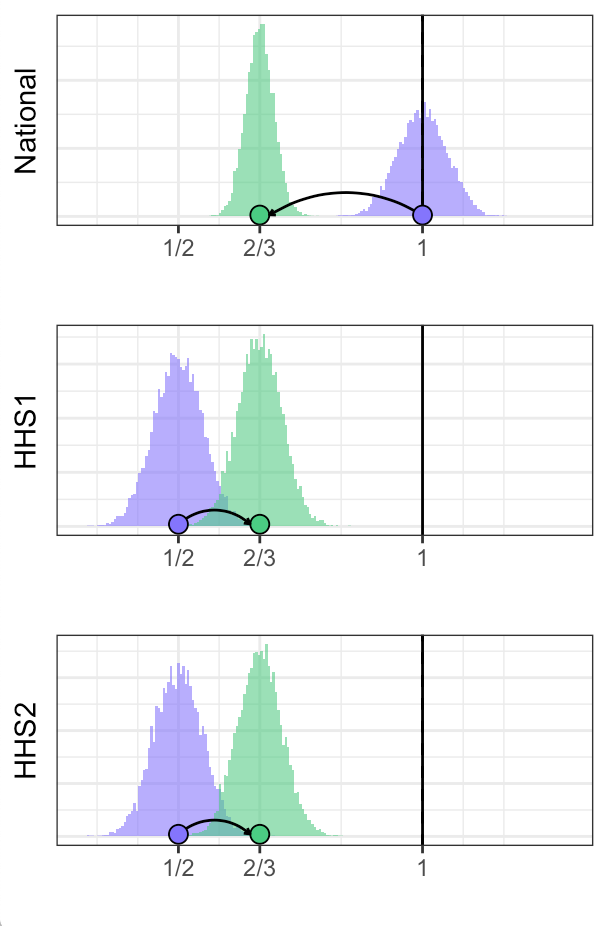
\includegraphics[scale=.6]{cmse_ex2.png}
    \caption{}
\end{subfigure}%
\begin{subfigure}{.5\textwidth}
  \centering
    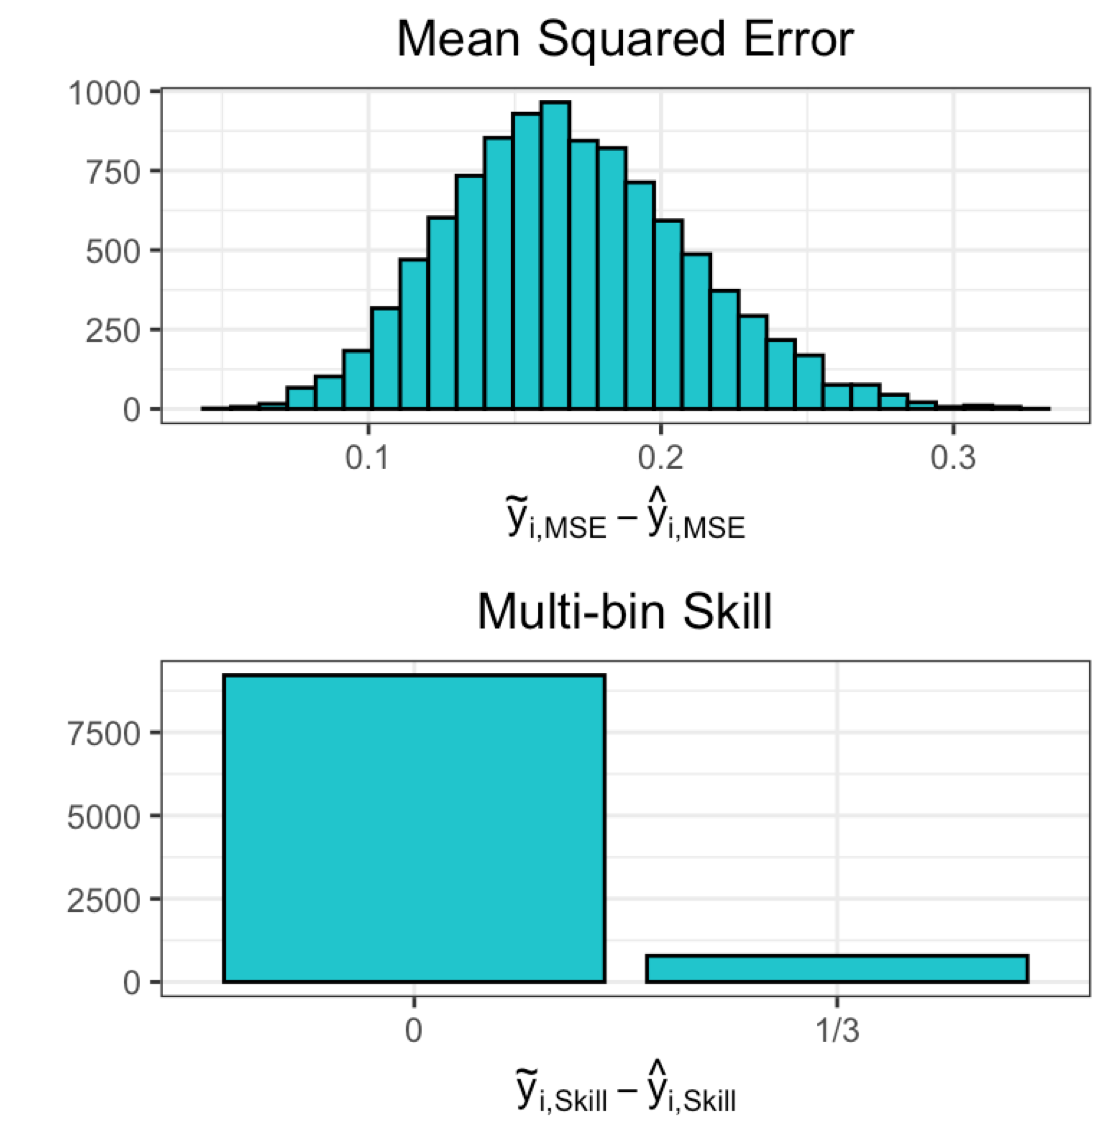
\includegraphics[scale=.4]{cmse_ex1.png}
    \caption{}
\end{subfigure}%

    \caption{Graphical example of how mean squared error (MSE) can decrease while skill gets worse for two region example. \textbf{A:} Purple histograms represent the 10,000 realizations of $\bm{\tilde{y}}$, while green histograms are the corresponding $\bm{\hat{y}}$s. The purple and green points illustrate a particular example of the projection matrix forecasting process. The solid vertical lines denote the true value for each region. \textbf{B:} Top panel shows distribution of MSE for $\bm{\tilde{y}}$ minus corresponding MSE for $\bm{\hat{y}}$. MSE for $\bm{\tilde{y}}$ is greater than the MSE for $\bm{\hat{y}}$ for all realizations. \textbf{B:} Bottom panel shows single-bin skill score for $\bm{\tilde{y}}$ minus skill score for $\bm{\hat{y}}$. The incoherent $\bm{\tilde{y}}$ forecasts are better or equal to the skill for the coherent forecasts for all iterations, with an average improvement greater than 0. This shows the the MSE of the coherent forecasts has decreased (since the difference between the original and projected is positive) and the forecast skill has decreased (since the difference between the original and projected is again positive). Since a decrease in MSE means an improvement and a decrease in forecast skill means a lack of improvement, we see that coherence can have opposite effects on the two scores.  }
    \label{fig:my_label}
\end{figure}


\subsection{Problem Statement}
 
 On one hand, we have a guarantee that the MSE of point forecasts projected into the data generating process space can get no worse under the OLS projection method. On the other, we have an explicit example of forecast skill decreasing as a result of forecasts projected into the data generating process space. This seeming inconsistency leads us to the central question of this paper: Can probabilistic forecast coherence be used to improve forecast skill when forecasting influenza? The remainder of this paper will investigate this question. In this analysis, we focus only on short-term (1-4 week ahead) targets. The definition of coherence is less clear on seasonal targets, since knowing the regional season peaks does not inform the national season peak. 


\section{Methods}



In order to investigate the question posed in Section 1.4 we developed four methods to sample from probabilistically coherent forecast densities. To begin, we define the joint density of original forecast densities, drawn independently for each region:

\begin{equation}
f(\tilde{\bm{y}}) = \prod_{r=1}^{11} f_r(\tilde{y}_r).
\end{equation}

\noindent Previous approaches have factored $f(\tilde{\bm{y}})$ into a bottom-up density, where

\begin{equation}
f(\tilde{\bm{y}}) = \delta(\tilde{y}_{11} | \tilde{y}_{1:10})h(\tilde{y}_{1:10} | \theta),
\end{equation}
where $\delta$ is a Dirac delta density centered at  $\tilde{y}_{11} = \sum_{r=1}^{10} \alpha_r \tilde{y}_r$, $\theta$ is a parameter(s) estimated from training data, and $h$ is a joint density over all 10 regions \cite{taieb2017coherent}.



The bottom-up model of Equation 23, while probabilistically coherent, lacks robustness in two key ways. First, it requires historical training data to estimate $\theta$. This is not always possible, particularly in emerging epidemic settings. Second, the bottom-up approach ignores information encoded in the original forecast density for the national region $\tilde{y}_{11}$.  We instead develop methods that take draws from $f(\tilde{\bm{y}})$ of Equation 23 and produce draws for a probabilistically coherent $f^*(\hat{\bm{y}})$. These methods address both of the shortcomings of the bottom-up density of Equation 23: they do not discard national scale forecasts and they do not require training data.





\begin{figure}
    \centering
    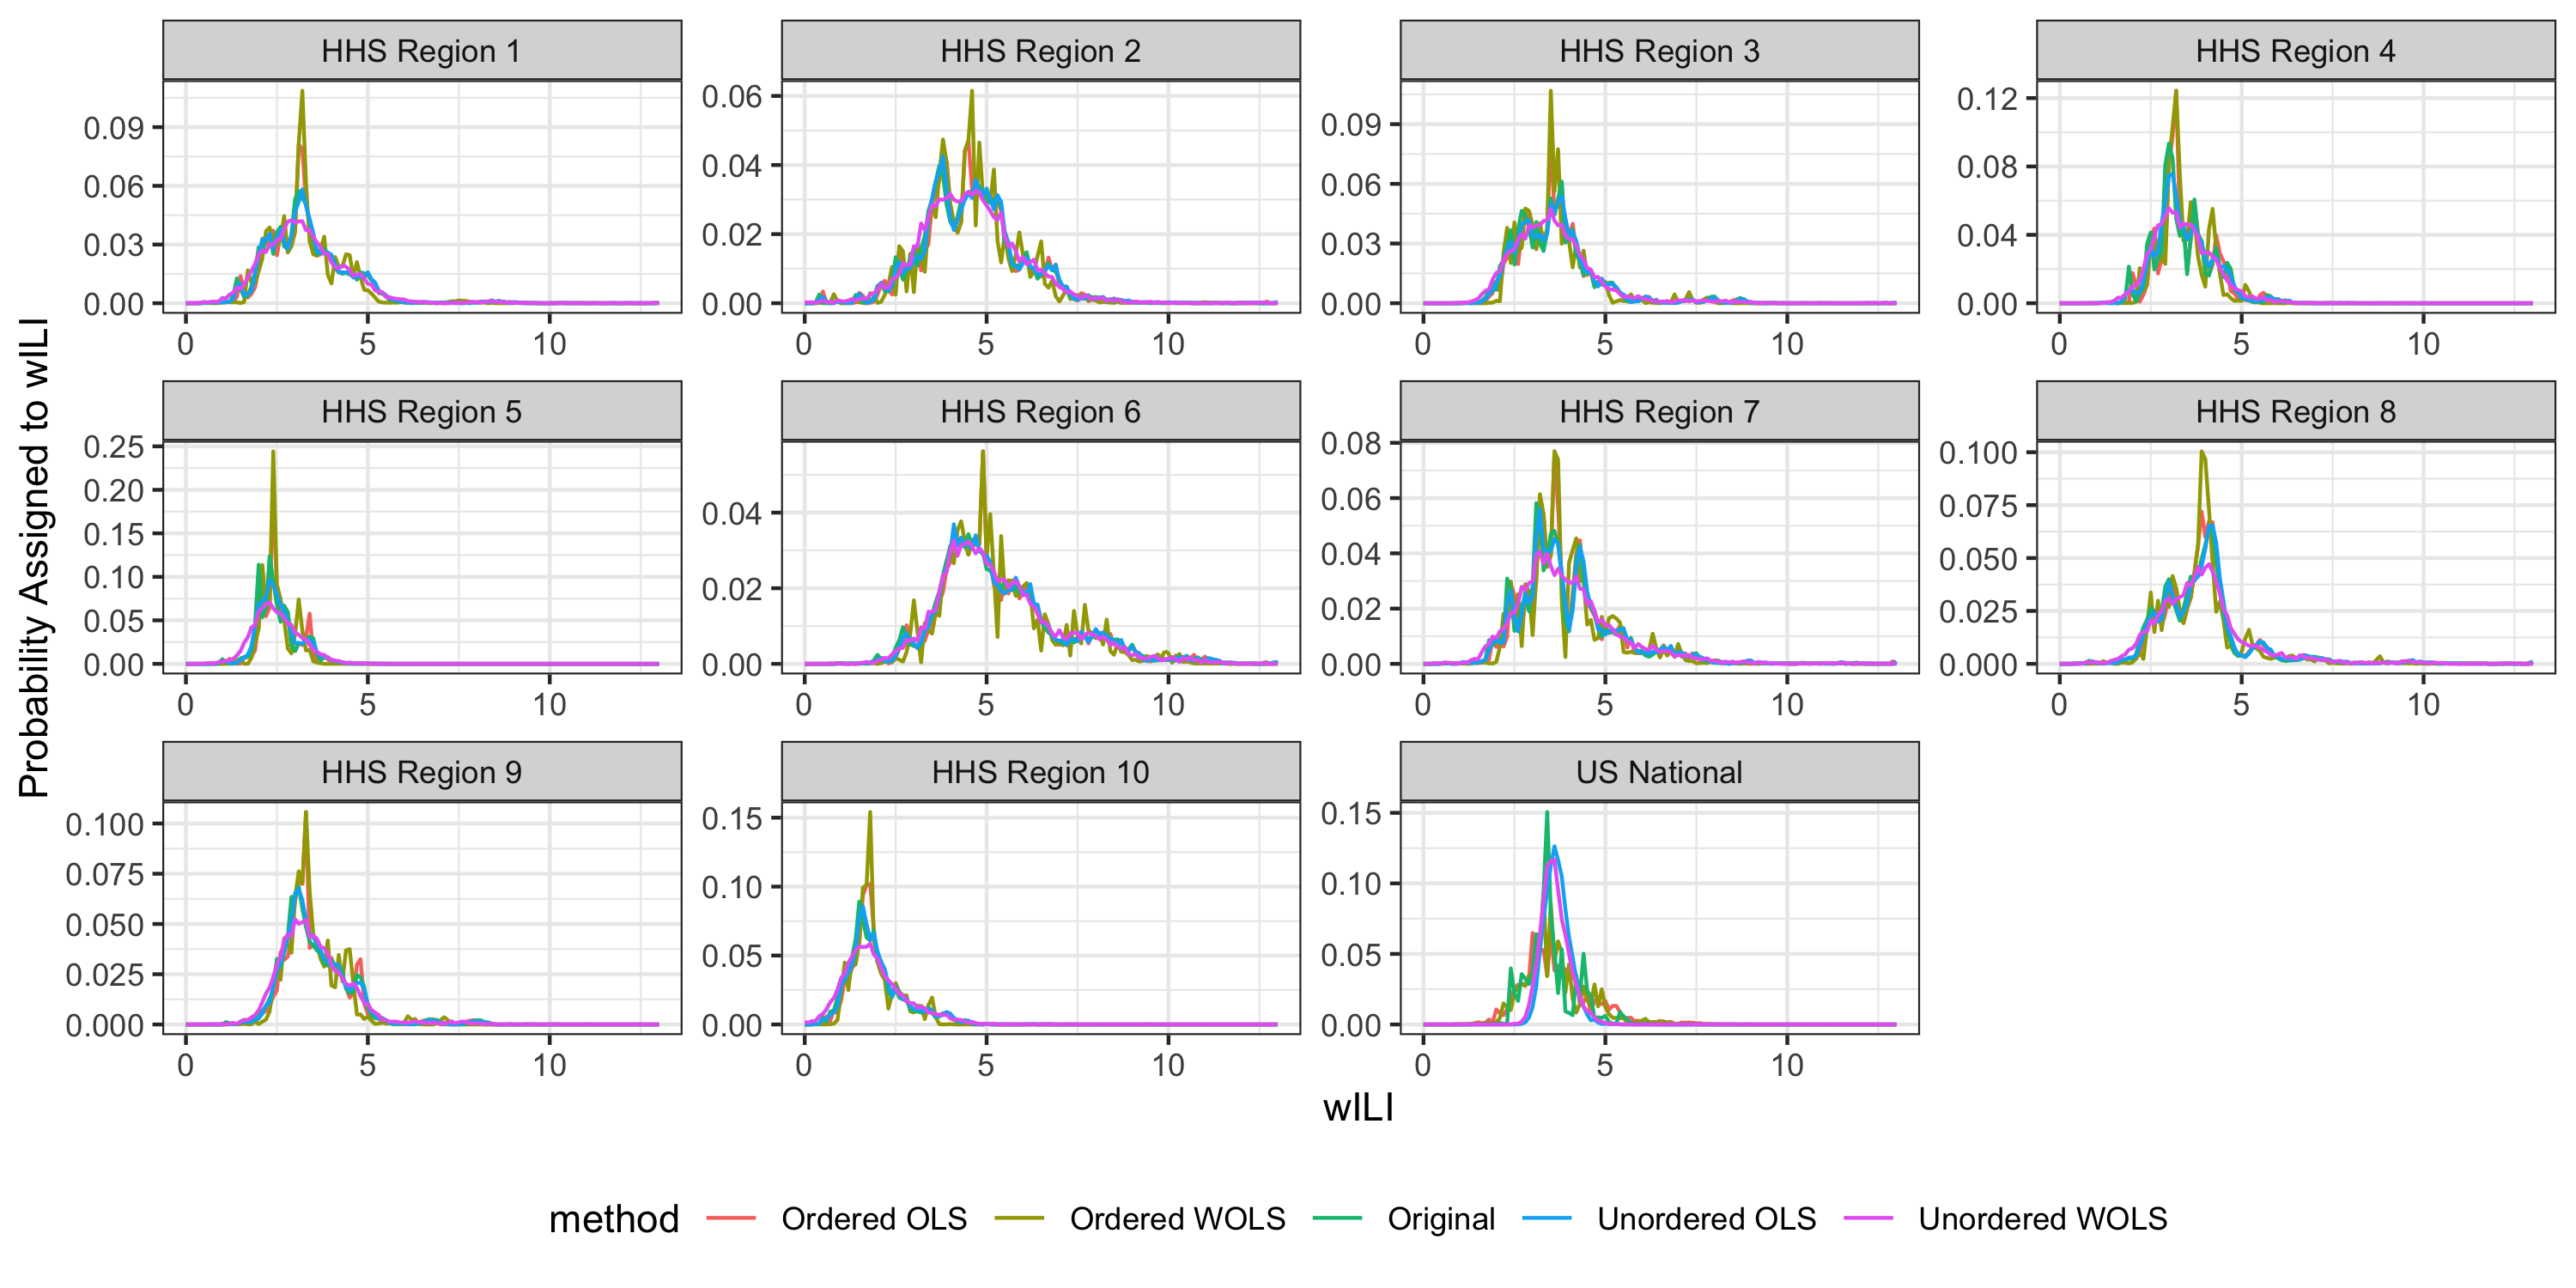
\includegraphics[scale=.175]{fig_5.png}
    \caption{ Real data example of model predictive densities for the 1 week ahead target on epiweek 201901 for the 2018/2019 season across all 11 regions. The y-axis represents the probability density for a given wILI bin value on the x-axis. Notice how the regional samples do not change much under the coherence constraint, but the national forecasts noticeably change. We can also see variable levels of density ``smoothing" produced by each method, with the greatest amount of smoothing under the Unordered weighted ordinary least squares (WOLS) method. This smoothing of forecast density also lowers the magnitude of the peak density across all HHS regions, but increases the magnitude of the peak in the nation. However, the overall location of the forecast density remains consistent across all projection methods.  }
    \label{fig:pcc_example}
\end{figure}




In what follows we consider four projection approaches for sampling from the probabilistic coherent density, $f^*(\hat{\bm{y}})$, as well as two baseline approaches. We first consider the scenario where forecast distributions are assumed to be uncorrelated across regions and where forecasts from each region are weighted equally. This allows us to sample from the original forecast distribution $f(\tilde{\bm{y}})$ and apply a point-wise coherence projection matrix to each independently drawn sample $\tilde{\bm{y}_i}$. In the second approach, we assume the geographical units are positively correlated and forecasts from each region are weighted equally. This correlation structure reflects our knowledge that during an epidemic, forecast models that tend to under predict wILI at the regional level, will also do so at the national level. The correlation induced creates a positive correlation between all the regions and the nation. Third, we consider the case where regions are uncorrelated but we allow forecasts for regions with larger populations to be weighted more heavily than those with smaller populations. This allows us weight forecasts made from regions with larger populations (i.e. larger sample sizes) more heavily in the projection. Fourth, we consider forecasts as both correlated across regions and variable according to population of the region. Finally, we include the original forecast distribution and the bottom-up method as reference models. 


\subsection{ Ordinary Least Squares}

Our first approach requires samples from the independent forecast distributions, defined as follows:

\begin{equation}
\tilde{y}_{1,i} \sim f_1(\tilde{y}_1), \  \ \tilde{y}_{2,i} \sim f_2(\tilde{y}_2), \  \ ... \ , \ \ \tilde{y}_{11,i} \sim f_{11}(\tilde{y}_{11}),
\end{equation}where $i$ indexes samples and where we have dropped the season, epiweek, and model index for simplicity. We then apply the projection matrix to the column vector

\begin{equation}
\bm{\hat{y}}_i=\bm{P} \begin{pmatrix} \tilde{y}_{1,i} \\ \tilde{y}_{2,i} \\ ... \\ \tilde{y}_{11,i} \end{pmatrix} \ \ = \bm{P}\bm{\tilde{y}}_i.
\end{equation}This approach is graphically demonstrated in Figure \ref{fig:projection}. Using the projection matrix on each sample guarantees that the resulting empirical probability mass function satisfies the probabilistic coherence definition of Equation 16. Algorithm 1 outlines how to produce samples from $f^*(\hat{\bm{y}})$. In practice, the CDC submission files specify probability distributions as binned probability mass functions. Independent forecasts $\boldsymbol{\tilde{y}}_i$ are sampled from these binned probability mass functions.

\begin{center}
\begin{algorithm}
    \begin{algorithmic}[1]
        \For{r = 1,2,...,11}
\For{ i = 1,2,....,n}
\State $\tilde{y}_{r,i} \sim f_r$
\EndFor
\EndFor
\For{ i = 1,2,....,n}
\State $\hat{\bm{y}}_{i} = \bm{P} \tilde{\bm{y}}_{i} = \bm{P} \begin{pmatrix} \tilde{y}_{1,i} \\ \tilde{y}_{2,i} \\ ... \\ \tilde{y}_{11,i}  \end{pmatrix}$
\EndFor

    \end{algorithmic}
    \label{alg:rAP}
    \caption{Unordered OLS sampling from probabilistically coherent joint distribution given a collection of marginal distributions. Note that the corresponding weighted ordinary least squares (WOLS) method is obtained by replacing $\bm{P}$ with $\bm{P}_w$.}
\end{algorithm}
\end{center}


\subsection{Ordered Ordinary Least Squares}

The unordered OLS approach assumes no correlation between the error structures regionally and nationally. That is, each sample is generated independently. In the second approach we induce a correlation structure between the forecast distributions. We begin with the same set of samples as defined in Equation 22. However, before applying the projection matrix we first compute the order statistics.  We then apply the projection matrix to the column vector of the aligned order statistics:

$$\bm{\hat{y}}_{i}=\bm{P} \begin{pmatrix} \tilde{y}_{1_{(i)}} \\  \tilde{y}_{2_{(i)}} \\ ... \\  \tilde{y}_{11_{(i)}} \end{pmatrix} = \bm{P} \bm{\tilde{y}}_{(i)}$$

\noindent where $\tilde{y}_{r_{(i)}} $ is the $i^{th}$ order statistic for the empirical distribution $f_r(\tilde{y}_{r})$ for region $r$.

Both the ordered and unordered OLS approaches lead to empirical distributions that are probabilistically coherent, however, the ordered OLS approach induces a correlation structure where low regional wILI forecasts  are tied to low national wILI forecasts and vice versa: similar to the Schaake Shuffle \cite{scheffe}. In practice, the ordered OLS algorithm amounts to first sorting the samples drawn independently at each region and then applying the projection matrix to the sorted samples as outlined in Algorithm 2.



\subsection{ Weighted Ordinary Least Squares}

In order to incorporate our uncertainty of the independent forecasts made in each region, we generalize the OLS method to weighted ordinary least squares (WOLS), where the weight matrix $\bm{V}$ is a diagonal matrix with entries corresponding to the inverse of the population weights for the region,

\begin{align}
diag(\bm{V}^{-1}) =\{\alpha_{\text{HHS}1},\alpha_{\text{HHS}2},...,\alpha_{\text{HHS}10},1 \}
\end{align} 

where $\alpha_j$ is the normalized population weight defined in Section 1.2. The projection $\bm{P_{V}}$ matrix becomes,

\begin{align}
\bm{P}_V= \bm{X}(\bm{X}\bm{V}\bm{X^T})^{-1}\bm{X^T}\bm{V}
\end{align} 

The WOLS maintains a coherent projection in that applying $\bm{P}_V$ to a vector projects the vector into the column space of $\bm{X}$, but allows us to treat each forecast with a different degree of certainty. The weighted projection can be extended to allow for correlation using the ordered approach described in Section 2.2, but replacing $\bm{P}$ with $\bm{P}_V$. 





\begin{center}
\begin{algorithm}
    \begin{algorithmic}[1]
        \For{r = 1,2,...,11}
\For{ i = 1,2,....,n}
\State $\tilde{y}_{r,i} \sim f_r$
\EndFor
\EndFor
\For{ i = 1,2,....,n}
\State Set $y_{(i)} $ to the $i^{th}$ order statistics 
\State $\hat{\bm{y}}_{i} = \bm{P}\tilde{\bm{y}}_{(i)} = \bm{P} \begin{pmatrix} \tilde{y}_{1_{(i)}} \\ \tilde{y}_{2_{(i)}} \\ ... \\ \tilde{y}_{11_{(i)}}  \end{pmatrix}$
\EndFor

    \end{algorithmic}
    \label{alg:rAP}
    \caption{ Ordered OLS sampling from probabilistically coherent joint distribution given a collection of marginal distributions. Note that the corresponding WOLS method is obtained by replacing $\bm{P}$ with $\bm{P}_V$.}
\end{algorithm}
\end{center}



\subsection{Ordered Weighted Ordinary Least Squares}

Finally, we can apply the same ordering step to the weighted least squares projection. This requires computing the order statistics and applying the weighted projection matrix ($\bm{P_V}$)
$$\bm{\hat{y}}_{i}=\bm{P}_V \begin{pmatrix} \tilde{y}_{1_{(i)}} \\  \tilde{y}_{2_{(i)}} \\ ... \\  \tilde{y}_{11_{(i)}} \end{pmatrix} = \bm{P}_V \bm{\tilde{y}}_{(i)}$$

This leads to a set of forecasts that are both correlated and weighted by a normalized population measure to reflect our uncertainty of the independent forecasts by region. This method is a composition of Section 2.2 and 2.3.



\subsection{Experimental Setup}

In order to examine the effects of the unordered and ordered OLS/WOLS approaches on forecast skill, we use submission files for the 2016/2017, 2017/2018, and 2018/2019 seasons that have been submitted to the CDC and are uploaded to the central repository \cite{forecasts}. For each evaluation season, we obtain a list of all models submitted, and evaluate all four approaches across both single and multi-bin scoring for 1-4 week ahead targets across epiweeks 44-17. Any model that did not have a complete set of submission files for all 1-4 week ahead targets, all epiweeks, and all regions was discarded.  The sample sizes for the evaluation are included in Table 1, where we define an evaluation point as a unique region, season, model, epiweek, and target combination. As we can see from Table 1, the sample sizes are quite substantial when aggregating over evaluation points. We use the 2010 U.S. Census weights across all seasons as an estimate of $\alpha_r$ for each region \cite{census}. The correlation between the weighted combination of the regionally reported wILI by the CDC and the nationally reported wILI is $>.99$.  Using the 2010 U.S. Census weights is a reasonable approximation to the weights used by the CDC.

\begin{table}[h!]
\caption{Experimental setup for evaluating probabilistic coherence approaches. An evaluation point is defined as a unique region, season, epiweek, target, and model combination.}
\begin{center}
\begin{tabular}{ |c|c|c| }
\hline
 \textbf{Season} & \textbf{Number of Models} & \textbf{Number of Evaluation Points} \\
 \hline
 2016/2017 & 24 & 27,456  \\
 \hline
 2017/2018& 24 & 27,456 \\
 \hline
 2018/2019 & 35 & 40,040 \\
 \hline
\end{tabular}
\end{center}

\end{table}






\section{Results}

	In what follows we consider the combination of a model and a season as the fundamental unit of analysis on which to base our conclusions. As a forecaster, the main question under consideration is whether applying forecast coherence will improve the average forecast skill of a given model in an upcoming season. As we can see from Table 2 the results vary heavily by scoring method used. For the main results, we use single-bin skill as this is the most up to date skill used in the FluSight challenge, but we also present various summary results for multi-bin to highlight the differences in results under different scoring mechanisms. 

Under single-bin scoring we saw 79\% of models improve under the unordered WOLS method, 64\% of models improve with unordered OLS, 51\% of models improve with ordered OLS, and 31\% of models improve with ordered WOLS. As seen in Figure \ref{fig:model_results}, the increase in skill ranged from -.005 to .025 under single-bin with a mean of .002 and variance 1.7e-05. This shows that the magnitude of improvement is greater than the magnitude of decrease. This asymmetry is even more pronounced in the multi-bin scores ( Figure \ref{fig:model_results} right), with the greatest improvement in skill of .15 and biggest loss in skill of -.005. The average increase under multi-bin scoring for the ordered OLS method was .0024 and variance 2.8e-03.  

We can see that 17 model season combinations got worse under unordered WOLS and single-bin scoring and only 5 models got worse under ordered OLS and multi-bin scoring (Figure   \ref{fig:model_results} ).This suggests that modeling the correlation structure has a significant effect on the results under single-bin scoring, with unordered WOLS improving significantly more than ordered WOLS (79\% vs 31 \%).  However, the correlation structure did seem to improve skill under multi-bin scoring, with ordered OLS improving significantly more than unordered OLS (90\% vs 51\%). Further work that allows for assumptions in between these two extremes is required. The results also suggest that the weighting is important under single-bin scoring. 

\begin{table}
\begin{center}
  \begin{tabular}{ | l | c | r |  }
    \hline
   \textbf{Percent of forecasts improved} & \textbf{Single-Bin} & \textbf{Multi-Bin}  \\ \hline
    Unordered OLS & 64 &  65 \\ \hline
    Ordered OLS  &51 & 90  \\ \hline
    Unordered WOLS & 79 & 53   \\ \hline
     Ordered WOLS &  31 & 57  \\ \hline
     Bottom Up  & 39 &  59  \\ \hline
  \end{tabular}
  \end{center}

  \caption{Percent of forecasts improved over original forecast distribution for the four coherence methods described, in addition to the baseline bottom up model under both single-bin and multi-bin skill. We omit the independent forecasts since they are the reference model for percentage of forecasts improved. Notice that WOLS unordered showed the greatest improvement under single-bin scoring but showed the least improvement under multi-bin scoring. This demonstrates that the scoring rule used influences the performance of the coherence methods.  }
\end{table}

  \begin{figure}
   \begin{subfigure}{.5\textwidth}
  \centering
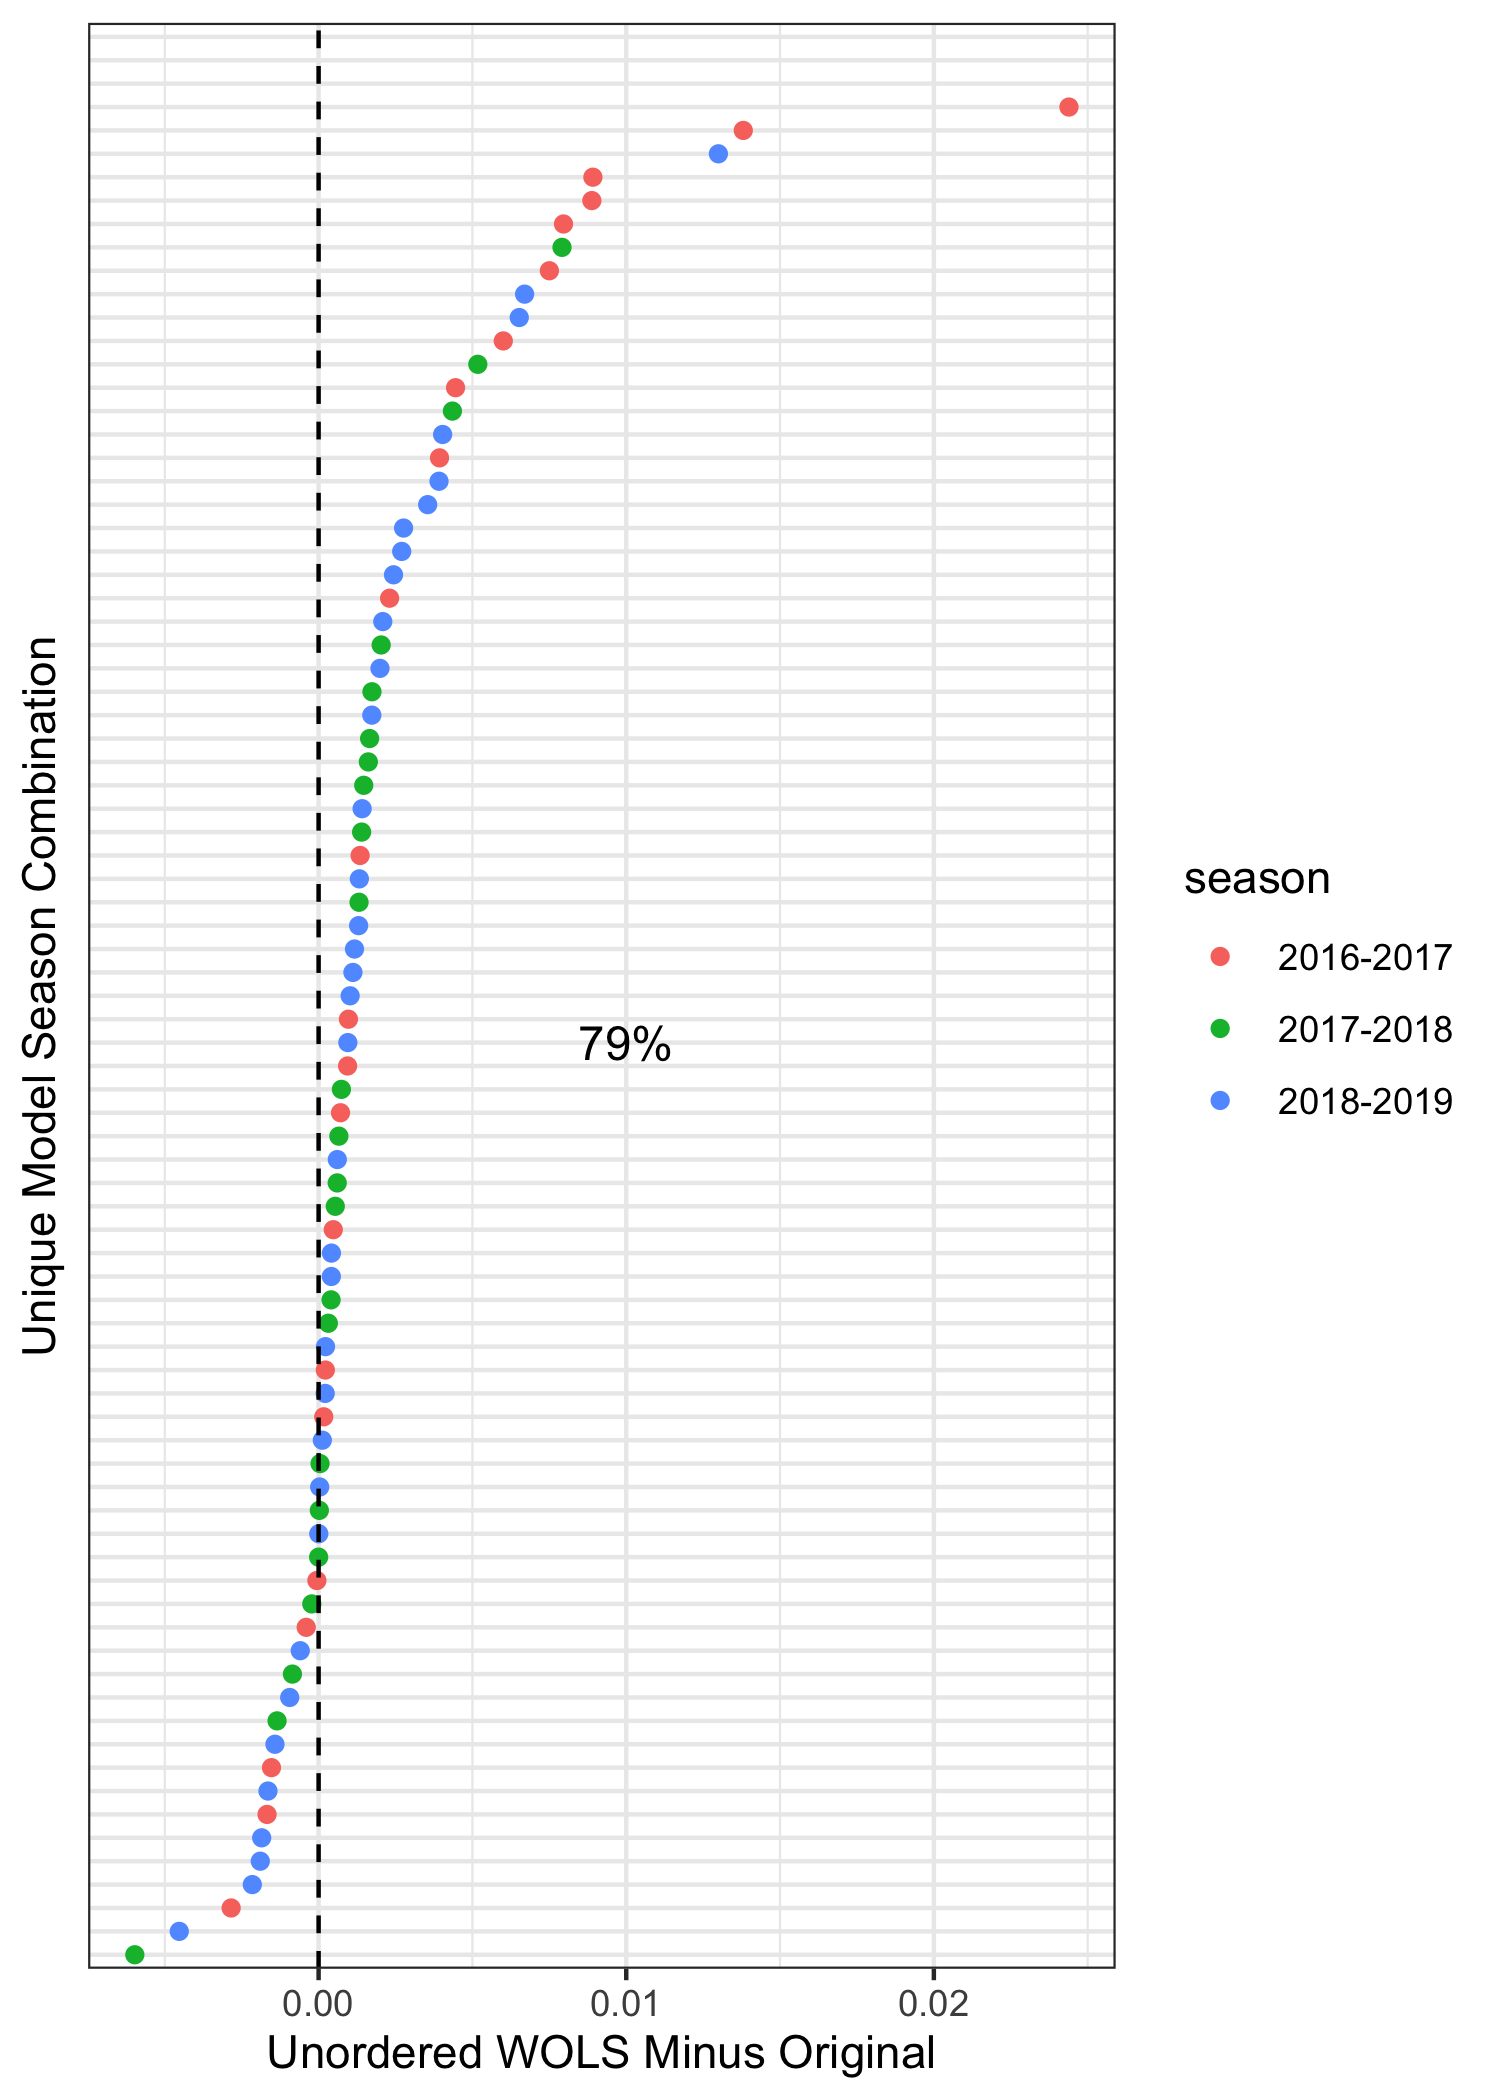
\includegraphics[scale=.15]{single_bin_unordered.png}
 \caption{Unordered WOLS under Single-Bin}
\end{subfigure}%
\begin{subfigure}{.5\textwidth}
  \centering
    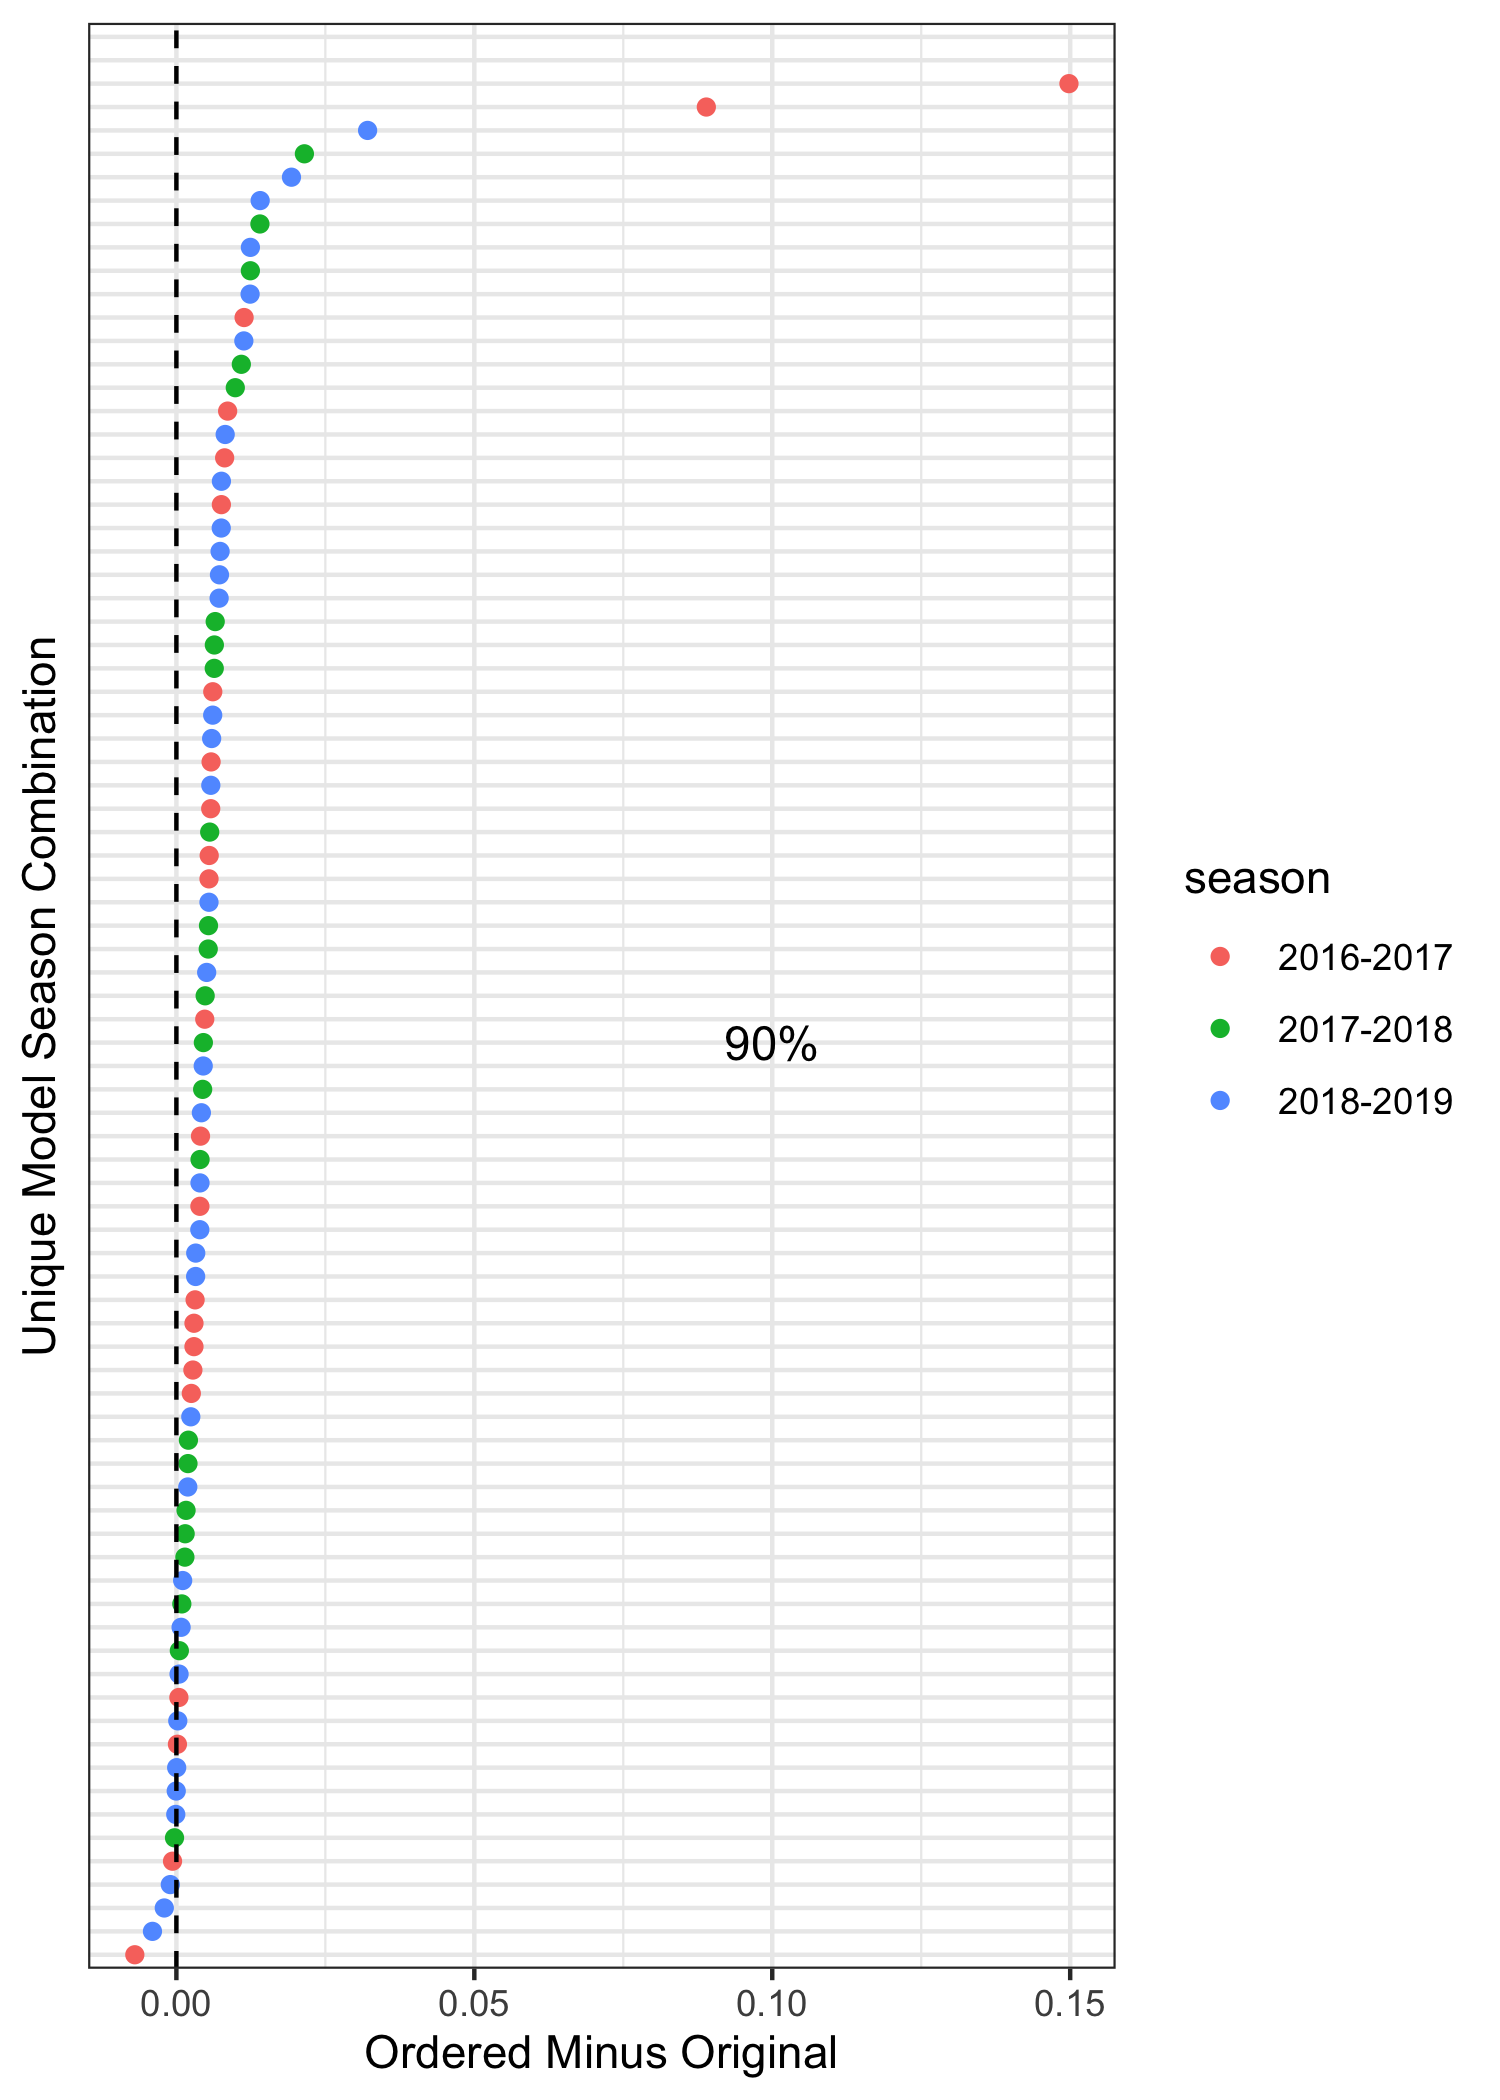
\includegraphics[scale=.15]{multi_bin_ordered.png}
    \caption{Ordered OLS under Multi-Bin}
\end{subfigure}


\caption{Best performing method under single-bin (left) and mutli-bin (right) in terms of forecast skill averaged over all targets (1-4 week ahead), regions (HHS1-10 \& National) and broken down by model-season combination. The y-axis represents a unique season model combination which has been made anonymous to protect participant teams identity. }
\label{fig:model_results}
\end{figure}



     \begin{figure}
   
\begin{subfigure}{.5\textwidth}
  \centering
    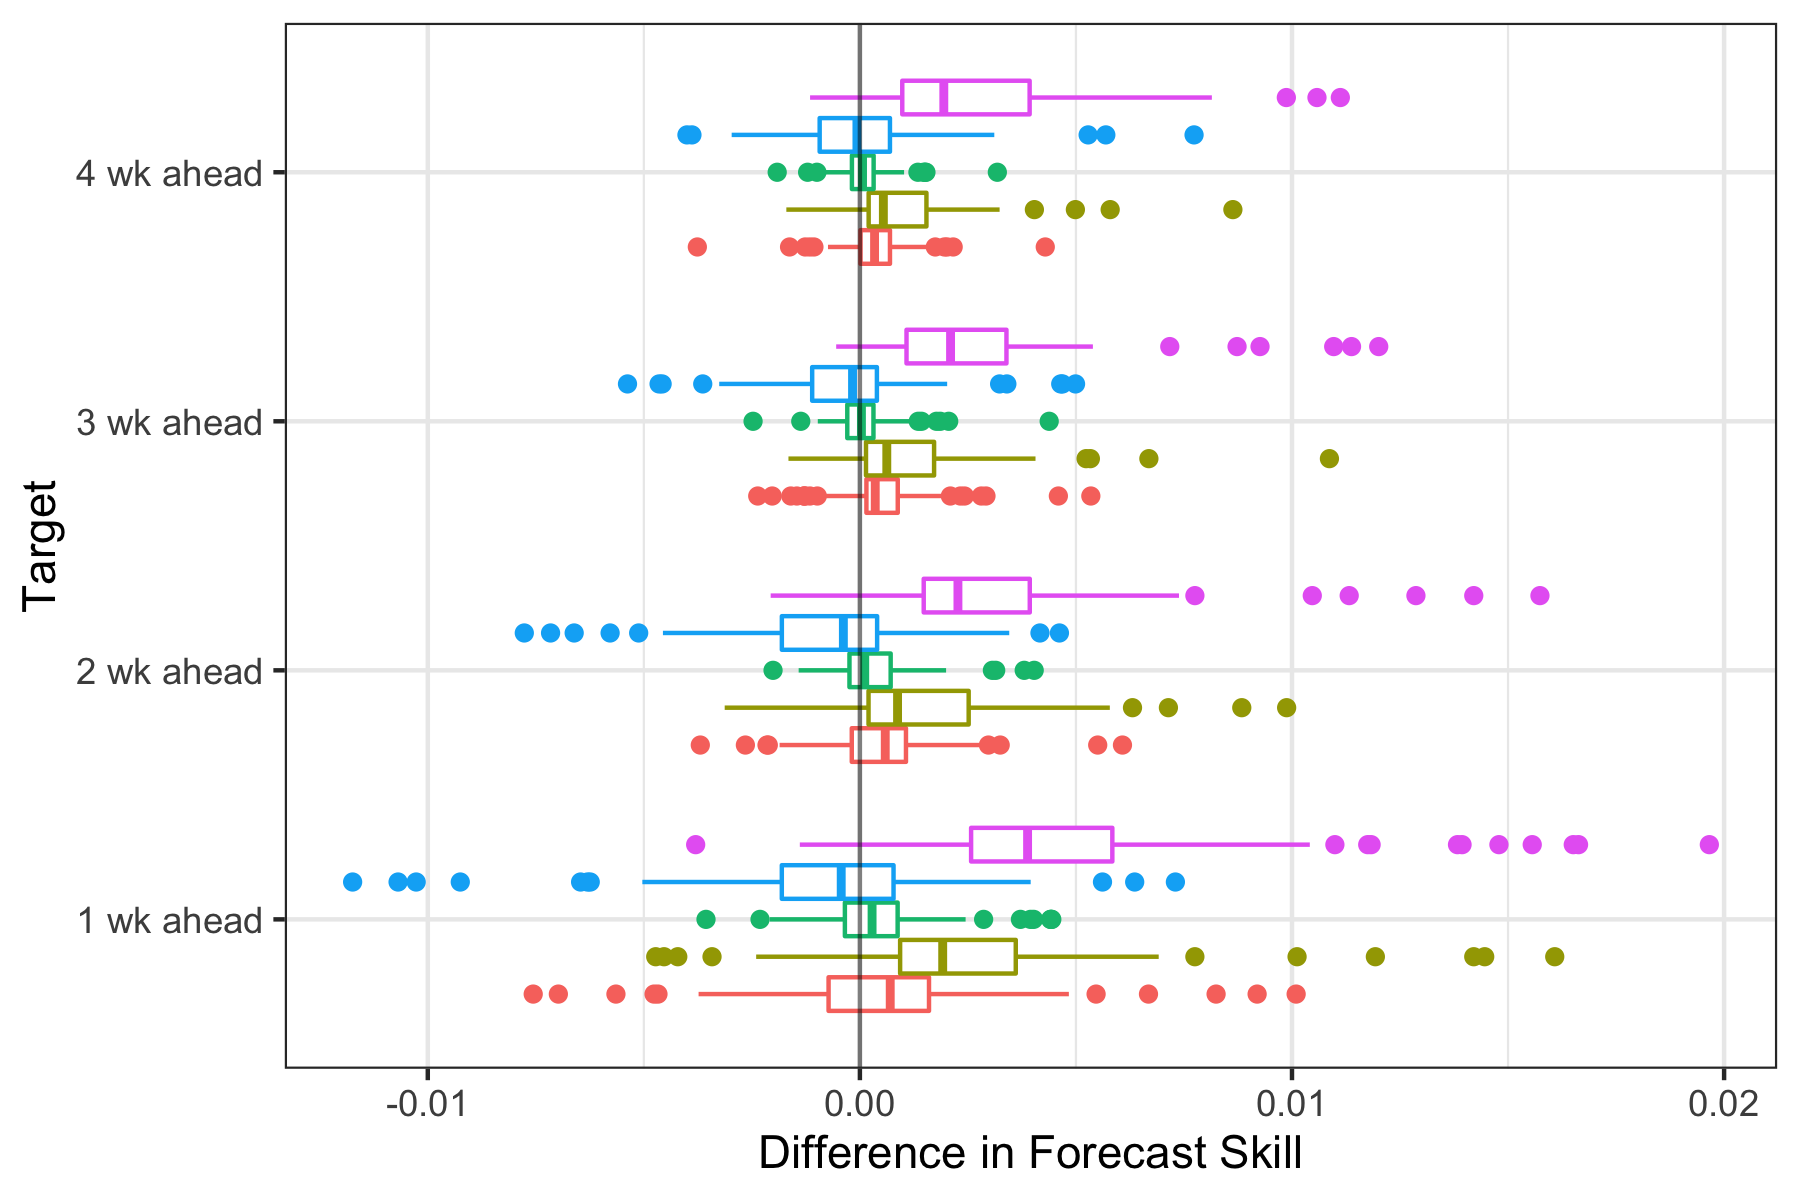
\includegraphics[scale=.14]{target.png}
\end{subfigure}
\begin{subfigure}{.5\textwidth}
  \centering
    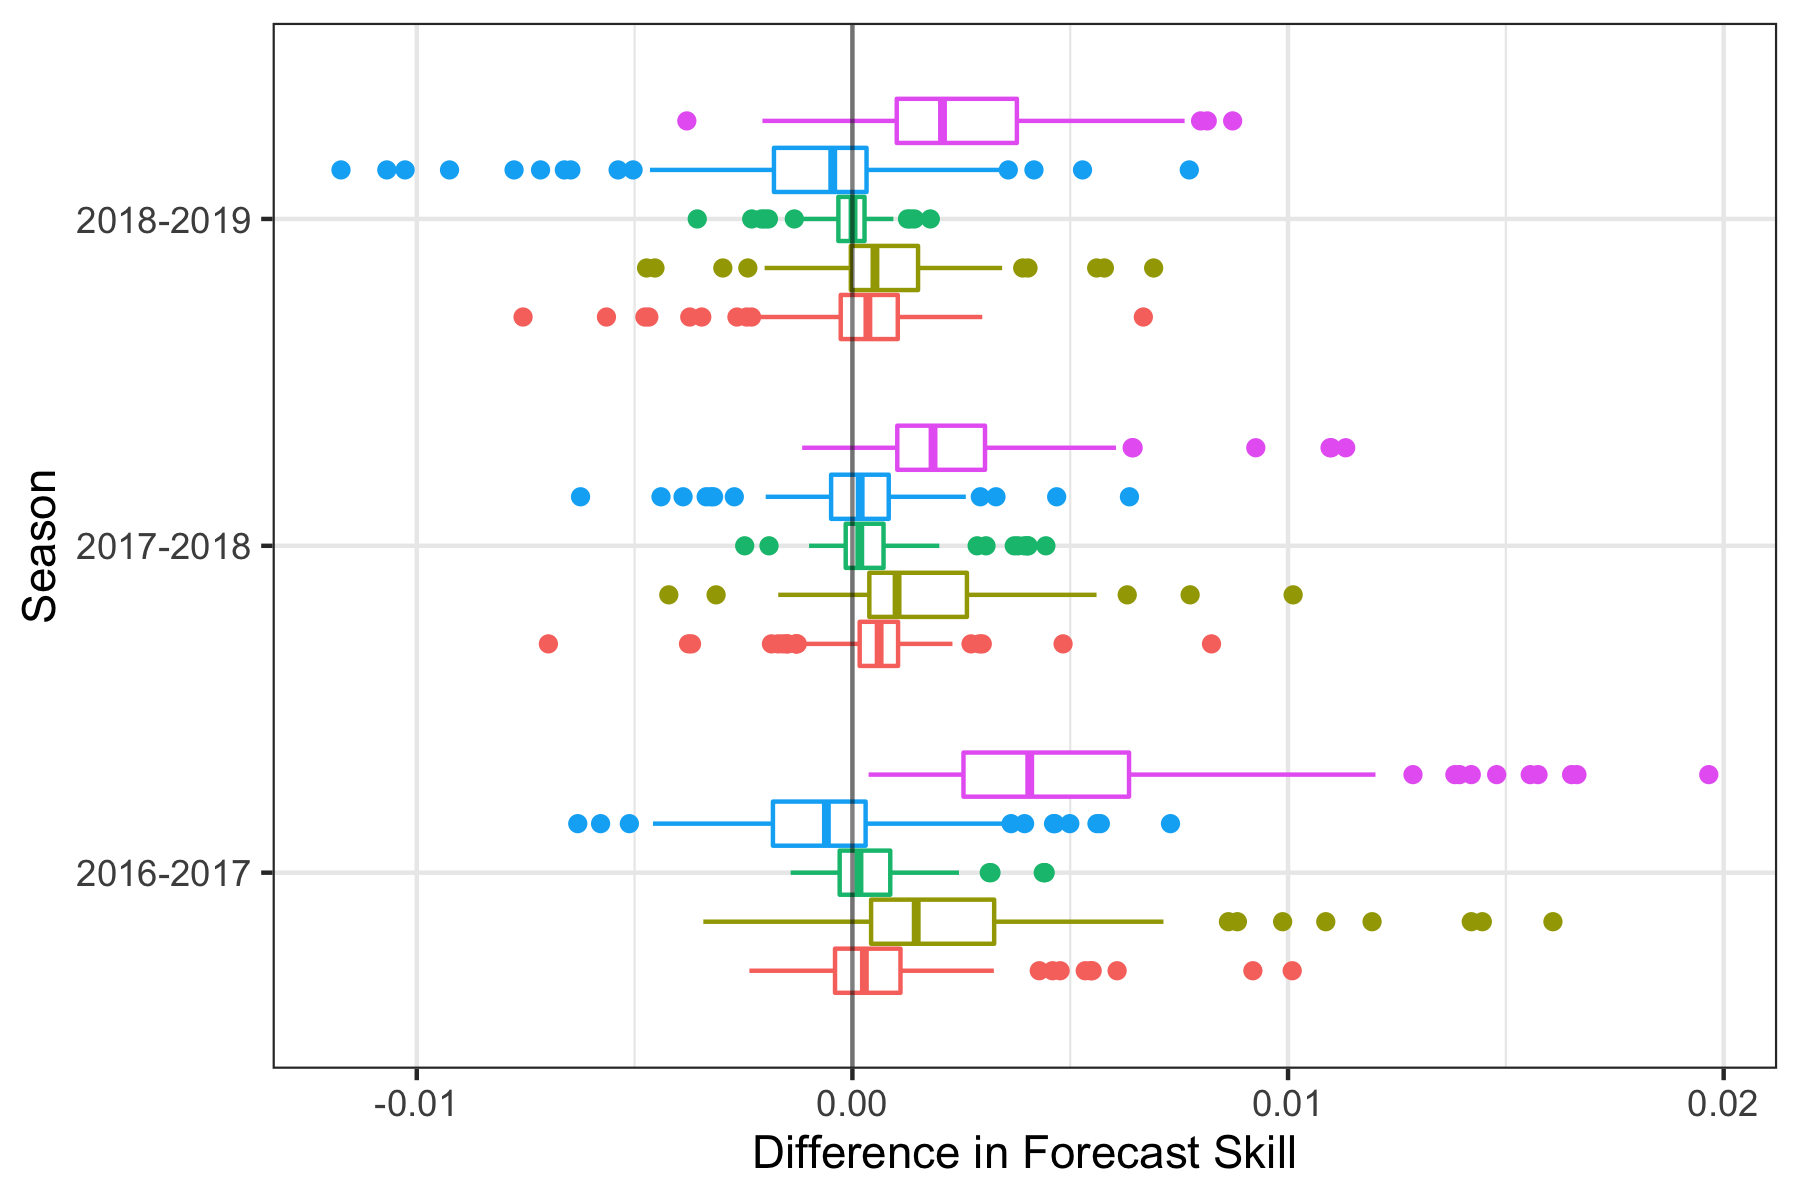
\includegraphics[scale=.14]{season_results.png}
\end{subfigure}
\begin{subfigure}{\textwidth}
  \centering
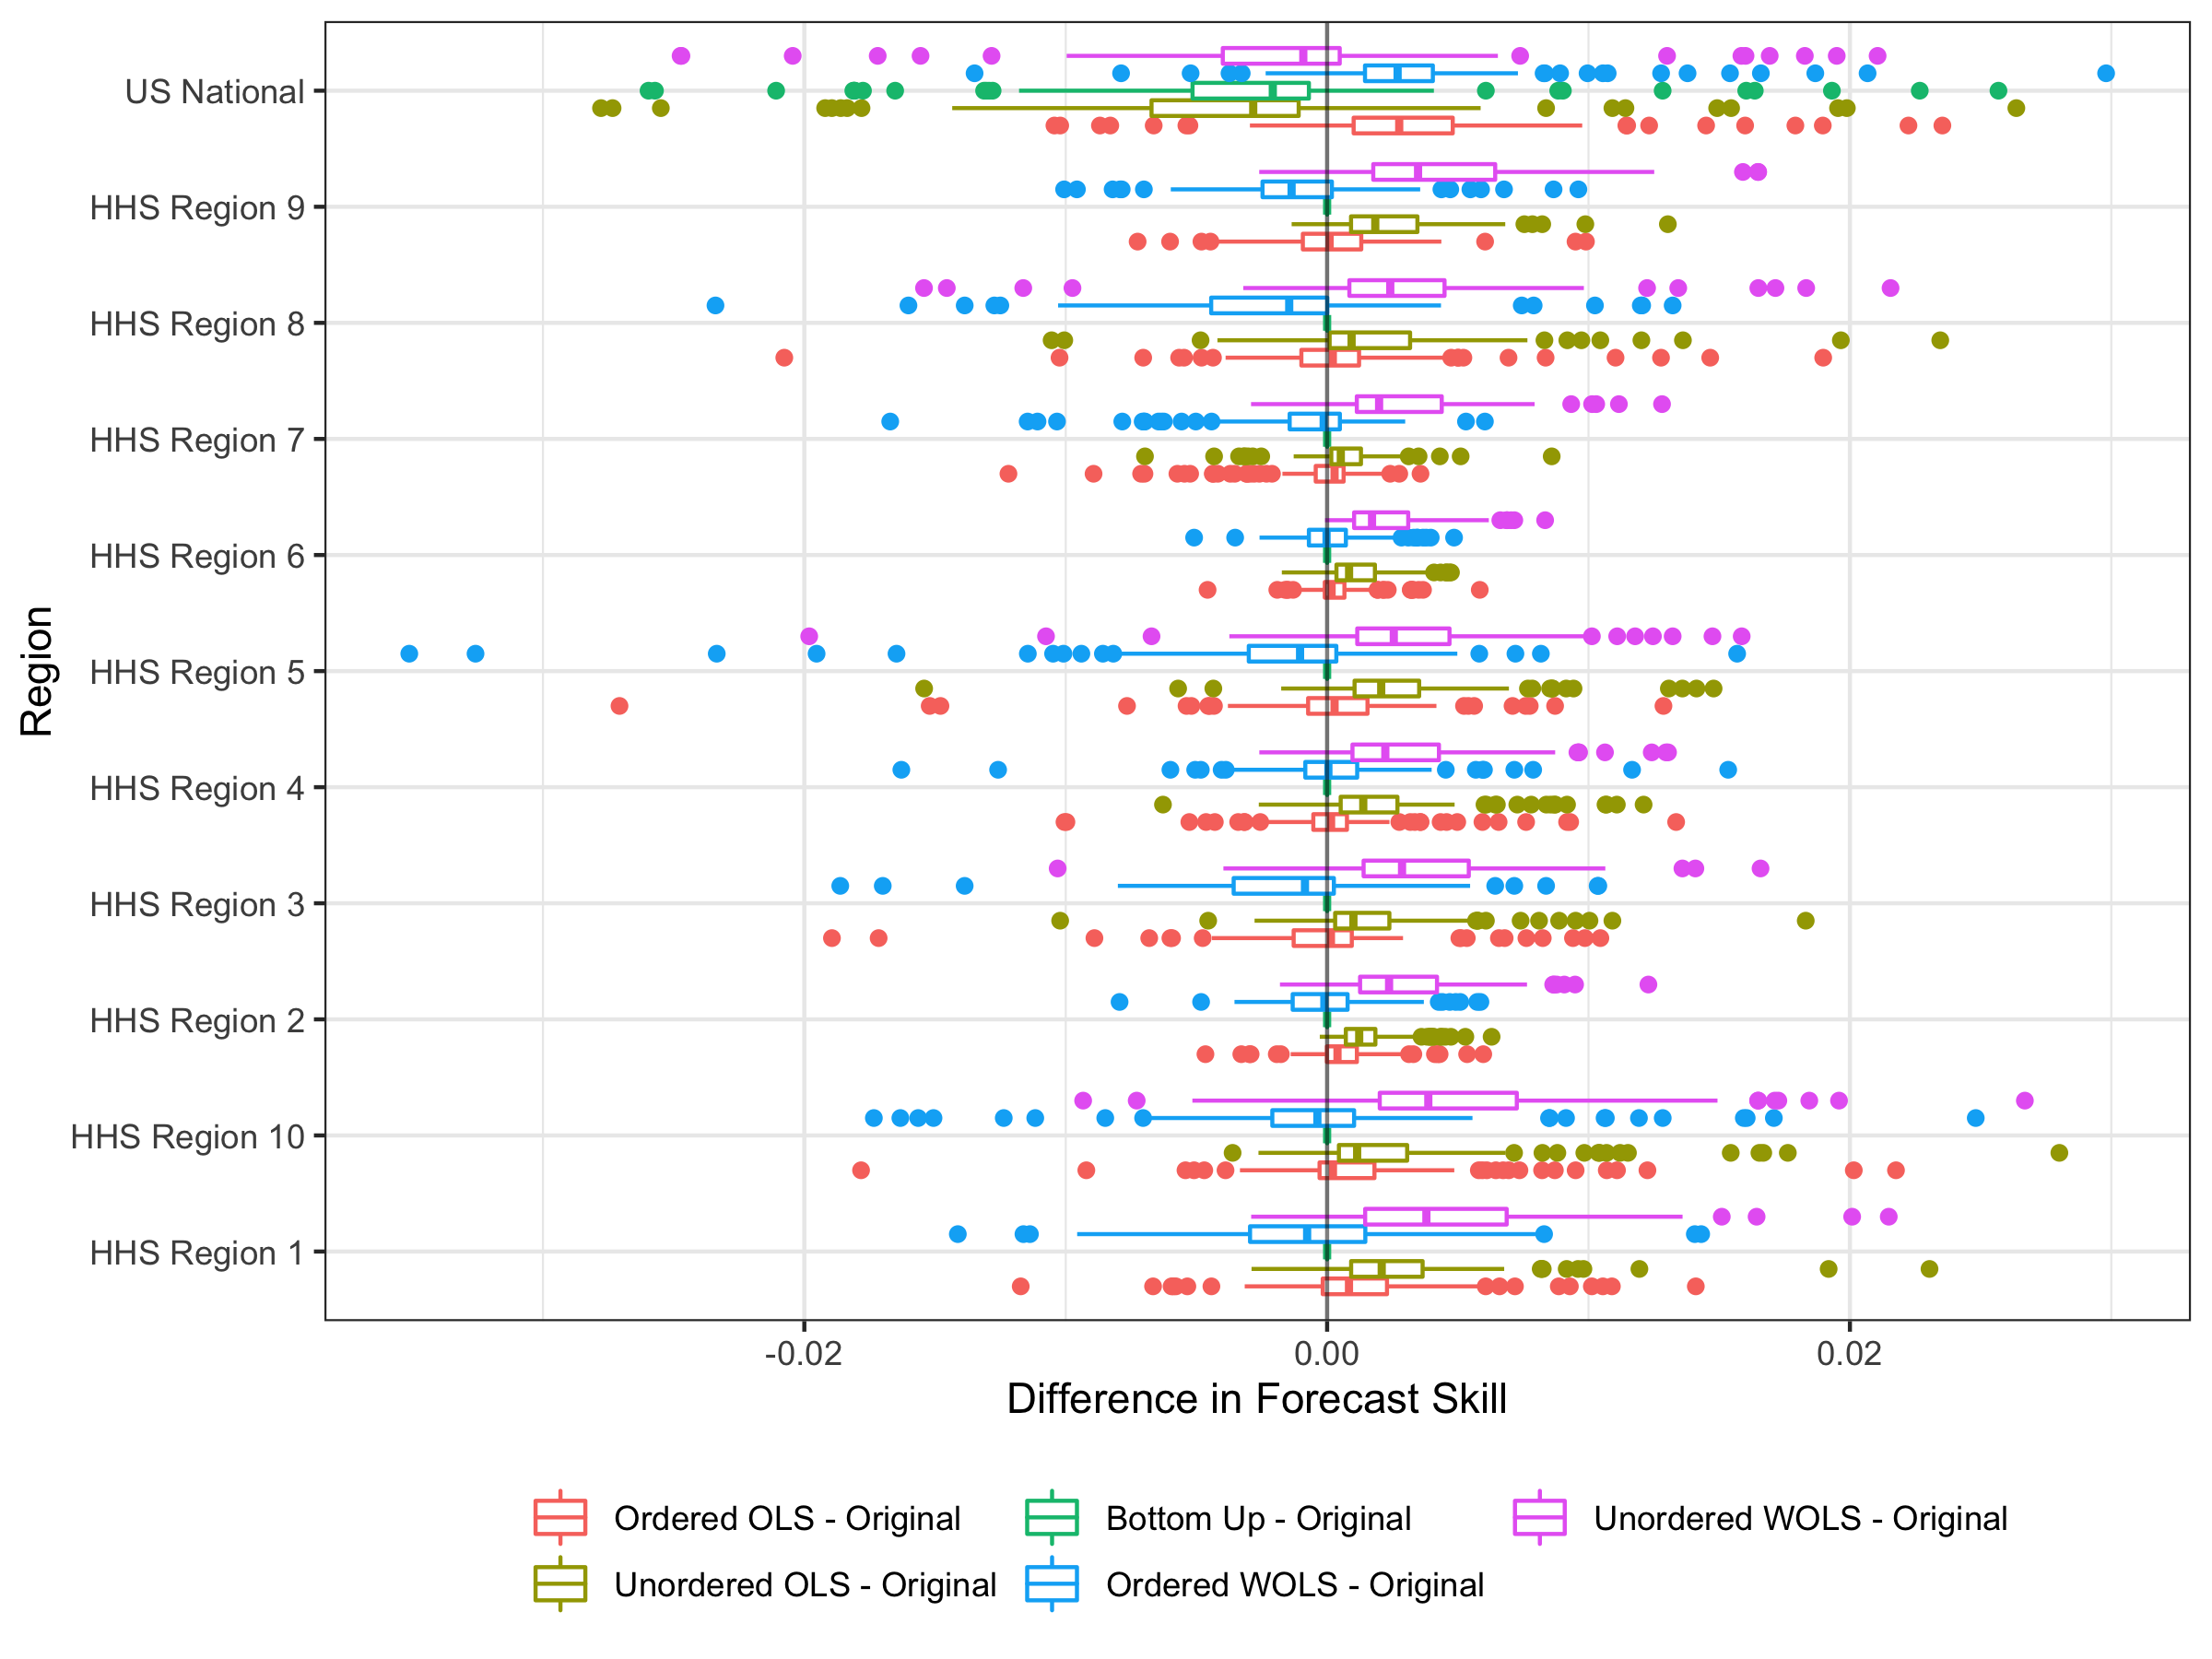
\includegraphics[scale=.175]{region_results.png}
\end{subfigure}

\caption{ Difference between single-bin forecast skill of projection method and forecast skill of independent forecasts averaged over all regions and epiweeks broken down by target (top-left), season (top-right), and region (bottom). Each point represents a single model-season combination. Box-whisker forecasts and  represent the inter-quartile range as well as the maximum and minimum in forecast skill difference between projected method and independent forecasts. The improvements in single-bin forecast skill are consistent across season and target for the unordered WOLS. However, the improvements are only consistent across the HHS regions, not the national region.}
\label{fig:region_results}
\end{figure}



The results are consistent across targets (see  Figure \ref{fig:region_results} top left), where a majority of model/season forecast skill improves over the forecast skill of the independent forecasts under the unordered WOLS method. The median increase in forecast skill under the unordered WOLS method was .0039 (variance 2.52e-05) at 1-week ahead, .0024 (variance 1.19e-05) at 2-week ahead, .0021 (variance 8.44e-06) at 3-week ahead and .0020 (variance 8.27e-06) at 4-week ahead. We can see that the difference in forecast skill diminishes as horizon increases. This suggests that coherence has the greatest benefit at shorter time horizons, where forecasts are more accurate. The other 3 projection methods do not show consistent improvement across targets.

We also break down the results by season (Figure \ref{fig:region_results} top right). Here we see that the unordered WOLS method consistently improves forecast skill, even under the 2017-2018 epidemic year. In the 2016-2017 season all but 4 models improved under the unordered WOLS method (Figure  \ref{fig:model_results} left), in 2017-2018 all but 4 models improved and in 2018-2019 all but 8 models improved. The magnitude of improvement does vary significantly by season. The median improvement in 2016-2017 was .0042 (variance 2.24e-05), in 2017-2018 was .0015 (variance 4.96e-06) and in 2018-2019 was .002 (variance 5.30e-06). The other three projection methods do not show consistent improvement across seasons.

Finally, the results are consistent across HHS regions (Figure \ref{fig:region_results} bottom) with the unordered WOLS method improving all HHS regions forecast skill. However, the forecast skill does not significantly change in the national region. The median improvement in HHS regions (excluding national) was 0.0028 (variance of 1.71e-05). The median decrease in the national level was -0.0008 (variance 5.59e-05).  We explore this result in the Discussion Section. The other three projection methods do not show consistent improvement across regions. 

 
\section{Discussion}
   
   Forecast coherence is a simple tool to improve forecast skill of short-term predictions in systems with hierarchical structures. In order to demonstrate this, we first defined probabilistic coherence, and showed that the results in the literature surrounding point forecast coherence do not naively transfer over to probabilistic forecasting. Guarantees for improvements in MSE do not directly transfer over to the CDC FluSight forecast skill metric of probabilistic forecast performance. However, by leveraging the definition of probabilistic coherence, we were able to generate coherent samples by first sampling from a collection of independent forecast distributions over all regions and projecting them onto a coherent subspace. This projection method is generic and allows for both correlated and uncorrelated projections and weighted and unweighted projections. By exploiting the underlying variability of the forecasts using normalized population size as a proxy for forecast variance, we were able to improve average forecast skill when broken down by model, season and target.
   
   In practice, the unordered and ordered OLS/WOLS methods are very appealing due to the lack of training data required and the operational simplicity of manipulating a submitted forecast, without requiring adjustments to the model code itself. No knowledge of the process model used to generate forecasts is required, only the resulting predictive density. Even though the benefits in forecast skill are small in magnitude, there is little cost to implementing coherence in practice and, especially for the unordered WOLS method, the frequency of forecasts improved is high (79\%).
   
   \begin{figure}
   \centering
    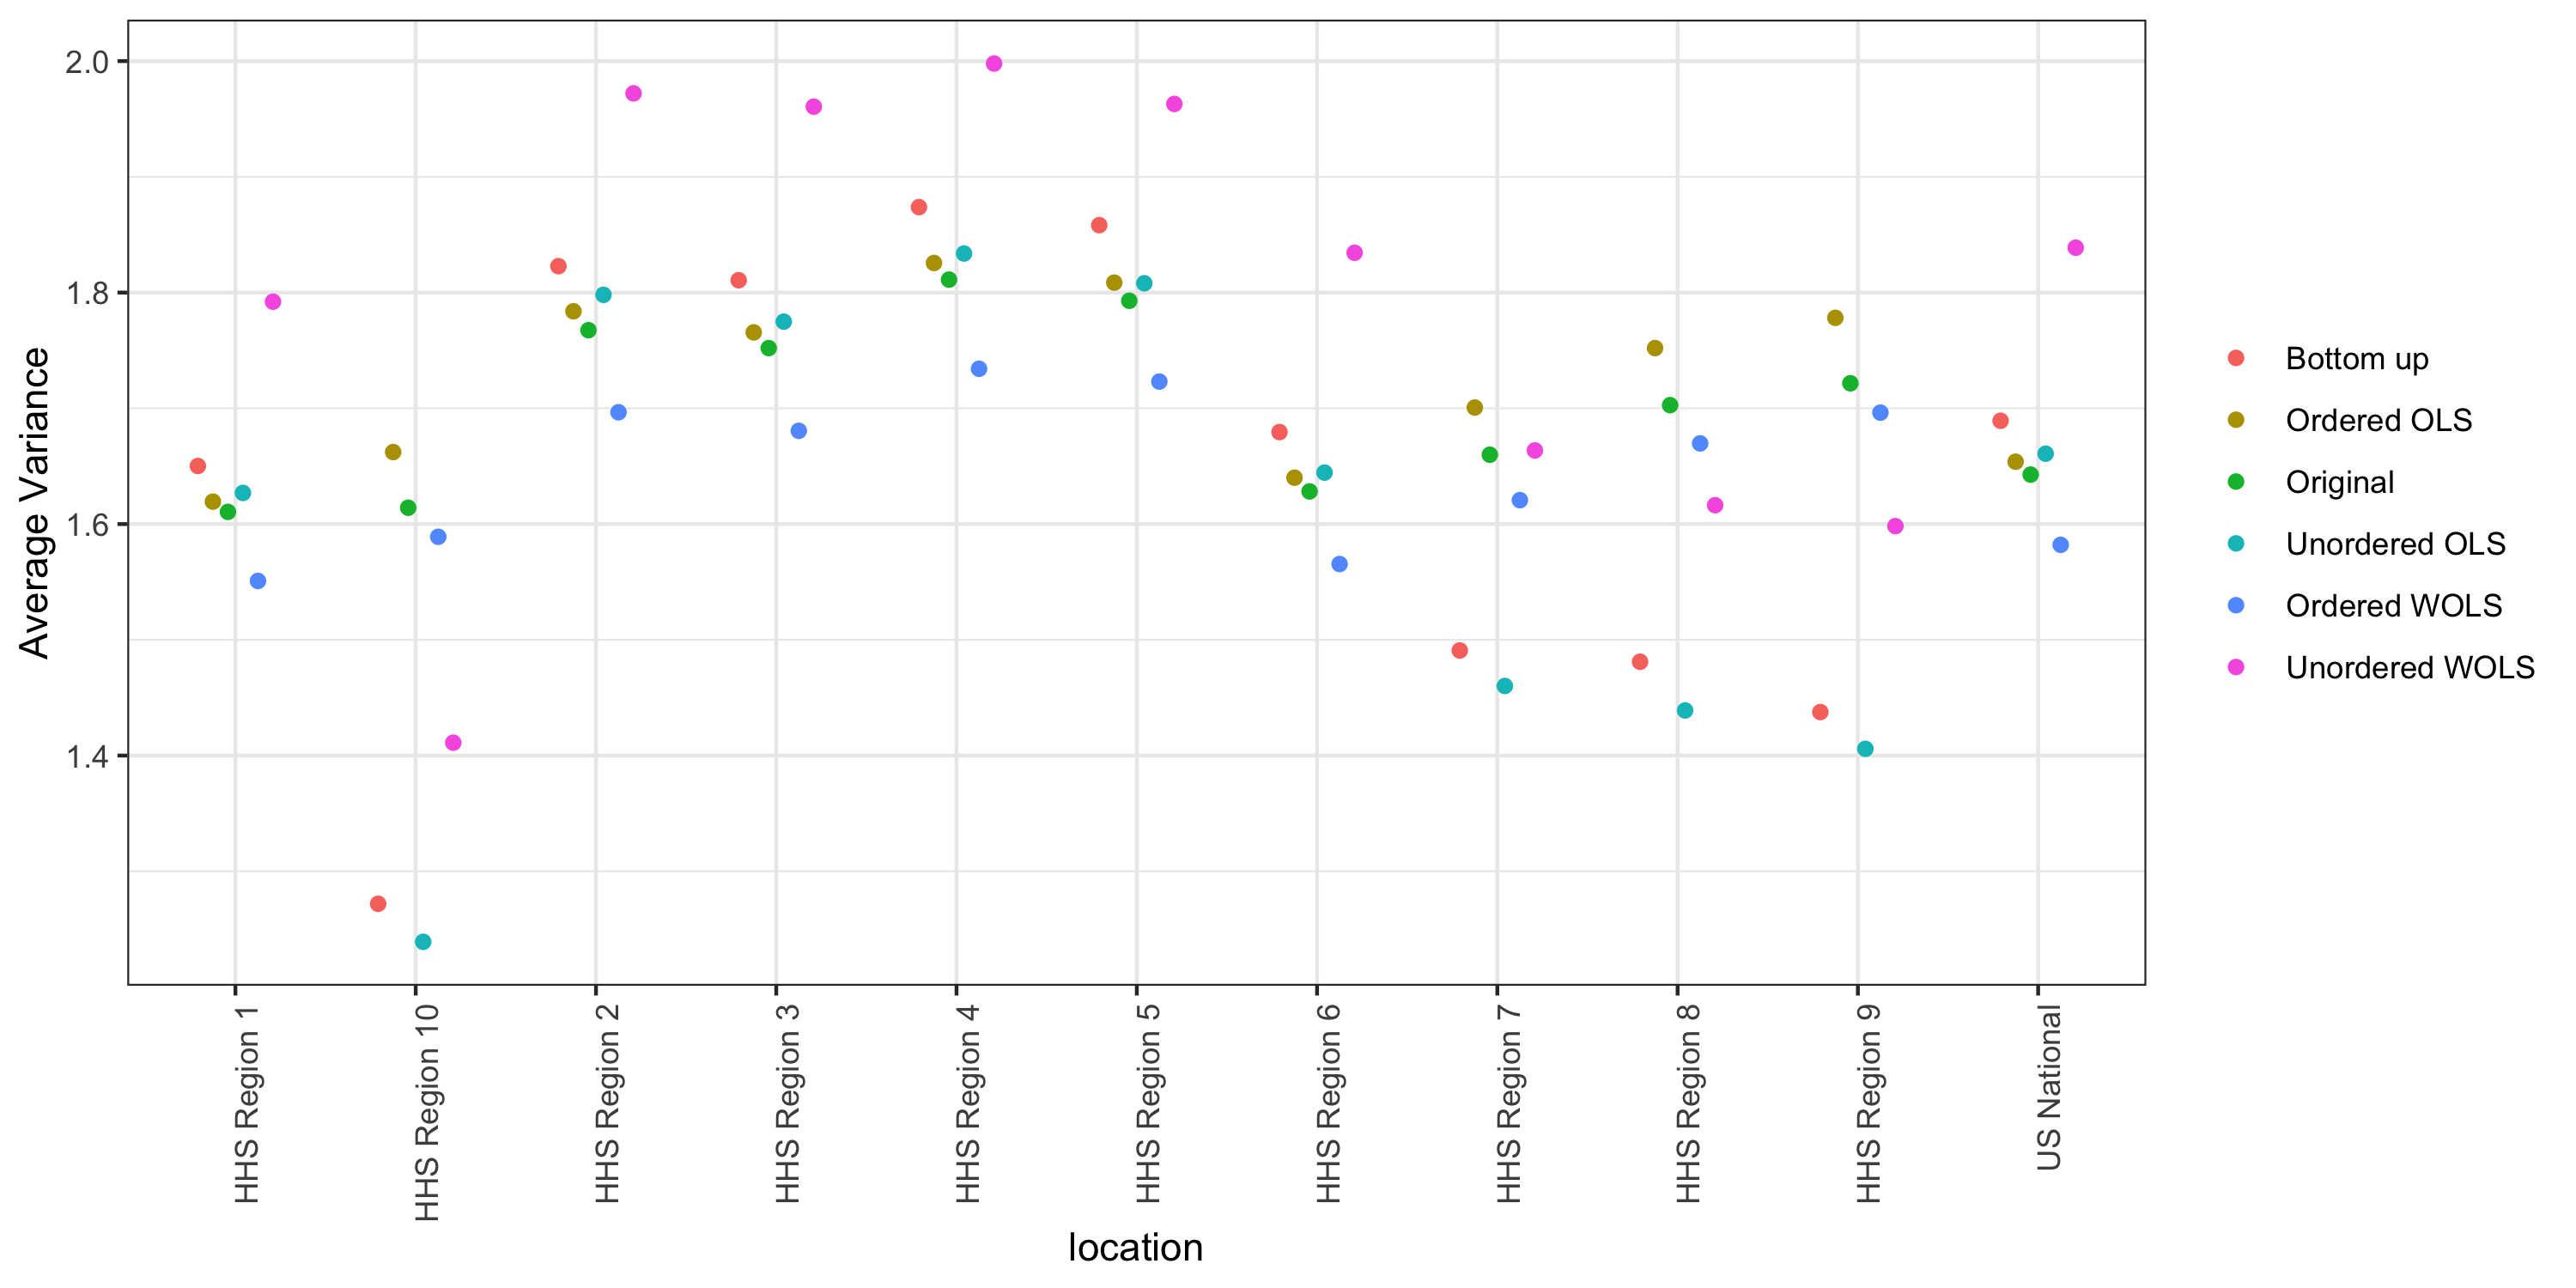
\includegraphics[scale=.15]{var.png}
    \caption{Average variance of forecasts, averaged over season, epiweek, target, and model. Notice that the unordered WOLS increases the variance across HHS regions, which is reflected in the improvements under single-bin scoring. However, the variance of the unordered WOLS decreases at the national level, which is also the only region without significant benefit under single-bin scoring. The optimal model under multi-bin scoring (ordered OLS) retains the same variance of the original forecast distribution for the HHS regions, but slightly increases the variance slightly for the nation. This demonstrates the effect of the scoring has on projection method choice.  }
    \label{fig:var}
\end{figure}

   
   Our experiments lead to the following conclusions:
     \begin{itemize}
   \item \textbf{Forecast coherence can benefit forecast skill, but the average benefits are small}. Using the unordered WOLS method, we can improve short-term forecast skill with high likelihood (79\% of model/seasons). We see a small improvement but with little to no cost in terms of parameter estimation and implementation difficulty. This makes the unordered WOLS method a clear choice to use when submitting forecasts to the CDC FluSight challenge. These benefits are consistent across region, season, and target breakdowns. While the improvements are modest, the .002 average increase in forecast skill is significant enough to change model rankings. In particular, in the 2018-2019 season, an average increase would have moved 3 out of 33 models up a ranking \cite{cdcscores}. However, some models do get worse under the unordered WOLS method, suggesting that forecasters implement coherence and perform interval cross-validation to decide.   
      
  \item \textbf{Weighting the forecasts by the variance of the region improves scores}. Under single-bin scoring, we see the biggest improvement when we take the variability of the forecasts by region into account. We do this by weighting the forecasts by the inverse of the population size of each region (where the nation receives weight 1). Region population size serves as a reasonable proxy for the underlying forecast variability, without relying on historical forecast data to estimate region variances. Regions with larger populations should in principal have more reliable forecasts. Using population size as an estimate of the variance, clearly demonstrates a benefit over the unordered OLS method which weights all forecast distributions equally. However, improvements may increase by weighting model specific region variances in the projection matrix. 

    
     
     \item \textbf{Coherence alters the variance of the forecasts} As we can see from Figure \ref{fig:var} the projection methods all change the average forecast variance when broken down by region. Under probabilistic scoring, this causes significant changes in the forecast skill of the methods. The optimal method under single-bin scoring is the unordered WOLS method. We can see from both Figure \ref{fig:var} and Figure \ref{fig:pcc_example} that the variance increases and the distribution is smoothed. This is a desirable property under single-bin scoring, where over-confident forecasts are penalized disproportionately (due to the asymmetry of the logarithm).  However, we also see that the variance of the unordered WOLS method is reduced in the National region. This corresponds with a lower average skill increase in the National region under the unordered WOLS method as seen in Figure \ref{fig:region_results}.
    
   \item \textbf{The naive bottom-up method does not perform as well as projection methods.} The bottom-up method is an intuitive coherence strategy with minimal implementation effort which ignores the independent national level forecast. Although it is appealing due to its simplicity, we were able to significantly improve forecast skill under both single-bin and mutli-bin scoring by using projection methods. 
   \item \textbf{Some models get worse under coherence methods.} For the 17 models that got worse under unordered WOLS method and single-bin scoring, the average variance of the forecast distribution across all models, targets, locations, and seasons was 2.36, whereas the average variance of the forecast distribution across all models, targets, locations, and seasons was 1.77. This suggests that models that already are highly variable may not improve. However, we would require more detailed model information to completely ascertain why some models decreased in skill and others improved. 
   \item \textbf{The choice of scoring rule matters}. We can see that the optimal method for single-bin scoring is not the optimal method for multi-bin scoring. The optimal projection method for single-bin scoring is unordered WOLS, which only showed $53\%$ of forecasts improving under multi-bin, the lowest of any other methods. The optimal projection method under multi-bin scoring is ordered OLS, which only showed a $51\%$, the third lowest of any other method. This suggests that single-bin and multi-bin scoring are capturing different features of the forecast distribution. As seen in Figure \ref{fig:var}, the unordered WOLS method increased the variance of the forecast distribution relative to the original forecasts. However, the ordered OLS method only slightly increased the variance of the forecast distribution relative to the original forecasts. This suggests that widening the variance under single-bin scoring increases forecast skill on average, which is consistent with single-bin scoring only counting probability density that falls exactly over the bin containing the truth. However, recent research has shown that multi-bin scoring is an approximation to common proper scoring rules such as the continuous rank probability score \cite{scoring}. This suggests that in the broader probabilistic forecasting realm, the results under the multi-bin scoring rule might be more applicable.    
   
   \end{itemize}
   
   
  
   
   
   Although projection methods are simple to implement and result in small but significant changes in forecast skill, there is still significant room for improvement. Recent work by Taieb et. al has explored copula based techniques to combine the independent forecast distributions from the regional level into a joint distribution with a specified covariance structure \cite{taieb2017coherent}. Wickramasuriya et. al have also explored various projections using a weighted least squares method \cite{wickramasuriya2015forecasting}. This weight matrix also represents the correlation structure between the independent forecasts but can be estimated from historical forecast accuracy. It is clear that, unlike in the point forecast setting, exploring various correlation structures in the probabilistic setting has a drastic effect on the results. Given historical training data, one could estimate the error correlation specific to a given process model which could potentially lead to an even greater increase in forecast skill. However, in the absence of historical training data, forecasters can still leverage coherence to improve probabilistic forecast skill. In all, these results suggest that simple and fast methods can improve probabilistic forecasts of systems where the available data has a natural hierarchy. In practice, we recommend using cross-validation to choose the appropriate method for an individual forecasting model. While the results suggest that unordered WOLS is the correct choice, Figure \ref{fig:model_results} shows that some models may decrease in skill, so internal validation is advised.  Using the example of seasonal influenza forecasts in the US, we show that enforcing coherence provides a high likelihood of improvement in forecast accuracy, and in general may provide opportunities for improvement in forecast accuracy in this and other real-world application settings.
 

   
   
   
   
  \newpage
 
\section{Appendix A}

\begin{theorem}
Let $\boldsymbol{X}_{n \times p}$ be a matrix of full column rank. Assume $\bm{y} \in$ colspace($\boldsymbol{X}$), $\tilde{\bm{y}} = \bm{y}+ \bm{\delta}$ where $\bm{\delta} \in \mathbb{R}^n$, and
$\hat{\bm{y}} = \boldsymbol{P} \tilde{\bm{y}}$, where $\boldsymbol{P} = \boldsymbol{X}(\boldsymbol{X}^T\boldsymbol{X})^{-1}\boldsymbol{X}^T$.
Then, $||\tilde{\bm{y}} - \bm{y}||_2 \geq ||\hat{\bm{y}} - \bm{y}||_2$.

\end{theorem}


\begin{proof}
Properties for the proof:
\begin{enumerate}
\item[Property 1:] Let $\boldsymbol{X}$ be an $n \times p$ matrix such that rank($\boldsymbol{X}$) $= p$.
\item[Property 2:] Define $\boldsymbol{P} = \boldsymbol{X}(\boldsymbol{X}^T\boldsymbol{X})^{-1}\boldsymbol{X}^T$. Then
\begin{enumerate}
\item[Property 2a:] $\boldsymbol{P}$ is idempotent (i.e., $\boldsymbol{P} = \boldsymbol{P} \boldsymbol{P} = \boldsymbol{P}^2$).
\item[Property 2b:] $\boldsymbol{P}$ is symmetric (i.e., $\boldsymbol{P} = \boldsymbol{P}^T$).
\item[Property 2c:] $\boldsymbol{I-P}$ is idempotent.
\item[Property 2d:] $\boldsymbol{I-P}$ is symmetric.
\end{enumerate}
\item[Property 3:] If $\boldsymbol{A}$ is a symmetric matrix, then $\boldsymbol{A} = \boldsymbol{Q} \boldsymbol{\Lambda} \boldsymbol{Q}^T$ where $\boldsymbol{Q}$ is a matrix whose columns are equal to the eigenvectors of $\boldsymbol{A}$ and $\boldsymbol{\Lambda}$ is a diagonal matrix whose diagonal elements $\lambda$ are the eigenvalues of $\boldsymbol{A}$.
\item[Property 4:] If $\boldsymbol{A}$ is idempotent, then its eigenvalues are either 0 or 1.
\item[Property 5:] Assume $\bm{y} \in $ colspace($\boldsymbol{X}$).
\item[Property 6:] $\tilde{\bm{y}} = \bm{y} + \bm{\delta}$, where $\bm{\delta} \in \mathbb{R}^n$.
\item[Property 7:] $\hat{\bm{y}} = \boldsymbol{P}\tilde{\bm{y}}$
\end{enumerate}

The proof proceeds as follows:
\begin{align*}
||\tilde{\bm{y}} - \bm{y}||_2 - ||\hat{\bm{y}} - \bm{y}||_2 &= ||\bm{y} + \bm{\delta} - \bm{y}||_2 - ||\boldsymbol{P}\tilde{\bm{y}} - \bm{y}||_2 \tag*{(Properties 6 and 7)}\\
&= ||\bm{\delta}||_2 - ||\boldsymbol{P}\bm{y} + \boldsymbol{P}\bm{\delta} - \bm{y}||_2 \tag*{(Property 6)} \\
&= ||\bm{\delta}||_2 - ||\bm{y}  + \boldsymbol{P}\bm{\delta} - \bm{y}||_2 \tag*{(Property 5)}\\
&= ||\bm{\delta}||_2 - ||\boldsymbol{P}\bm{\delta}||_2 \\
&= \bm{\delta}^T\bm{\delta} - \bm{\delta}^T\boldsymbol{P}^T \boldsymbol{P} \bm{\delta} \\
&= \bm{\delta}^T\bm{\delta} - \bm{\delta}^T\boldsymbol{P} \boldsymbol{P} \bm{\delta} \tag*{(Property 2b)}\\
&= \bm{\delta}^T\bm{\delta} - \bm{\delta}^T\boldsymbol{P} \bm{\delta} \tag*{(Property 2a)}\\
&= \bm{\delta}^T ( \boldsymbol{I} - \boldsymbol{P}) \bm{\delta} \\
&= \bm{\delta}^T \boldsymbol{Q} \boldsymbol{\Lambda} \boldsymbol{Q}^T \bm{\delta} \tag*{(Properties 2d and 3)}\\
&= \bm{a}^T \boldsymbol{\Lambda} \bm{a} \tag*{(where $\bm{a} = \boldsymbol{Q}^T \bm{\delta}$)}\\
&= \sum_{i=1}^n \lambda_i a_i^2 \tag*{(Property 3)}\\
&\geq 0. \tag*{(Properties 4 and 2c)}
\end{align*}
\noindent Thus, $||\tilde{\bm{y}} - \bm{y}||_2 - ||\hat{\bm{y}} - \bm{y}||_2 \geq 0$ implies $||\tilde{\bm{y}} - \bm{y}||_2 \geq ||\hat{\bm{y}} - \bm{y}||_2$.
\end{proof}

\chapter{Accounting for delay}

 Since 2013, the CDC has organized an influenza forecasting challenge that brings together modellers and public health officials from across the U.S. in an effort to generate probabilistic forecasts of influenza-like-illness (ILI). The CDC defines ILI as a ratio of patients presenting with a cough and fever over 100 over the total number of patients. They release weekly ILI data across 10 health and human services regions (HHS) as well as a nationally. However, the initial estimate of ILI may be revised as more providers in a given HHS region report both the number of patients that tested positive for ILI symptoms and the total number of patients. Many models in the competition take the ILI reporting revisions into account when forecasting. However, the effects of controlling for these revisions across various process models has yet to fully understood. We present a detailed exploratory analysis of the sources of reporting revisions, the effects on the available ILI, and the consequences on forecast skill. 


\section{Importance of Influenza Forecasting}


Seasonal influenza hospitalizes over half a million people in the world every year\cite{lafond2016global}.
The United States alone reported approximately 80,000 Influenza related mortalities in the 2017/2018 influenza season, with most serious consequences for vulnerable populations such as children or the elderly. The annual toll of influenza outbreaks in the US provide a frequent reminder of the importance of interventions that could help mitigate the impact of influenza outbreaks.\cite{skowronski2018early}


The main tool in the fight against influenza is vaccination. The CDC recommends that everyone, including children, get vaccinated at the beginning of the season. However, there are only a finite number of vaccines produced each season, begging the question of how to best allocate the limited number of vaccines to protect the largest number of at risk people. Studies have shown that an optimal allocation of influenza vaccine requires an accurate estimate of risk to the population. \cite{mylius2008optimal} To this end, accurate probabilistic forecasting models may help with optimal risk assessment and therefore optimal allocation. 


As part of their forecasting initiative, the CDC releases forecasts for weighted influenza-like illness (wILI), which measures the proportion of outpatient doctor visits at reporting health care facilities where the patient had influenza-like illness, weighted by state population. Forecasts are made for up to four weeks into the future, as well as seasonal targets including week of peak incidence, peak week wILI value and season onset. Participants in the FluSight challenge have harnessed a variety of models and methods to forecast the targets under consideration. These efforts have included time series models, mechanistic transmission models, and machine learning techniques.\cite{kandula2018evaluation} Five teams submitted forecasts from seven models in the 2017/2018 season.\cite{biggerstaff2018results} Some teams have also incorporated external data to improve forecasts.\cite{dugas2013Influenza}\cite{araz2014using}\cite{volkova2017forecasting}


However, many submitted models fall prey to reporting revisions. Each week, the CDC releases updated data that include an initial report of wILI for a particular week as well as revisions to previously reported wILI. These revisions occur for a variety of reasons, and initial reports of wILI may be revised upwards or downwards. For example, initial reports of wILI may be revised upwards if additional cases of ILI are reported or revised downwards if additional outpatient doctor visits without ILI are reported. These revisions have consequences for forecast accuracy since the way the CDC assesses model performance by evaluating forecasts generated using unrevised data are able to predict the revised final data at the end of the season.\cite{reich2019collaborative} Revisions may occur up to 10 weeks after the final week of the season, after which the CDC fixes the observed data at that time as the "truth", for purposes of scoring models. Accounting for revisions in real-time may improve log-score on CDC defined targets by recognizing patterns in historical revisions and applying them to currently reported data. 

Methods for accounting for reporting revisions have commonly been referred to as "nowcasting" in the literature. This is because we are providing an estimate of a desired signal at the current time (commonly called time "now") based on a partially observed signal.\cite{lawless1994adjustments} \cite{lampos}\cite{johansson2014nowcasting} Early attempts at correcting for reporting revisions focused solely on the under-reporting aspect. \cite{kalbfleisch1989inference} The work of Lawless et al. used a non-parametric method to scale up observed incidence levels of human immunodeficiency virus (HIV) based on historical revisions in order to gain a more accurate estimate of the emerging HIV epidemic. Hohle extended this effort to account for arbitrary transmission models in an under-reported setting during a Shiga toxin-producing E. coli epidemic. \cite{hohle2014bayesian} Recently, Nunes et al. employed a hidden Markov model to estimate the reporting revisions to wILI data from Portugal with success. \cite{nunes2013nowcasting} Stone et al. also investigated the application of state space models to the reporting delay problem with count data in a hierarchical setting.\cite{stoner2019multivariate}

With respect to influenza-like-illness in the U.S., much of the current efforts are focused on using external data to improve the estimates of the unrevised data. External data show significant improvements to 1-4 week ahead forecasts but not to seasonal forecasts.\cite{osthus2019even} Reporting delay has previously been modeled without using external data at the national level with mixed results for the 1-4 step ahead targets. \cite{brooks2018nonmechanistic} We propose a framework that lends itself to modeling delay at both the national and state level and suggest models that improve both seasonal and short term forecast log scores at both the national and state level.


\section{US ILI Surveillance Data}

For the national challenge, the CDC wILI data are provided at both the national level and broken down into 10 Health and Human Services (HHS) regions, mostly organized by geographical proximity. The national level data extend from 1997 to the present and the HHS regional data are available starting from 2013. The revised wILI data are highly seasonal and vary by region (Figure \ref{fig:data-overview}A). For the state level challenge, only data from 2016 to the present is available. Data is reported for each state at the ILI level, except for Florida, which does not participate. 

These data are reported by the ILINet system, a consortium of over 3,500 outpatient healthcare facilities across all states and territories in the US. Each week, around 2,200 of these providers report both total number of patient visits and total number of patients presenting with influenza-like symptoms. These two numbers are combined to report the percentage of cases reporting with influenza-like symptoms and are weighted by population size of the state to generate the final regional or national wILI level. \cite{cdc_flusight}

The CDC releases updated wILI data on a weekly basis for all states and regions. These updates include new wILI estimates for the most recent week, in addition to revisions for all prior weeks of the season. As noted above, revisions can be made either upwards or downwards due to updates to both the total number of visits and total of number of ILI visits. An example of historical revisions is shown in Figure \ref{fig:data-overview}B). Revision data extends back to 1997 for the national level data, but only includes the 2017/2018 season for state level data. 


In the following analysis we consider only the initially reported and finally revised wILI values for a given epiweek $w$. This is because when forecasting from epiweek $w$ in real-time we only have access to the initially reported wILI value for epiweek $w$. Modifications to the forecast for epiweek $w+h$ should therefore be based on potential revisions to the initially reported data. Differences between initially reported and finally revised ILI is shown in Figure \ref{fig:diff_v_final_ili}






\subsection{Targets}

The CDC FluSight challenge identifies three key seasonal targets of interest: season onset, season peak week percentage, and season peak week. Season onset is defined as the first week of the season which exceeds a pre-specified baseline for at least 3 consecutive weeks. That is, the week at which we have observed three wILI  values above a set baseline in a row. This is helpful for public health officials in their preparation and planning for the upcoming season. This target is restricted to national and regional level data, where such baselines are defined. This definition makes season onset particularly susceptible to reporting revisions. Revising the wILI just slightly can flip the wILI value above or below the pre-specified season onset, and therefore change the identified season onset week. Season peak week percentage is defined as the maximum wILI or ILI value observed for the season. This target is also sensitive to reporting revisions if a season peak percentage value that has been observed is revised downwards. This is because forecasting models can only place probability of a season peak percentage larger than the observed peak percentage. Finally, season peak week is defined as the week in which the maximum observed wILI value occurs. This target is less sensitive to reporting revisions since revisions usually respect the relative ordering of wILI or ILI values within a season. This is also in part because of the relatively consistent direction of reporting revisions throughout a season.  
  In addition to seasonal targets the CDC is interested in 1-4 week ahead forecasts for short term projections of ILI. These are helpful for real-time public health decision making and resource allocation. In practice, the data is delivered with a two week lag, so the 1 step head forecast is actually a "hindcast", the 2 step ahead forecast is a "nowcast", and the 3-4 step ahead forecast is a true forecast. 


\subsection{Scoring}

In order to score the probabilistic forecasts the CDC uses a "single-bin" log score in the FluSight challenge. If we index each of the predictive distributions for target $Z_t$ at week $w$ for bin $i$ by region $r$ and season $s$   we obtain a discrete distribution of the form,

$$p_{r,s,w,Z_t,i} = P_{r,s,w}(Z_{t} =i)$$

For example, if $Z_t = \text{1 Wk Ahead}$ then $i = \{0,.1,.2,....,13,13+\}$ and if $Z_t = \text{Season Onset}$ then $i=\{1,...,52\}$. We therefore have that $\sum_i p_{r,s,w,Z_t,i} = 1$. We compute the log score of a forecast as the log of the probability assigned to the observed outcome In order to avoid $-\infty$ when the probability assigned to the target is $0$ we truncate at -10, following convention set by the CDC. 

\begin{equation}
\text{log score}_{r,s,w,Z_t} = max(-10,log( p_{r,s,w,Z_t,i}))
\end{equation}



\subsection{Revisions}
\subsubsection{Sources of Revision}

There are two main sources of revisions. 

\begin{itemize}
    \item Providers not reporting both their number of patients positive for ILI and total number of patients in the epiweek they occurred
    \item Providers revising an estimate they previously reported 
\end{itemize}

We handle each case separately because of the different ramifications each revision process has on the reported ILI value. 

If providers simply do not send their data into the CDC by the deadline for a given epiweek, this is reflected in the \textbf{number of providers} the CDC estimate is based on. Unfortunately, this information alone is not enough to accurately adjust the ILI towards the final reported ILI. This is because of proportion definition of ILI. 

\begin{equation}
    ILI_{new} = \frac{\text{num ILI}_{old} + \text{num ILI}_{new}} {\text{num patients}_{old} + \text{num patients}_{new}}
\end{equation}


As we can see from equation 3, $ILI_{new}$ can be either greater or less than $ILI_{old}$ depending on the relative contribution of $\text{num ILI}_{new}$ to the numerator and $\text{num patients}_{new}$ to the denominator. Thus, just because providers have not reported their data, does not mean ILI will go up. This makes the problem of predicting backfill quite difficult. Existing methods have used the number of providers as an indicator of uncertainty around the available ILI, but not as an indicator of the direction the ILI will be revised. This is shown in \ref{fig:revisions_by_prov} where we examine the difference between the number of providers initially reported versus the number of providers reported at the end of the season for a given epiweek. As expected, as the difference in the initial providers and final providers gets smaller, the difference in the initial number of ILI positive patients versus the final number of ILI positive patients also decreases. Similarly, the difference in the total number of patients initially reported versus the number of paitents finally reported also decreases (tends towards 0). However, because ILI is a proportion of the two, as the difference in the initial number of providers and final number of providers goes to 0, the difference in initial ILI and final ILI displays no clear trend. 




The other way in which available ILI may be revised is through revisions to data already reported by providers. These revisions are again unpredictable in direction, but are also unpredictable when they occur. Unfortunately, the have significant effect on reported wILI (ILI) as shown in \ref{fig:same_prov_diff} 


\begin{figure}[H]
    \centering
    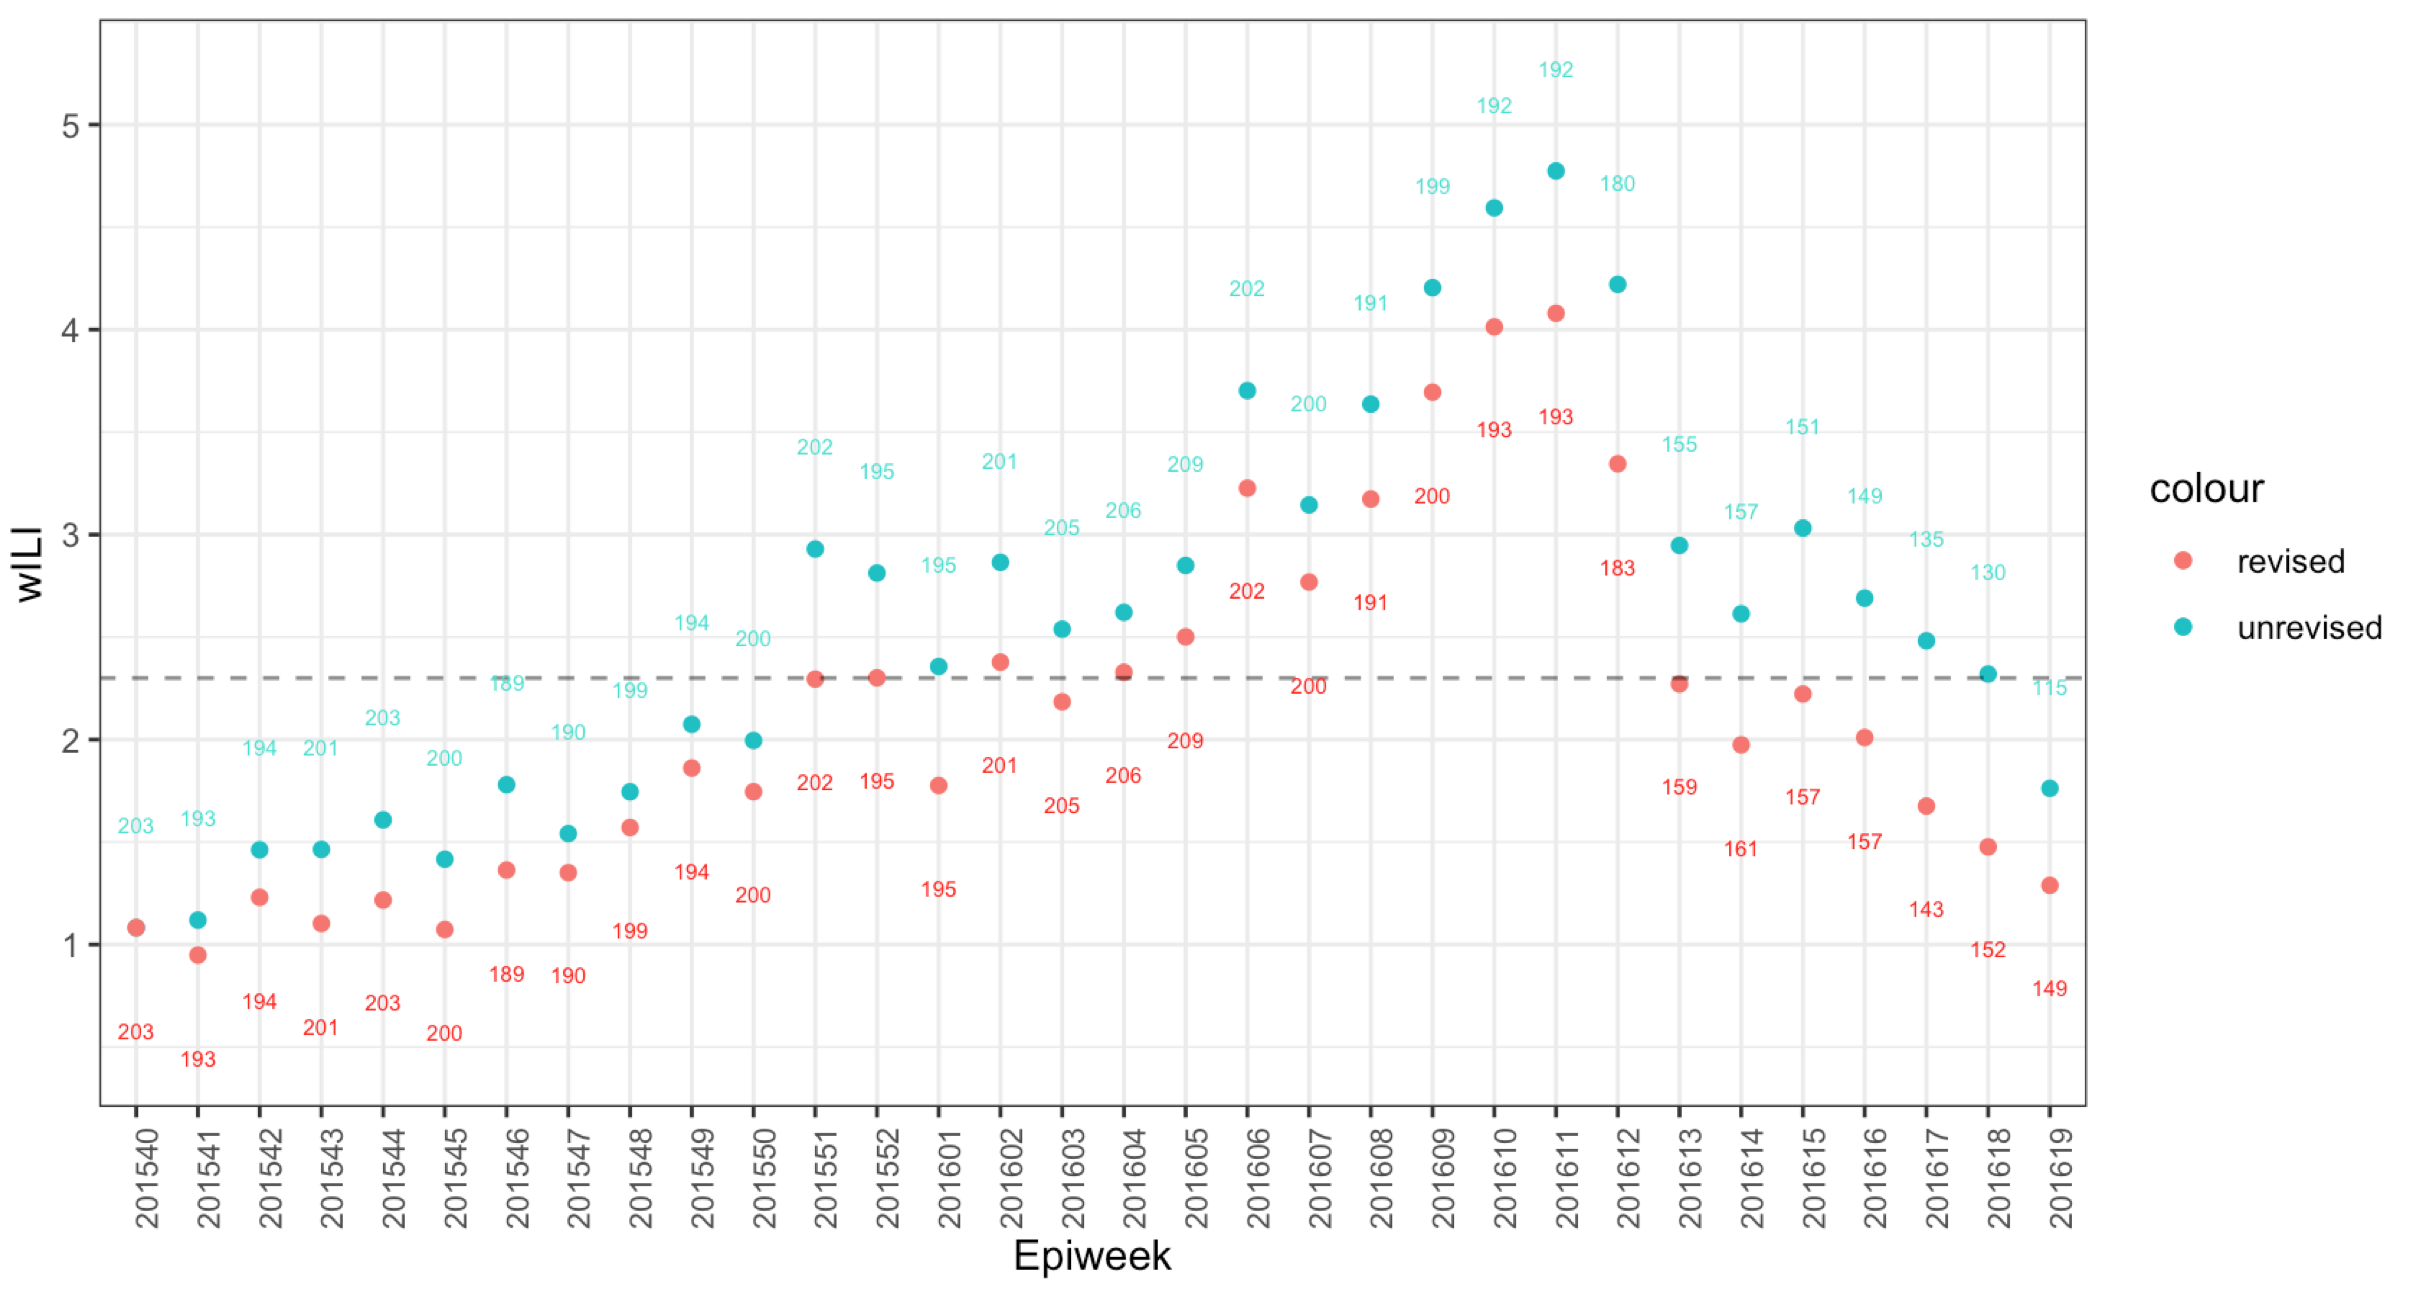
\includegraphics[scale=.35]{same_prov_diff.png}
    \caption{Available wILI data for HHS Region 2 as of epiweek 201615. Notice that even though all providers have reported their data for epiweek 201551, there is still a large difference between the available wILI value and the final wILI value. This is because providers that have already reported are updating their estimates.}
    \label{fig:same_prov_diff}
\end{figure}


Both of these revision mechanisms lead to a significant difference between the available wILI (ILI) and the final wILI (ILI). This is evident in \ref{fig:total_diff}, where we see considerable differences in the available data and the final data. Only $67\%$ of initially reported ILI is within .1 units of the finally observed value.  

%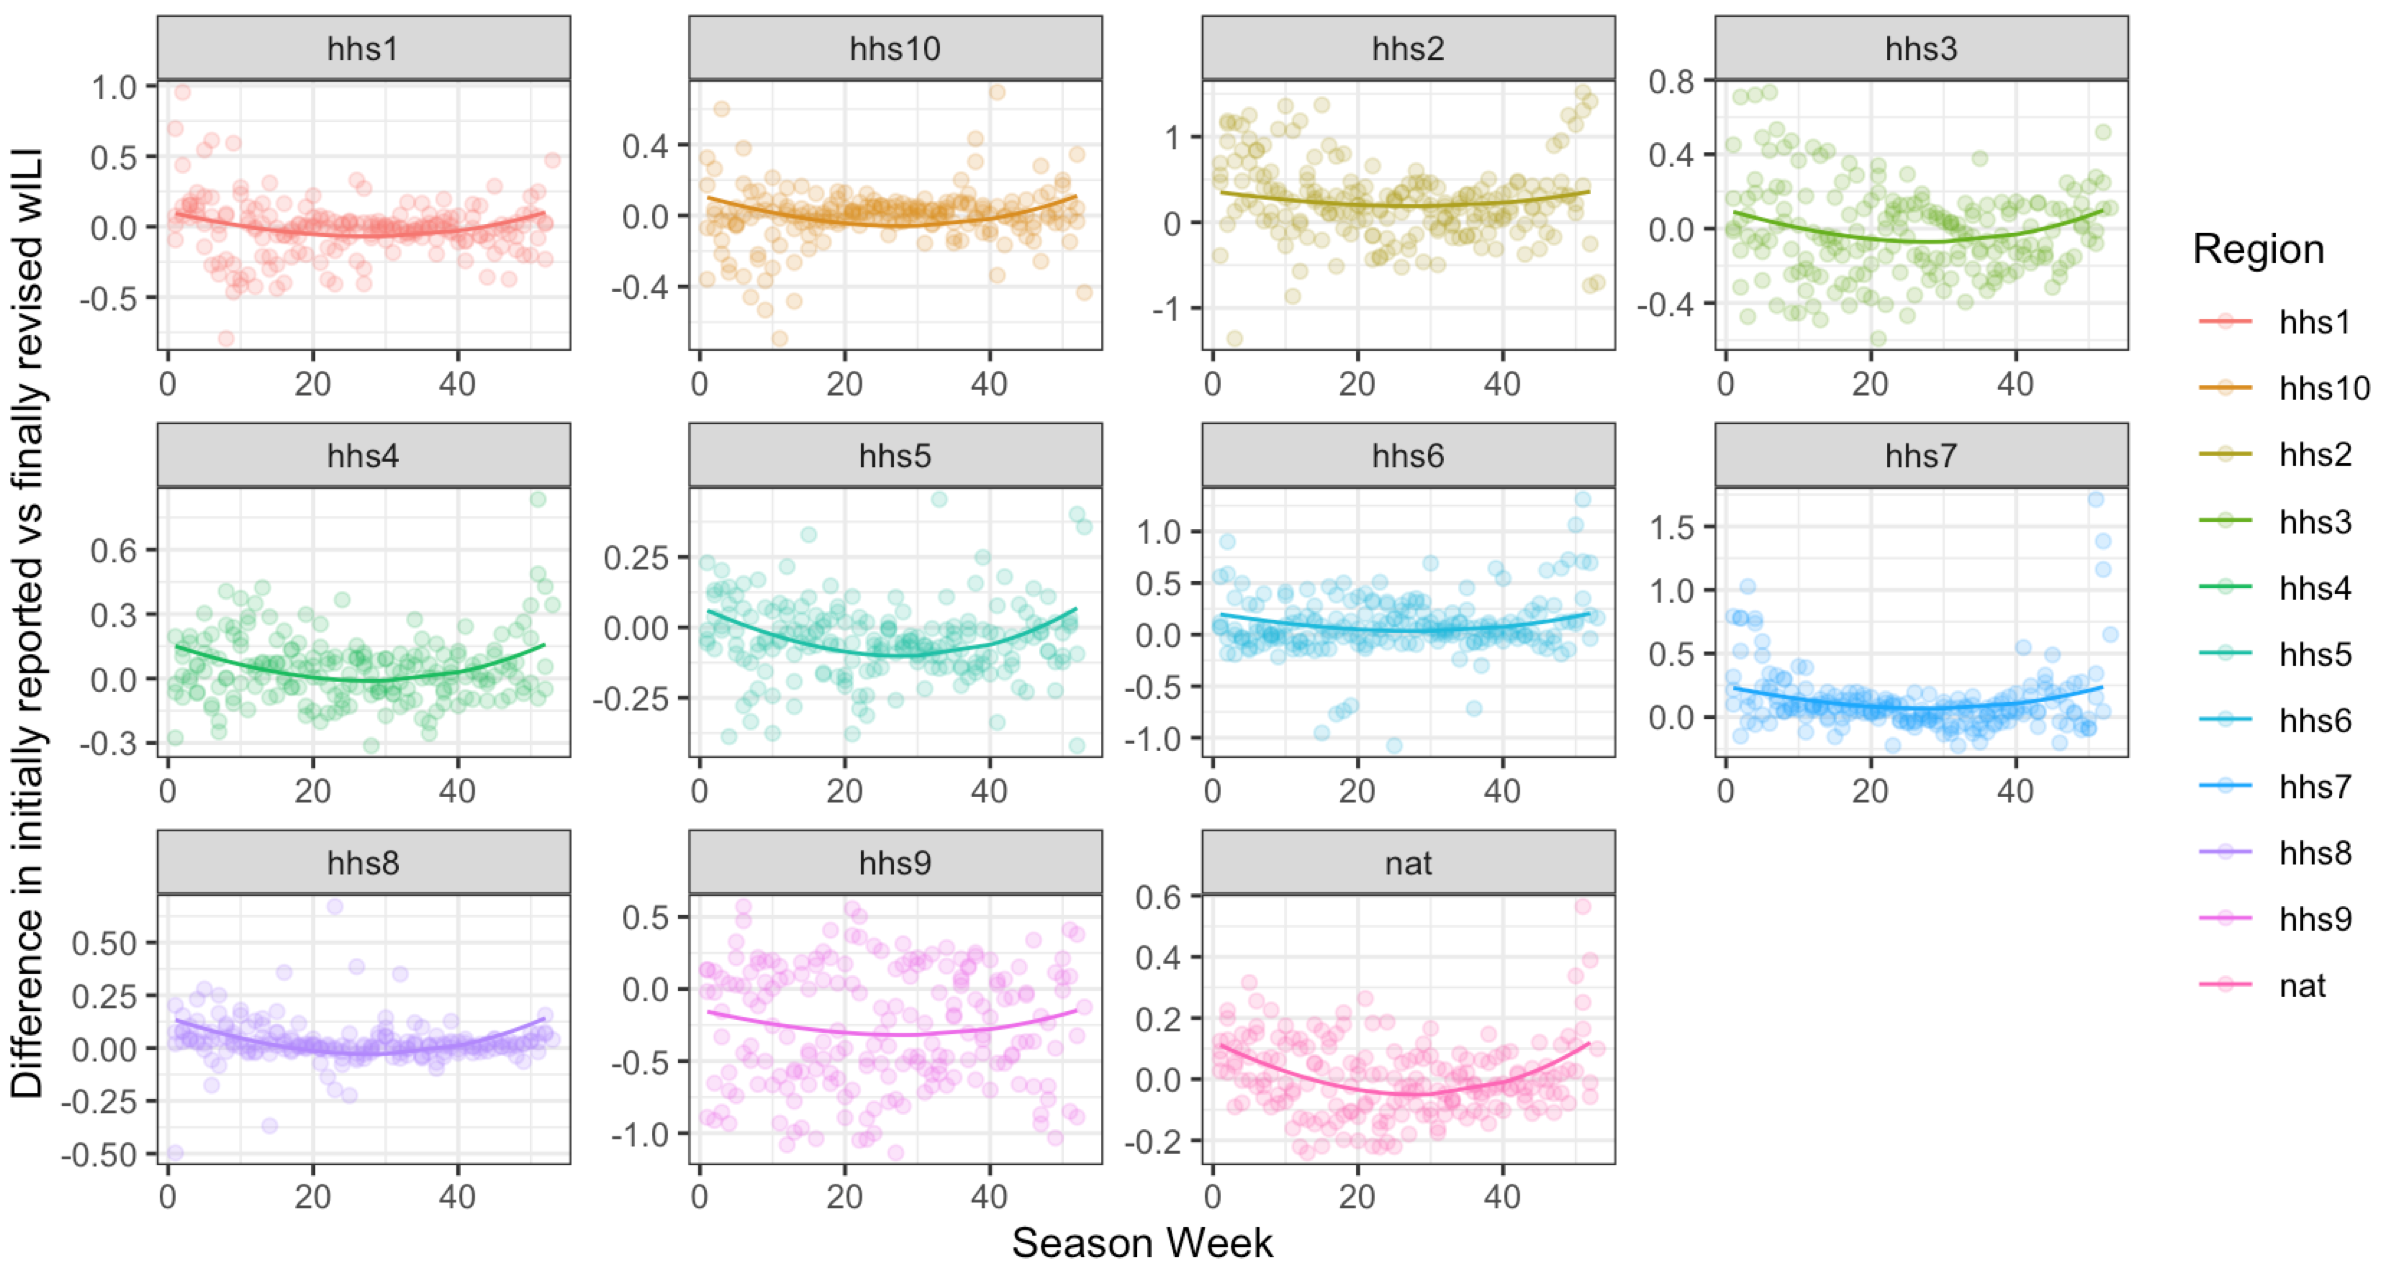
\includegraphics[scale=.25}{CA_rep_diff.png}

Unfortunately, the effects of reporting revisions are magnified during the peak weeks of the season, when accurate estimates of wILI (ILI) are most important. This can be seen in 
\ref{fig:peak_week_revisions}, 




\section{Modelling revisions}

In order to correct for reporting revisions after a forecast has been made, we first define our forecast distribution for a given region $r$, season $s$, epiweek $w$, step ahead $h$ and model $m$ as $P_{r,s,w,h,m}$. This uniquely defines a forecast distribution submitted to the FluSight challenge. 

However, this distribution was produced under the presence of reporting revisions, meaning the data used to forecast was not completely reported. To correct for this we first estimate the revised ILI value at epiweek $w$ and compute the difference between the observed value at epiweek $w$. We refer to this estimated difference as $d_{w,r,s}$. 

Once we estimate the difference we can shift our forecast distribution by the estimated difference to produce a new forecast distribution that has accounted for the expected revision to the data. We do this by first sampling from the original forecast distribution, 



\begin{equation}
   x_1,...,x_n \sim P_{r,s,w,h,m}^{original} 
\end{equation}
\begin{equation}
   y_i = x_i + d_{w,r,s}
\end{equation}


which yields the empirical forecast distribution $P_{r,s,w,h,m}^{adjusted}$ of the form
\begin{equation}
  F_{P_{r,s,w,h,m}^{adjusted}}(y) =\frac{1}{n}\sum_i I(y_i < y) 
\end{equation}

We can then compute the forecast skill under both $P_{r,s,w,h,m}^{adjusted}$ and $P_{r,s,w,h,m}^{original}$ across all indices $r,s,w,h,m$ to evaluate the relative performance. 

Finally, in order to estimate $d_{w,r,s}$ we use a regression model of the form


\begin{equation}
    d_{w,r,s} = \beta_0 +\beta_1 S(w) + \beta_2 r + \epsilon 
\end{equation} 

    $$\epsilon \sim N(0,\sigma^2)$$

where $w$ is epiweek (40-52,1-20), $r$ is region and $S(w)$ is a spline function. 

\begin{figure}
    \centering
    \includegraphics[scale=.35]{model_fit.png}
    \caption{Model fits to the difference between initially reported wILI and finally revised wILI ($d_{r,s,w}$) for 2012/2013-2016/2017 seasons stratified by region. }
    \label{fig:my_label}
\end{figure}
\section{Experimental Setup}

In order to evaluate the effects of reporting revisions in a model agnostic way. We borrow from Gibson et. al and sample from the set of forecast distributions made publicly available by the CDC \cite{cdcfluepi}. This allows us to generate the forecast distribution $P_{r,s,w,h,m}$ as above. 

We train the revision model in Equation 7 on data from 2012/2013 through 2016/2017 and reserve 2017/2018 through 2018/2019 as test seasons to evaluate our model under single-bin scoring. 

We compare the forecast skill of the delay adjusted distributions against the original distribution for all regions and epiweeks in the test seasons.
\section{Results}

Under the mean revision model we are able to improve $93\%$ of models by an average of $.00227$ skill units. This is demonstrated in 
\begin{figure}
    \centering
    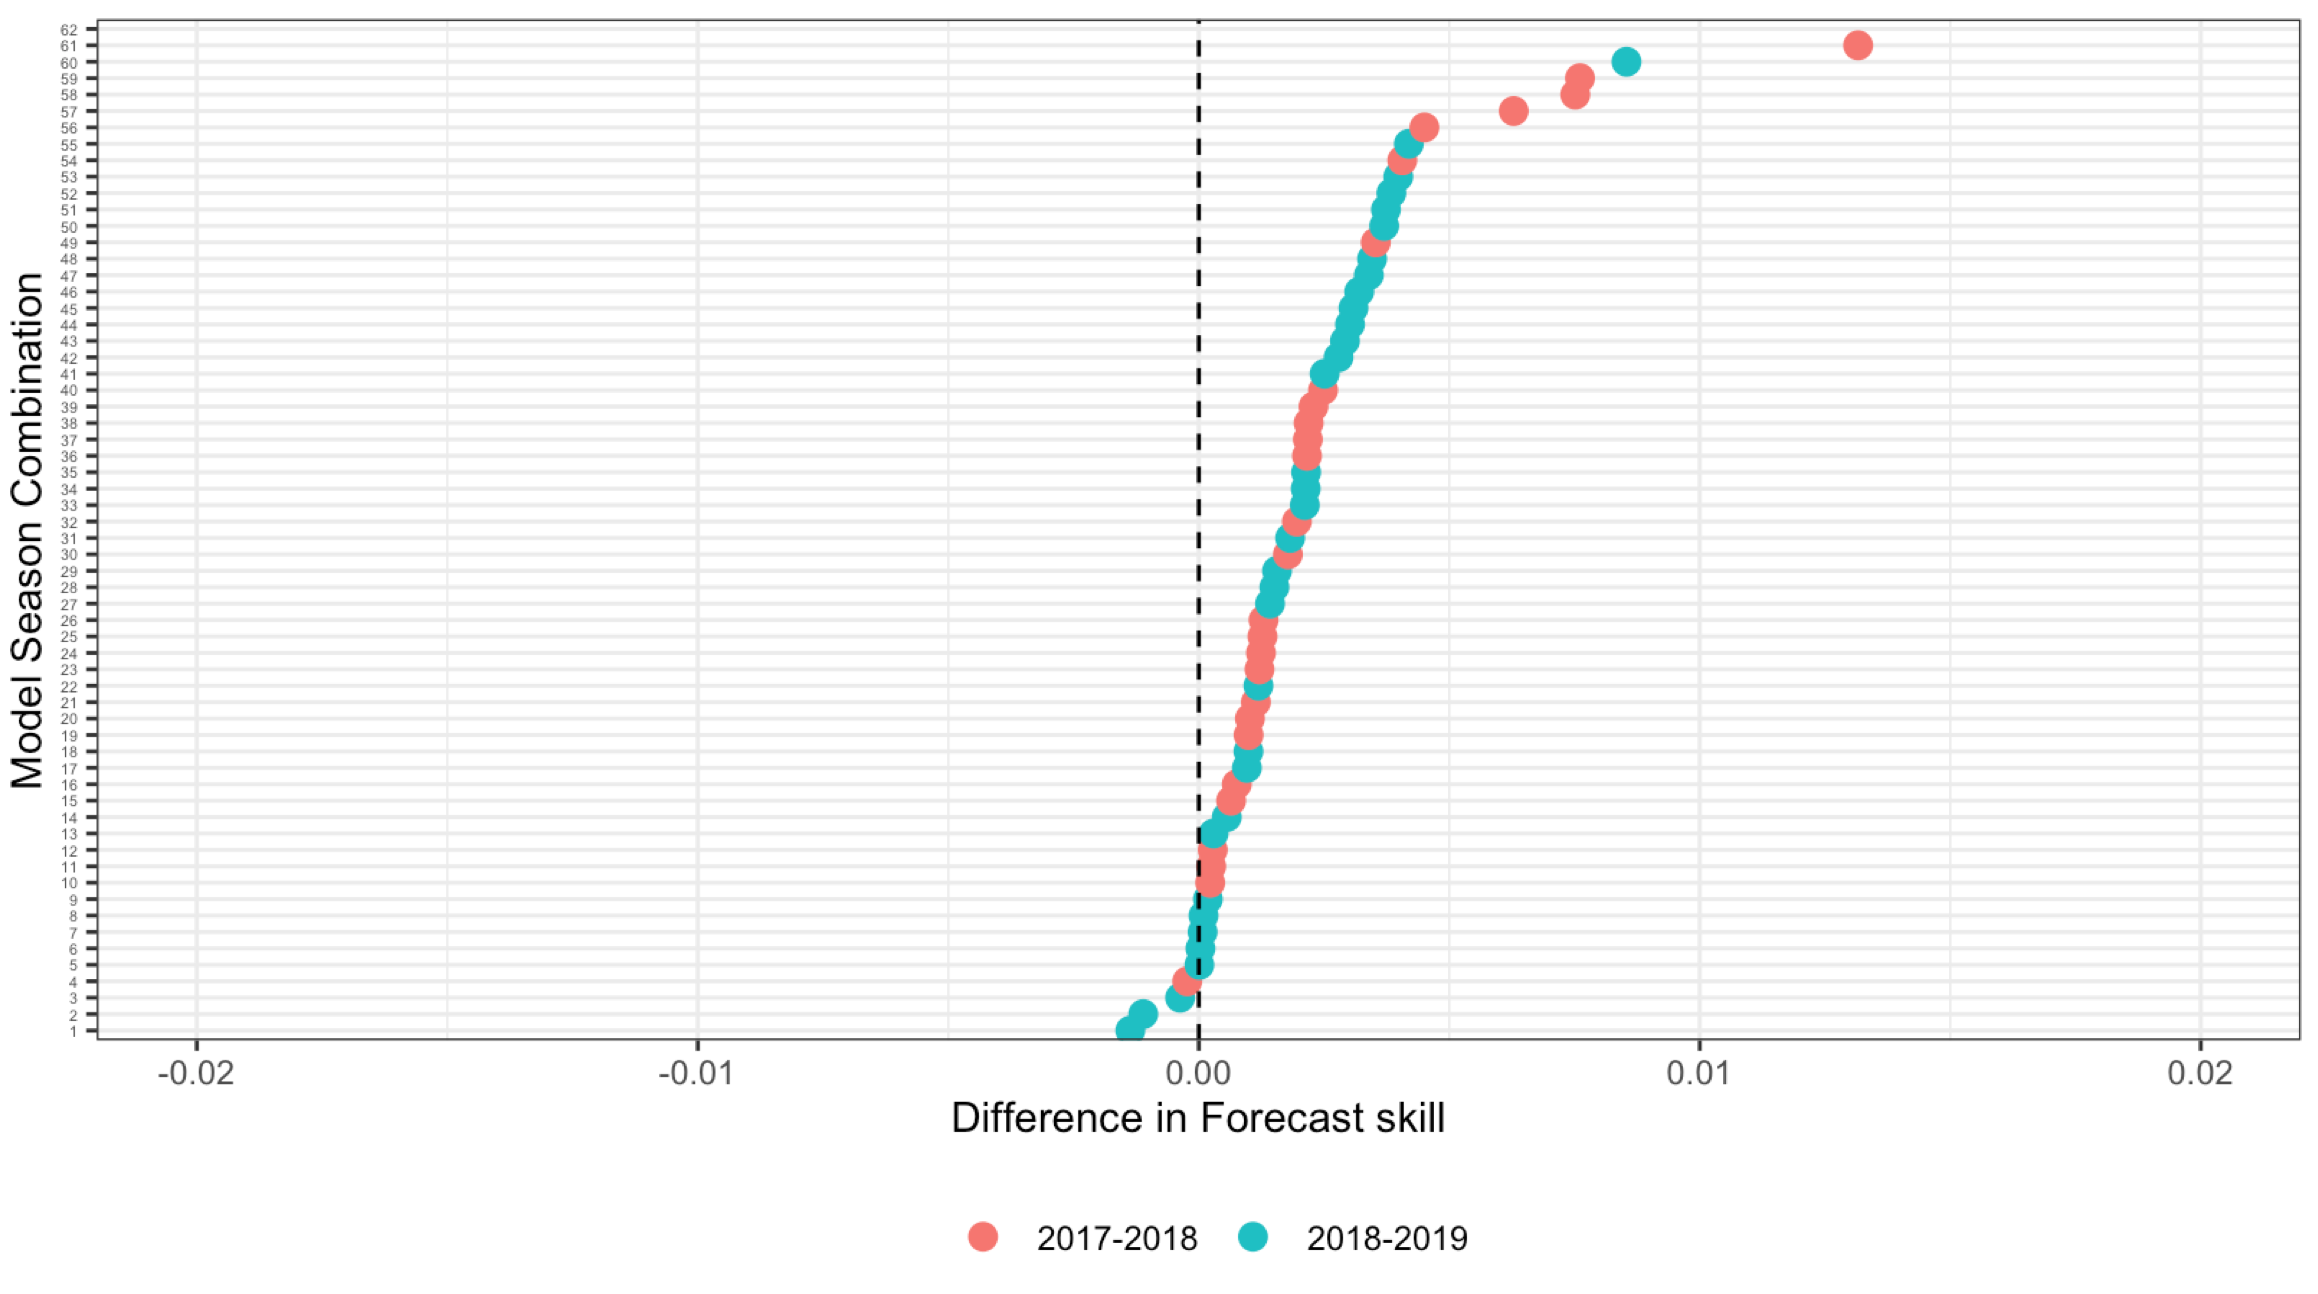
\includegraphics[scale=.3]{percent_improvement.png}
    \caption{Difference in forecast skill between delay adjusted and original forecast submissions.  }
    \label{fig:my_label}
\end{figure}



\begin{figure}
   \begin{subfigure}{.5\textwidth}
  \centering
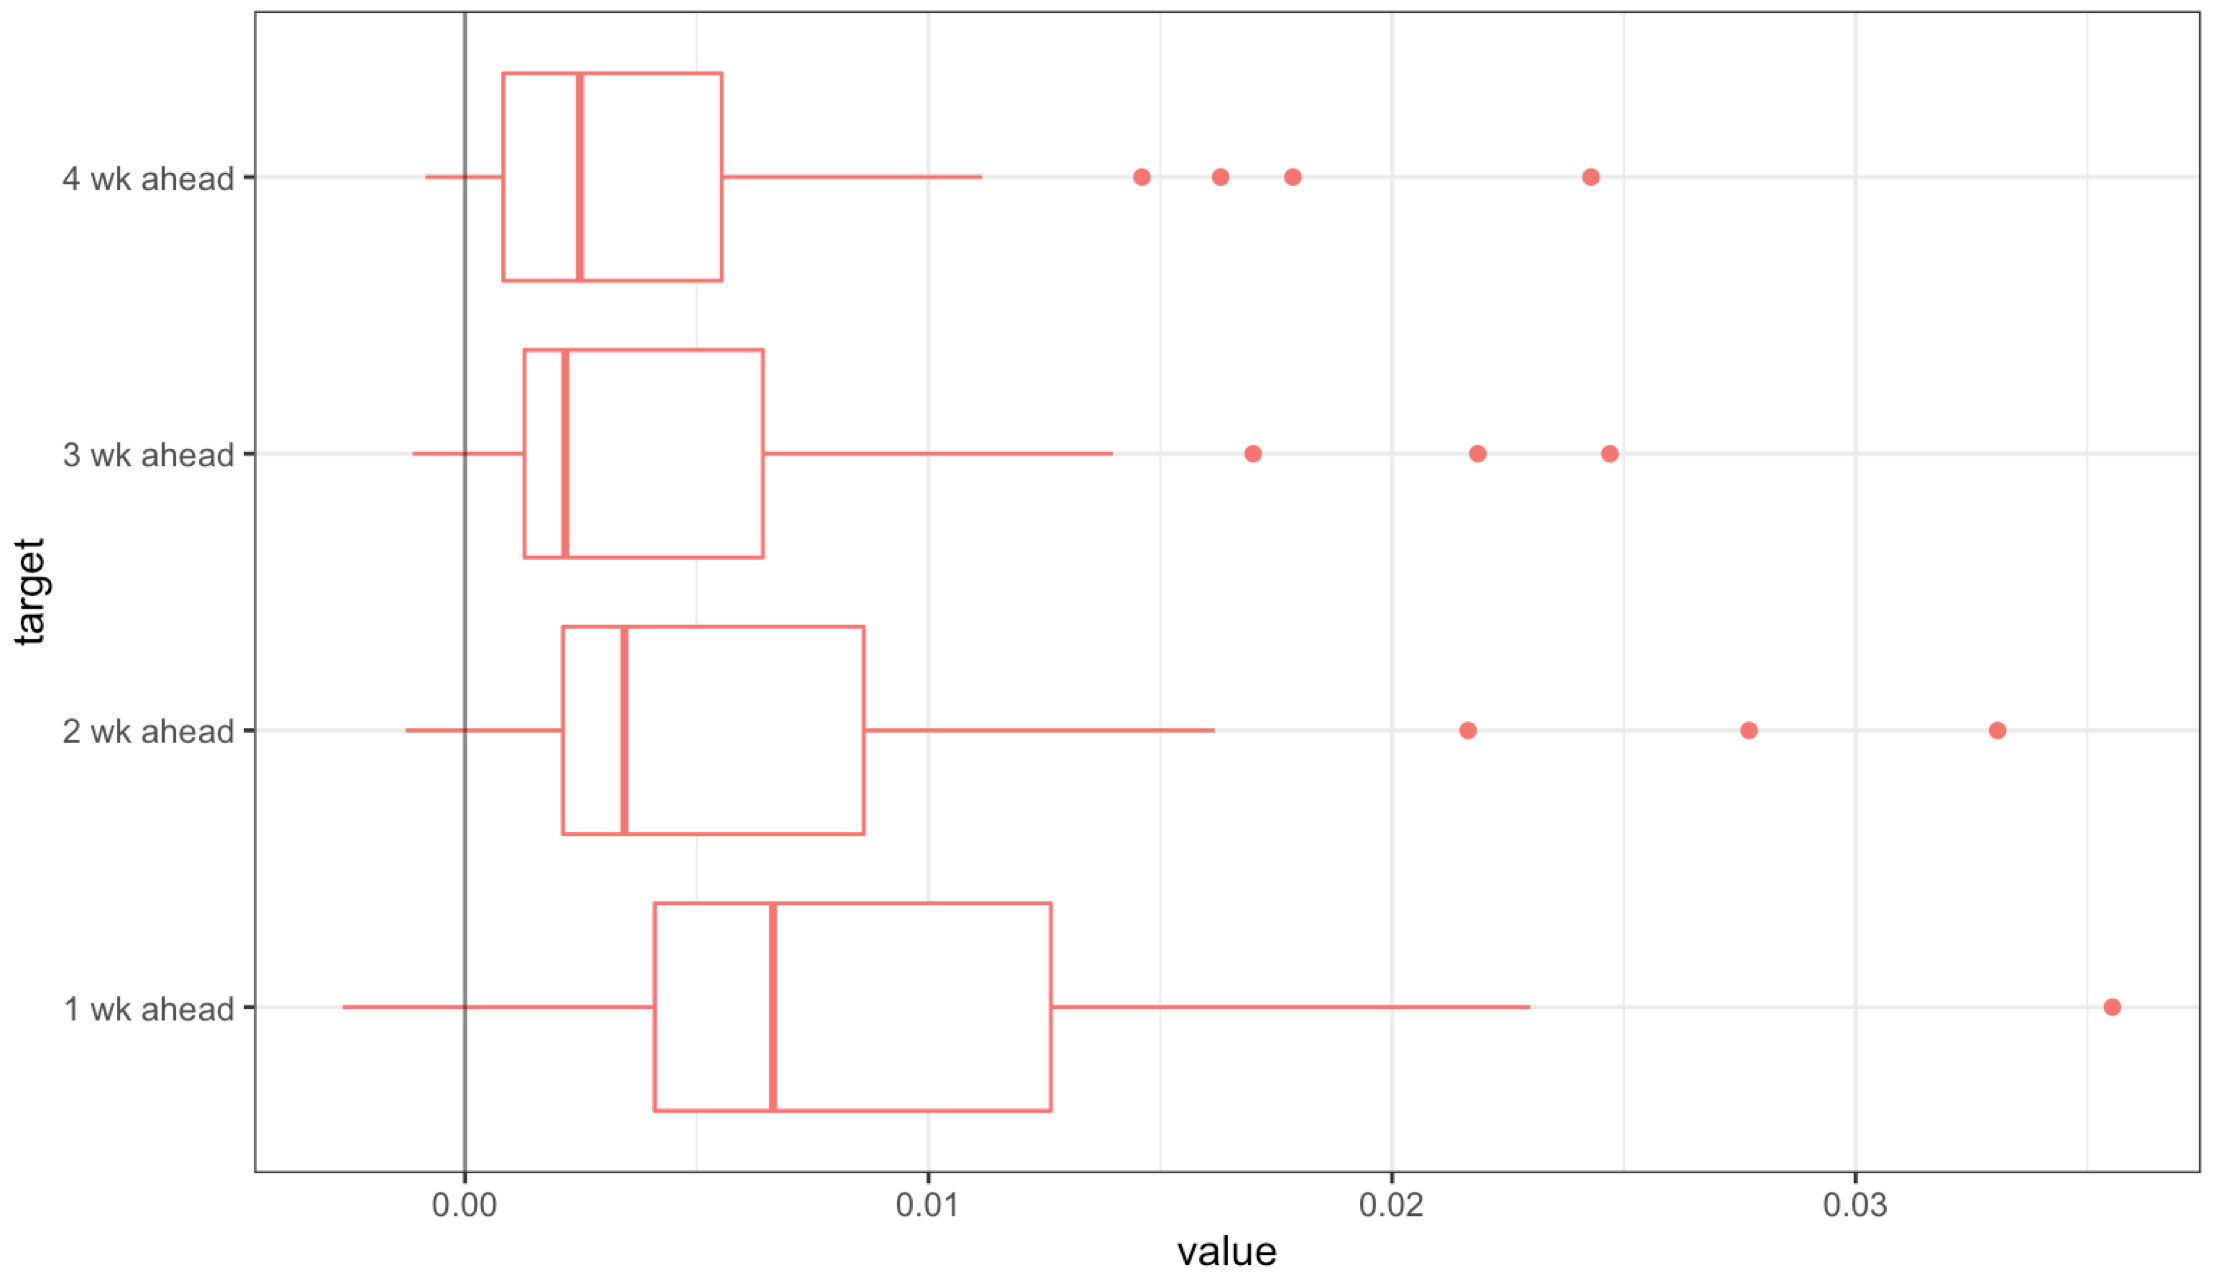
\includegraphics[scale=.15]{target_chap2.png}
 \caption{Target}
\end{subfigure}%
\begin{subfigure}{.5\textwidth}
  \centering
    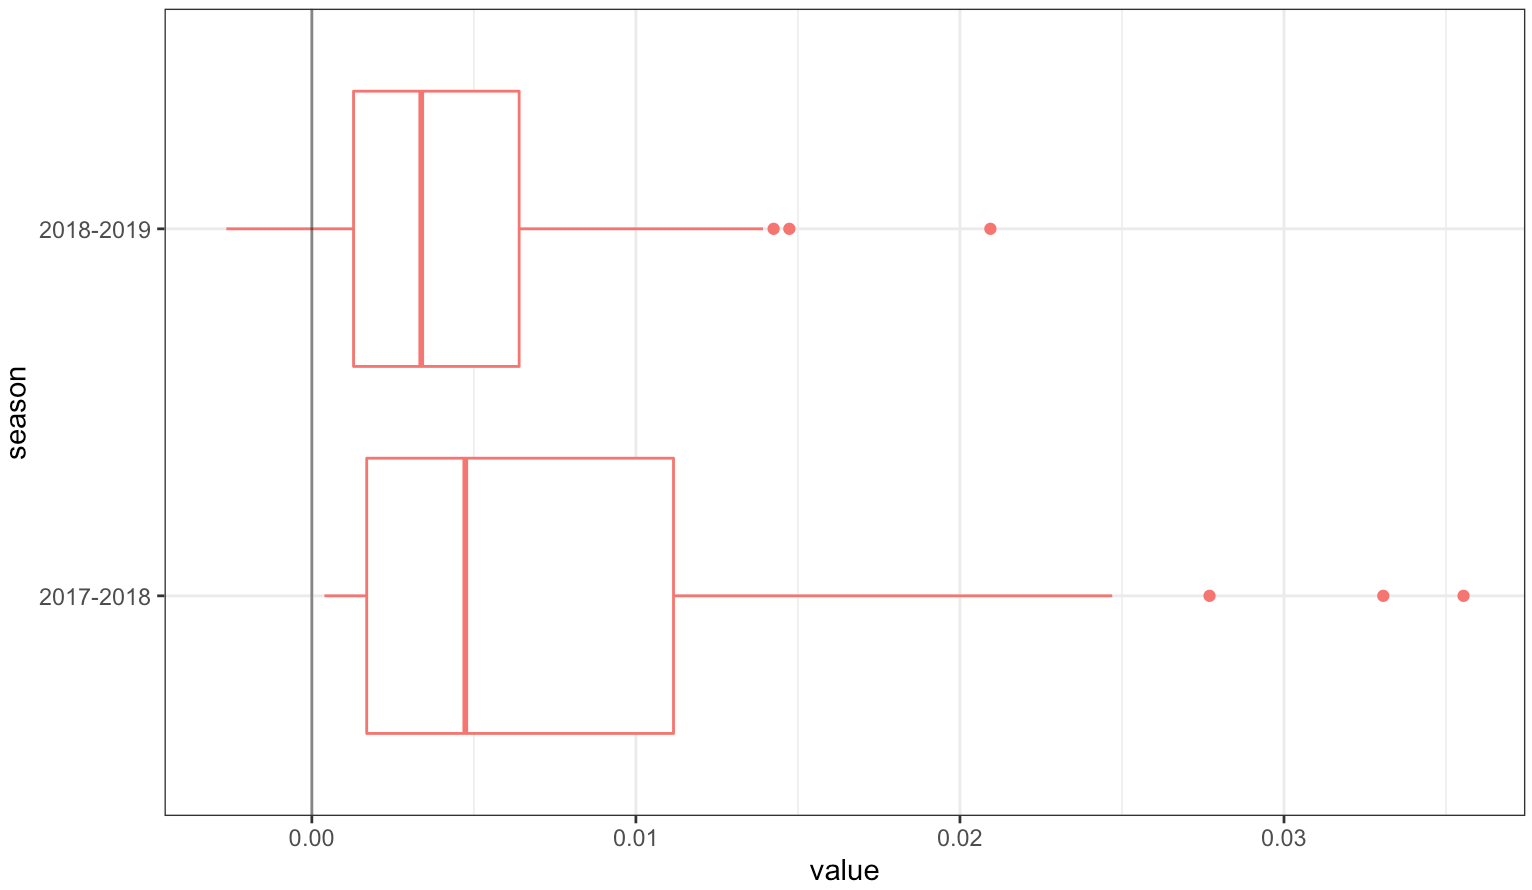
\includegraphics[scale=.2]{season.png}
    \caption{Season}
\end{subfigure}
\centering
\begin{subfigure}{.5\textwidth}
  \centering
    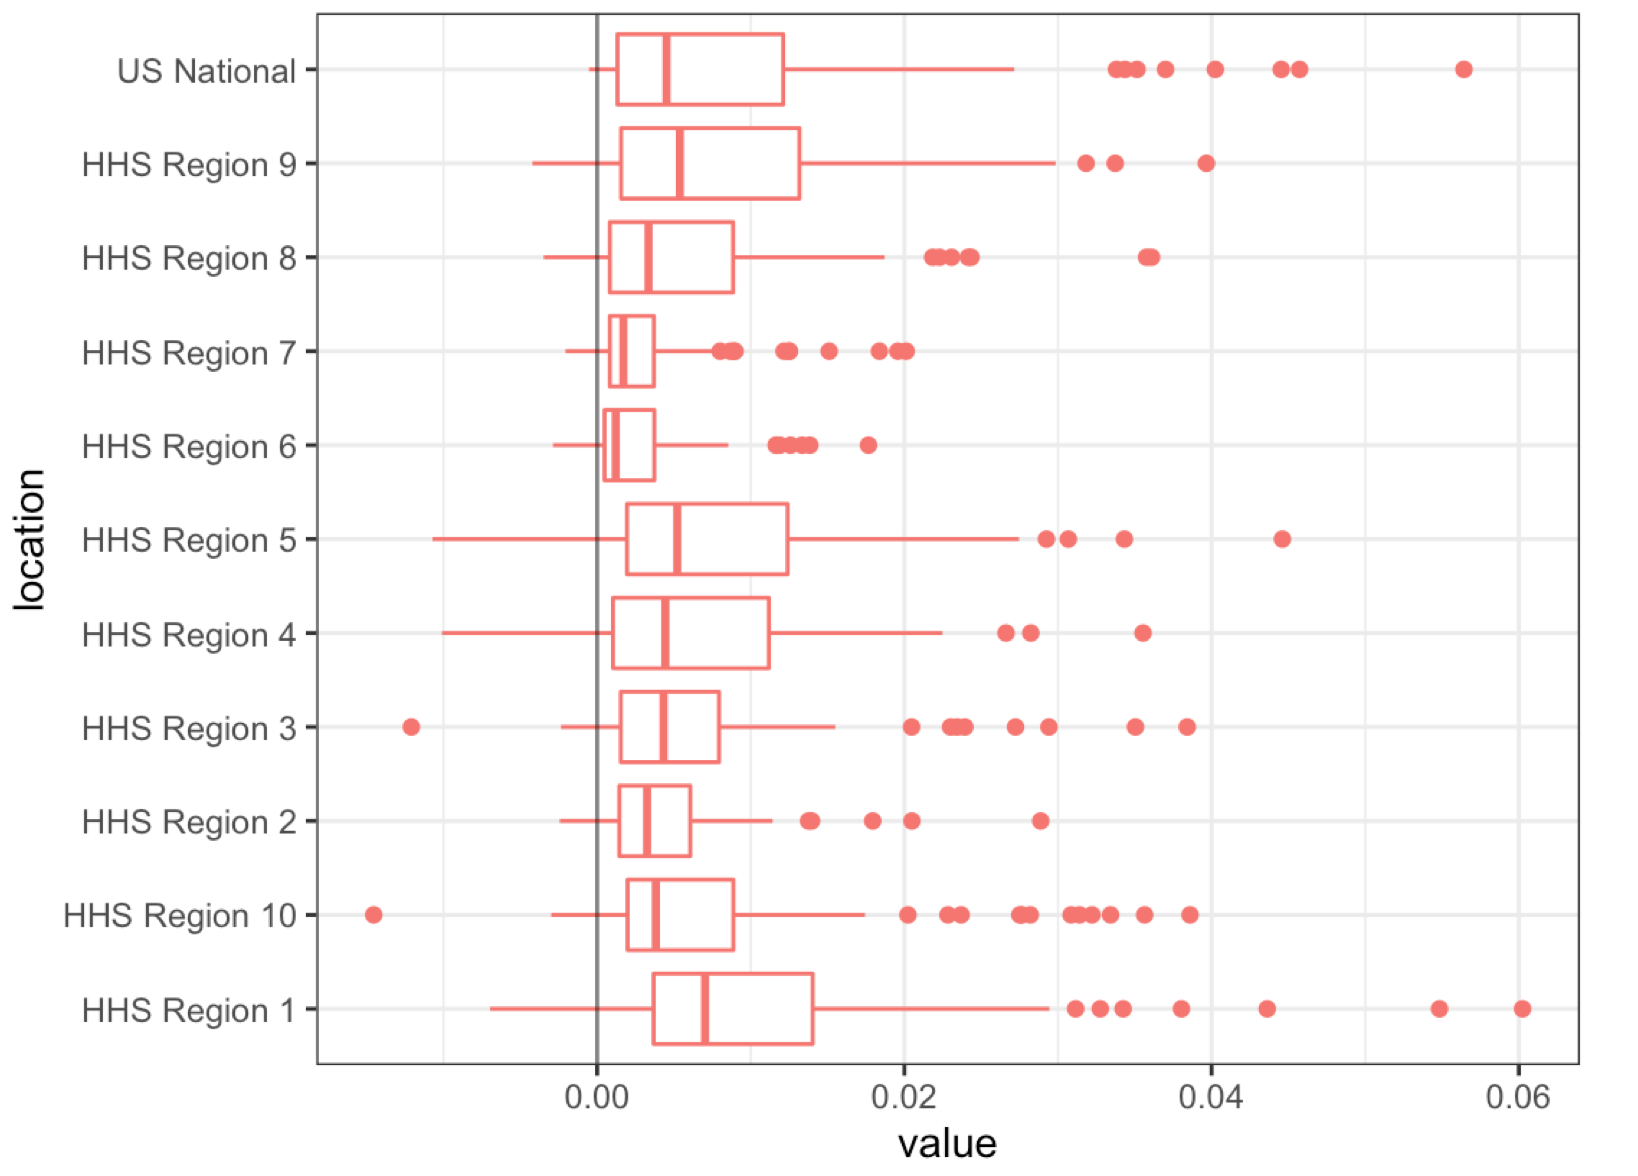
\includegraphics[scale=.3]{region.png}
    \caption{Region}
\end{subfigure}

\label{fig:model_results}
\end{figure}

\section{Conclusion}


Flu forecasting is a challenging but critical endeavour in preparing public health communications at the both the national and state level. Reporting revisions add an additional layer of difficulty in forecasting. Unfortunately, these revisions arise from human behavior, by providers either not reporting in a timely fashion or by simply updating their estimates. This means accounting for reporting revisions is not practical without data at the provider type level. Pushing for greater provider granularity will improve forecasts and lead to more reliable public health actions. 


\chapter{Mechanistic Bayesian Forecasts of COVID19}
%\date{}                                           % Activate to display a given date or no date






The COVID-19 pandemic emerged in late December 2019. In the first six months of the global outbreak, the US reported more cases and deaths than any other country in the world. Effective modeling of the course of the pandemic can help assist with public health resource planning, intervention efforts, and vaccine clinical trials. However, data quality during a pandemic suffers from under-reporting, delayed reporting due to reporting infrastructure issues, and limited testing. Traditionally, compartmental models have been used to model emerging pandemics. However, the basic compartmental framework is difficult to operationalize in a complex data environment. We propose a novel Bayesian compartmental model (MechBayes) that builds upon the classic compartmental framework of susceptible-exposed-infected-recovered (SEIR) model to operationalize COVID-19 forecasting in real time. This includes non-parametric modeling of varying transmission rates, non-parametric modeling of case and death discrepancies due to testing and reporting issues, and finally joint observation likelihood on new case counts and new deaths. The model has been used to submit forecasts to the US Centers for Disease Control, through the COVID19-ForecsatHub repository organized by the Reich Lab. We examine the performance relative to a baseline model in addition to performing an ablation test of our extensions to the classic SEIR models. We demonstrate a significant gain in both point and probabilistic forecast scoring measures using MechBayes.
%\begin{itemize}
%\item Covid has affected XX people
%\item Forecasts useful for public health resource planning, intervention planning (vaccine trials), and disease burden
%\item Basic Mechanistic Models unable to capture complexities of real world disease epidemics due to 
%\begin{itemize}
%\item Complexities of interventions 
%\item Issues with testing and reporting
%\end{itemize}
%\item We propose a novel forecasting algorithm to overcome 
%\begin{itemize}
%\item Under-reporting of cases
%\item Time-varying interventions
%\end{itemize}
%\item Bayesian end to end estimation using both cases and deaths in numpyro
%\end{itemize}



%\section{}
%\subsection{}

\section{Introduction}

The emergence of COVID-19 in early 2020 in the United States developed into the largest pandemic the country has seen in over a century. Understanding the future trajectory of the pandemic is crucial for minimizing the impact across the nation in terms of healthcare burden, economic impact, treatments and public health response. Forecasts of incident and cumulative deaths due to COVID may help in resource allocation, vaccine clinical trial planning, and re-opening strategies. Forecasts provide important data to decision-makers and the general public and can improve situational awareness of current trends and how they will continue in coming weeks. 

Infectious disease forecasting, at the time horizon of up to 4 weeks in the future, has benefited public health decision makers during annual influenza outbreaks \cite{lutz2019applying}\cite{myers2000forecasting}.  However, many forecasts of seasonal disease, such as influenza, often rely on ample historical data to look for patterns that can be projected forward into the future. In an emerging pandemic situation, models must be able to fit to limited data. In modeling the COVID-19 pandemic, many research groups have turned to the use of differential equation models to explain the underlying transmission of a disease through a population. First introduced by  Kermack and McKendrick, the model assumes the each individual is in one of a mutually exclusive set of compartments, typically either the susceptible, exposed, infected, or recovered compartment \cite{kermack1927contribution}. The model is specified by setting the rates of flow of individuals between compartments. While these models have been used since their inception in the early 20th century, the COVID pandemic represents a unique opportunity to explore their properties in real-time at both local and global scales.
 
Compartmental models have been used to effectively model and forecast disease in non-pandemic situations both retrospectively and in real-time. These include complex compartmental models for real-time influenza forecasting \cite{shaman2012forecasting}\cite{osthus2017forecasting}\cite{ong2010real}, even including a retrospective model evaluation of the 1918 influenza pandemic \cite{hall2007real}. Compartmental models have been used not just in respiratory disease but in Ebola \cite{lekone2006statistical}, measles \cite{bokler1993chaos}, dengue \cite{syafruddin2012seir} and a wide variety of other diseases

In this work, we introduce a novel operational forecast model based on mechanistic foundations and tailored to the particular needs and data availability of COVID-19. These include, but are not limited to, severe under reporting of cases due to low testing rates especially in mild or asymptomatic cases, time-varying testing rates, delayed reporting, and both the addition and removal of control measures such as social distancing, lockdown, and mask use. We accomplish this by modeling transmission and deviations from cases and deaths (beyond the case fatality ratio) non-parametrically. Our observation model is able to handle case data which is reported as new cases, instead of prevalent, and new deaths, instead of cumulative. We choose a Bayesian framework that allows for uncertainty in the epidemiological parameters that are unidentifiable from the data, introducing flexibility suited to forecasting. Implementation in a Bayesian framework also allows for use of a cutting edge probabilistic programming framework for speed and rapid model development. 

Our main goal in developing MechBayes is to forecast observed incident deaths, and because we have limited historical data on COVID-19, we think compartmental models are among the most parsimonious models available for forecasting. Our focus is not on identifying internal parameters of the model, many of which are poorly determined or not identifiable from the available data. We are willing to accept biologically unrealistic parameter values or priors for latent variables; but not ones that lead to gross pathologies during inference and forecasting. The non-parametric extensions to the underlying SEIR model also mean that any inference on epidemiological parameters should be carried out very carefully. We distinguish this from scenario projection models, which require well identified epidemiological parameters that can be set to counterfactual values under different scenarios, such as an increase or decrease in intervention levels. 


 We demonstrate the success of the model in both forecast submissions to the US Centers for Disease Control via the COVID-19 Forecast Hub as well as an ablation model comparison to demonstrate the additional forecast accuracy of our extensions beyond the basic SEIR model. In what follows we first describe the available data and forecast submission infrastructure, outline the basic SEIR compartment model, describe our extensions for real-world pandemic forecasting, and finally evaluate the model using both real-time evaluation from submissions and a retrospective model component analysis. 



\section{Related Work}


Compartmental models have also been adopted into a Bayesian framework before, including both stochastic disease dynamics and deterministic dynamics \cite{hotta2010bayesian}\cite{dukic2012tracking}. Non-parametric transmissibility was included in a Bayesian SEIR model to study Ebola by Frasso and Lambert \cite{frasso2016bayesian}. Time-varying transmissibility has also been studied in the frequentist setting using complex non-parametric functions \cite{smirnova2019forecasting}. Many efforts have been made to use SEIR models in forecasting COVID-19 \cite{giordano2020modelling}\cite{yang2020modified} \cite{bertozzi2020challenges}\cite{prem2020effect}\cite{flaxman2020estimating}.

With the outbreak of COVID-19, accounting for testing has become a critical element in effectively using an SEIR model. Lopez et al. used a fixed case and death deviation model to model undiagnosed individuals in Spain and Italy \cite{lopez2020modified}.  Perhaps the most similar model to ours was put forth by Pei et al. \cite{pei2020differential}. This model was an extension to the SEIR model with time varying transmission and case and death deviation model. However, their model fixed case and death deviation model across time and was fit using Kalman Filter techniques instead of Bayesian HMC. They also used the model mostly for counterfactual scenario projections instead of forecasting. Models that have accounted for time-varying testing have mostly used the renewal style equations \cite{abbott2020estimating}\cite{flaxman2020estimating}. These models do not use a differential equation model as the core component, but rather parameterizes new cases as a function of the time varying reproduction number and the serial interval. 


\section{Data}
	In this analysis we used confirmed case counts and deaths as reported by the Johns Hopkins University Center for Systems Science and Engineering \cite{dong2020interactive}. This a time series dataset which we truncate to begin March 1st 2020 to August 1st 2020 and captures all 50 states, as well as Guam, Puerto Rico, American Samoa, District of Columbia, Northern Mariana Islands and U.S. Virgin Islands. As noted in \cite{krantz2020level}, COVID-19 cases are under-reported, with the fraction of all infections reported as cases for the U.S. estimated at 20-30\% \cite{russel2020using}. 
		There are large discrepancies in reporting practices across the states (Figure \ref{fig:data}). For example, New Jersey reported an additional 1600 incident deaths when changing reporting practices to include ``probable" deaths as well as confirmed deaths due to COVID-19 on June 25th 2020. However, many other states have at least one outlying value, usually due to delayed reporting, where a large number of deaths occurring in previous weeks are reported on a single day. We can also see from Figure \ref{fig:data} that some states do not report on particular days (usually weekends) leading to 0 incident deaths for the day. Some states also revise the cause of death, allowing for negative incident deaths.  Some states exhibit relatively regular weekly reporting cycles, with reporting dropping off significantly on the weekends. This effect is most pronounced at the aggregate U.S. level, which shows a clear weekly cycle in reporting. 
	
	
We made probabilistic forecasts  for 1-4 week ahead incident and cumulative deaths for all geographies. An individual forecast distribution is represented by a set of quantiles for incident and cumulative deaths from 1-4 weeks ahead. Since our model produced cumulative forecasts by aggregating incident, we choose to only evaluate incident. The quantiles used are $\mathbb{Q} = {.05,.10,....,.90,.95} \cup {.01,.99}$, with the median ($.5$ quantile) representing the point-forecast. Forecasts were made on Monday evenings and therefore use the incident data up until the Sunday before. A one-week ahead target corresponds to the following Saturday. A two-week ahead corresponds two the next Saturday and so on. Forecasts were evaluated using mean-absolute-error (MAE) and empirical coverage probability at the 95\% level. This allows us to assses both point prediction and calibration of forecasts.



 \begin{figure}
     \centering
     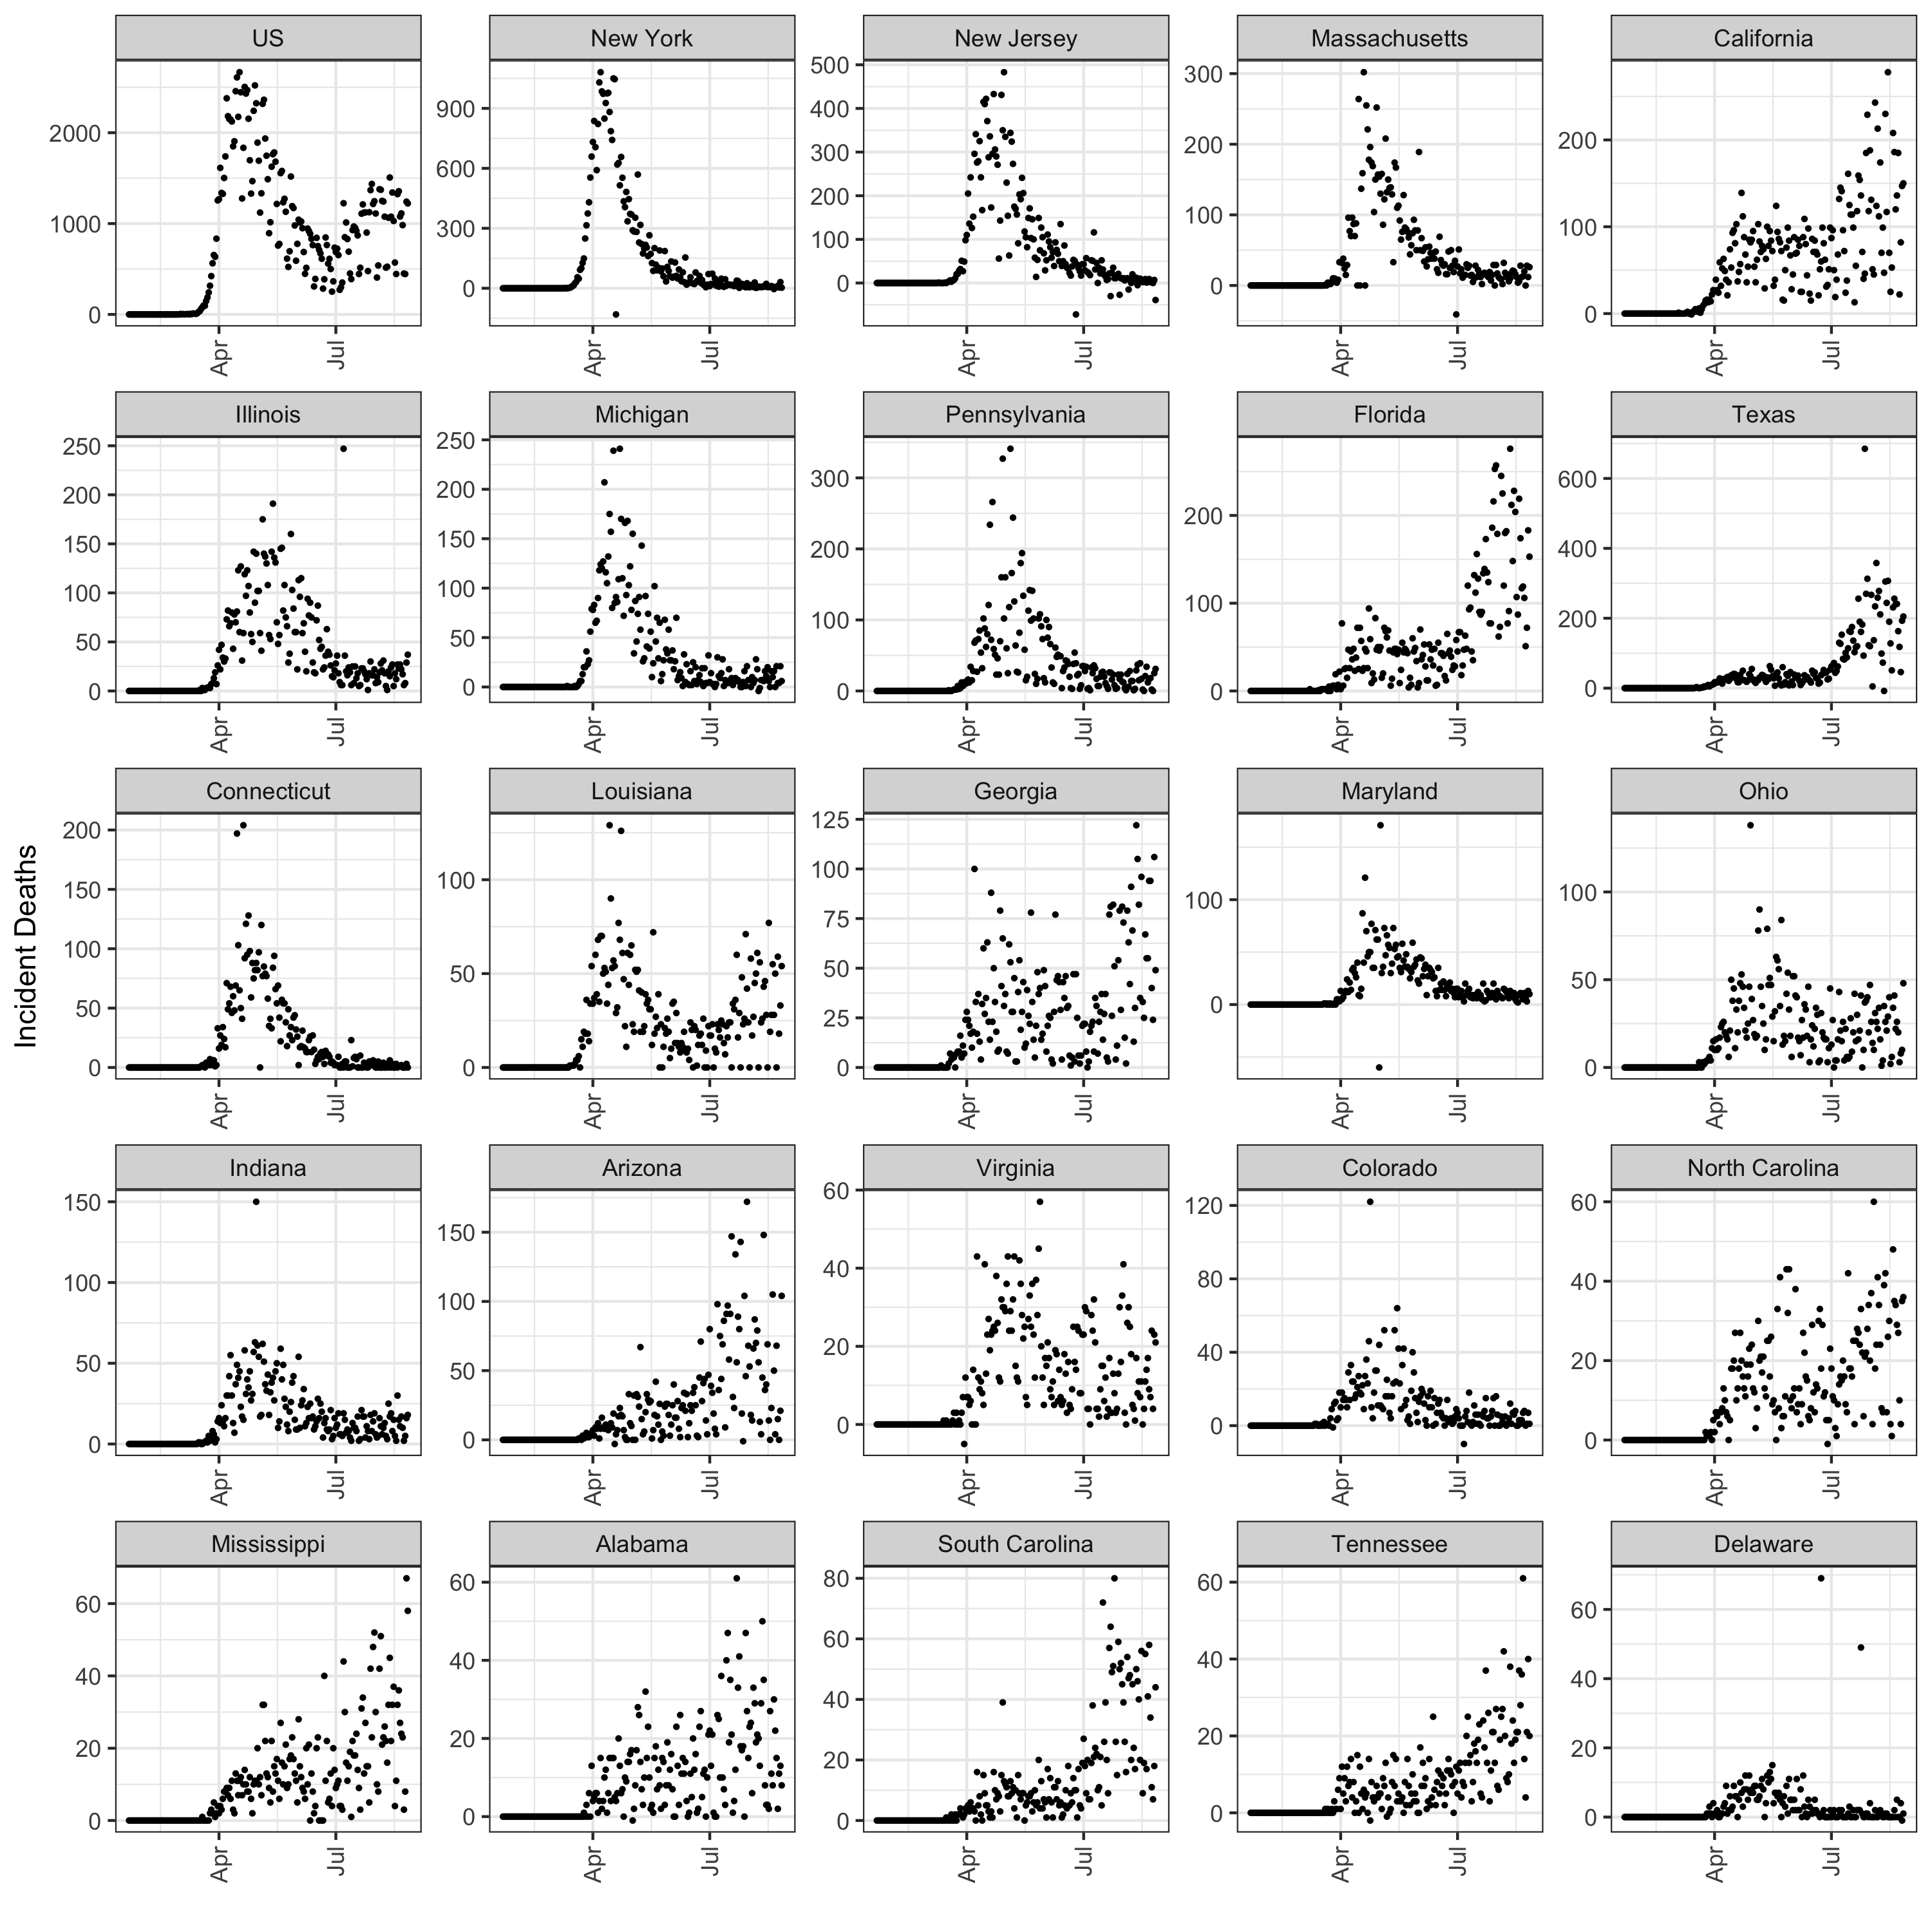
\includegraphics[scale=.14]{data_plot.png}
     \caption{Deaths by state for any state with over 50 incident deaths for a given day. Notice the large variability in incident reporting. There are significant delayed reporting, with New Jersey reporting over 1500 backlogged deaths when switching to include ``probable" deaths. In some states, there appears to be a weekly cycle where deaths are under-reported on the weekend. This is especially pronounced for the U.S. as a whole. We can also see that there are some negative incident deaths, where data are revised to account for deaths that were incorrectly attributed to COVID-19. }
     \label{fig:data}
 \end{figure}
 
 \section{Compartmental Model}

In a given time-step (e.g. one day), each member of the population of a single geography belongs to one of the following mutually exhaustive compartments:
 susceptible $S$, exposed but not yet infectious $E$, infectious $I$, recovered $R$, hospitalized before death $D_1$, and deceased $D_2$ (Figure \ref{fig:seird}). Here we assume everyone who is hospitalized will eventually become deceased in order to separate the rate of flow into both a case fatality ratio (CFR) parameter as well as a time from symptoms to death parameter, which both have prior estimates from the literature \cite{russell2020estimating}. We omit an explicit hospitalization compartment since the available hospitalization data is highly variable by state and suffers even more reporting issues than case data.  For simplicity, we assume a closed population of size $N$. 
The following parameters govern how members of the population move between compartments:  
\begin{packed_item}
\item $\beta(t)$: transmission rate, which we allow to vary by time $t$
\item $\sigma$: rate of transition from the exposed state $E$ to infectious state $I$; i.e., $1/\sigma$ is the expected duration of the time between exposure and symptom onset. 
\item $\gamma$: rate of transition from  the infectious state $I$ to no longer being infectious (either to state $D_1$ or $R$); i.e., $1/\gamma$ is the expected duration of the infectious period
\item $\rho$: fatality rate (i.e., probability of transitioning from I to $D_1$ instead of I to R)
\item $\lambda$: rate of transition from $D_1$ to $D_2$ 
(i.e., the inverse of expected number of days in $D_1$ compartment before death) 
\end{packed_item}
For a given time-step $t$, the following differential equations describe the changes in each compartment:

\begin{equation}
\begin{aligned} 
\frac{dS}{dt} &= - \beta(t) \frac{SI}{N} \\
\frac{dE}{dt} &= \beta(t) \cdot \frac{SI}{N} - \sigma E \\
\frac{dI}{dt} &= \sigma E - \gamma I\\ 
\frac{dR}{dt} &= (1-\rho)\gamma I \\
\frac{dD_1}{dt} &= \rho \gamma I - \lambda D_1\\
\frac{dD_2}{dt} &= \lambda D_2\\
\frac{dC}{d} &= \sigma E
\end{aligned}
\end{equation}

Here, we include the $C$ compartment to be able to observe the cumulative count of new infections. This captures only the flow into $I$.

We can write this in a state space representation as follows: \[
X(t) = (S(t), E(t), I(t), R(t), D_1(t), D_2(t), C(t))
\]
The update from time $t$ to time $t+1$ can be solved numerically as
\begin{equation}
\bm{X}(t+1)= \text{RK4}\left(\bm{X}(t),\frac{dX}{dt},\beta(t)\right)
\end{equation},
where RK4 is the Runge-Katta 4th order approximation \cite{phan2019composable}.


\begin{figure}
 \begin{center}
\begin{tikzpicture}[node distance=1cm,auto,>=latex',every node/.append style={align=center},int/.style={draw, minimum size=1cm}]
    \node [int] (S)             {$S$};
      \node [int,right=of S] (E)  {$E$};
    \node [int, right=of E] (I) {$I$};
        \node [int, above=of E] (C) {$C$};

    \node [int, right=of I] (D_1) {$D_1$};
    
    \node [int, right=of D_1] (D_2) {$D_2$};
     \node [int, below=of I] (R) {$R$};

   % \coordinate[right=of ] (out); %
    \path[->, auto=false] (S) edge node[yshift=12pt] {$\beta(t) I$ \\[.2em]} (E)
                          (E) edge node[yshift=5pt] {$\sigma$       \\[.2em] } (I) 
                           (E) edge node[yshift=-12pt,xshift=5pt] {$\sigma$       \\[.2em] } (C) 
                           (I) edge node[yshift=5pt] {$\rho\gamma$       \\[.2em] } (D_1)
                           (I) edge node[xshift=30pt,yshift=-5pt] {$(1-\rho)\gamma$       \\[.4em] } (R)
                            (D_1) edge node[yshift=5pt] {$\lambda$       \\[.2em] } (D_2)  ;
                          \end{tikzpicture}
\end{center}
      \caption{Comparmental model parameters }
     \label{fig:seird}
 \end{figure}
 
 
 
 

 
 \subsection{Time-varying transmission parameter}
 
We have seen significant efforts to control the spread of COVID through non-pharmaceutical interventions. These include social distancing, lock-downs, and mask wearing. To add to the complexity, these interventions have been implemented and repealed at different time points. They also face compliance issues \cite{simonov2020persuasive}. In order to capture the aggregate effect of the interventions non-parametrically we choose a flexible model for the time-varying transmission parameter.
We allow $\beta(t)$ to vary as follows, 

\begin{equation}
log(\beta(t)) \sim N(log(\beta(t-1), \sigma_{\beta}^2)
\end{equation}

This model assumes that forecasts are made on the current level of interventions because $\mathbb{E}[log(\beta(t+1))] = log(\beta(t))$. That is, the expected value of a random walk in the forecasting stage is the estimated value at the final time point of available data.

However, this non-parametric model is particularly susceptible to noise in reporting of cases, since $\beta(t)$ is the parameter that takes individuals from $S$ into $E$. To avoid instability issues, especially when forecasting, we smooth each posterior sample of $\beta$ to be the average over the last 10 days from the sample. This is a large enough window to smooth over most reporting issues (excepting delayed reporting). 

\begin{equation}
\beta^*_{forecast}(t+k) = \frac{1}{10}\sum_{i=0}^{9}\beta^*(t-i)
\end{equation}

where $\beta^*(t)$ denotes a sample from the posterior at time $t$.

% \begin{itemize}
% \item Non-parametrically models time-varying transmissibility through a random walk
% \item Makes forecasts conditional on current level of interventions
% \item Requires no external intervention data to make forecasts 
% \end{itemize}
% 
 \subsection{Observation Model}
 
 The observed data used to fit the model is based on time-series data of incident confirmed cases $Cases_{t}$ and incident recorded deaths $Deaths_{t}$. 
For a given state and day, the change in the  confirmed cases and reported deaths are subset of the cumulative number of new infections $C(t)$ and cumulative number of deaths $D2(t)$, respectively. To handle this, we introduce two additional parameters. First, we introduce a case and death deviation, beyond the case fatality ration, of cases $p_c$ and the case and death deviation model of deaths $p_d$. For both, we set fairly flat priors to reflect these parameters are poorly determined from observed data.

In more detail, $p_c$ can be thought of as an aggregate probability of a case being detected and then flowing through the compartments. We assume its prior distribution is given by  $p \sim \Beta(15, 35)$, such that  $\E[p_c] = 0.3$  with 90\% probability between $0.22,0.38$. This means that we expect 30\% of cases to be detected initially, as suggested by the literature \cite{midas}. However, we also allow this to vary by time. We do not intend for this to be interpretable as purely reflecting testing, but rather an aggregate measure of testing, reporting issues, and general departure from our prior estimate of the case fatality ratio.

\begin{equation}
logit(p_{c,t}) \sim N(logit(p_{c,t-1}), \sigma^2)
\end{equation}

We also assume the probability that a COVID-19 death is reported $p_d$ has a prior distribution given by  $p_d \sim \Beta(90, 10)$. This prior satisfies $\E[p_d] = 0.9$ with 90\% probability between 0.89,0.92. That is, we assume that deaths due to COVID-19 are most often correctly reported \cite{weinberger2020estimation}. 

 


Using the above SEIR model and these detection probabilities, we can then express the observed incident numbers of confirmed cases and deaths as follows.
\begin{equation}
\text{Cases}_{t} \sim NB(p_{c,t}*[C_{t} - C_{t-1}],\sigma_{c}^2)
\end{equation}

\begin{equation}
\text{Deaths}_{t} \sim NB(p_d*[D_{2_{t}} - D_{2_{t-1}}], \sigma_d^2)
\end{equation}

Where the difference in $C_{t}-C_{t-1}$ allows us to translate cumulative new cases to incident cases and similarly with deaths. 
%  \begin{itemize}
% \item Non-parametrically models time varying testing and overall detection of case issues
% \item Allows for "data dumps"
% \item Logistic random walk 
% \item Fixed case and death deviation model on deaths
%
%  \end{itemize}

\subsection{Epidemiological Model Parameters}

We use relatively informative priors for epidemiological parameters, such as $\gamma$,$\sigma$, $\rho$,  $\lambda$, and initial compartment values. The details are described in the Appendix A1. However, the identifiability of model parameters in compartmental models where the data consists only of a time series of incident cases and deaths presents a problem for uninformative priors. Using the renewal style equations, it can be shown that the number of newly infected at time $t$ is a function of the time-varying reproductive number, serial interval and previously reported new infections \cite{wallinga2007generation}. This means that a single time series does not contain enough information to separately estimate both the serial interval and the time-varying reproduction number. In an SEIR model, the serial interval is distributed exponential with rate parameter $\sigma + \gamma$ \cite{wallinga2007generation}. Additionally, the time varying reproduction number is $R_t = \frac{\beta(t)*S(t)}{\gamma}$. Therefore, the time series of incident cases is not enough to uniquely identify $\gamma,\sigma,\beta(t)$. In order to make the model identifiable, we impose tight priors on the parameters $\sigma$ and $\gamma$ as estimated by the literature (in essence fixing the serial interval), and we let $\beta(t)$ vary freely. This reflects the underlying biology of the system, since the reciprocal of the sum of $\sigma$ and $\gamma$ may be interpreted as the average time from when an individual becomes infected to when they infect someone else, given that they infect someone else. This is a biological property of the disease, rather than $\beta(t)$ which contains both the biological transmissibility as well as the aggregate effects of human behavior through intervention. This highlights a fundamental philosophical difference between using compartmental models for forecasting rather than interpreting parameters for epidemiological purposes. However, putting relatively informative priors on $\sigma$ and $\gamma$, instead of fixing them, still allows for variation by state due to differing demographic characteristics such as age structure. Fitting the model in a Bayesian way allows for this unique trade off.  

  \subsection{Fitting}
We use the Hamiltonian Monte Carlo algorithm implemented in numpyro to fit the model to data \cite{numpyro}. That is, given a time series of confirmed cases ($\text{Cases}_{1:t}$) and confirmed deaths ($\text{Deaths}_{1:t}$) we use Bayesian inference (via HMC) to obtain 

\begin{equation}
f(\bm{\theta} | \text{Cases}_{1:t},D_{1:t}) \propto f(\text{Cases}_{1:t},\text{Deaths}_{1:t} | \bm{\theta})f(\bm{\theta})
\end{equation}
where $\bm{\theta}$ is a vector containing all model parameters. 

\begin{equation}
\bm{\theta} =[\beta_{t} ,
\sigma ,
\gamma ,
\rho ,
\lambda ,
p_{c,t} ,
p_{d} ,
\sigma_c^2 ,
\sigma_d^2 ,
I_0 ,
E_0 ,
D_{1_0} ,
D_{2_0} ,
R_0 ]
\end{equation}

We draw 1000 warm-up sample and then 1000 posterior samples of model parameters. This allows us to forecast using the posterior predictive distribution.

\begin{equation}
f(C_{t:(t+h)}, D_{t:(t+h)}) =  \int_{\theta} f(C_{1:t},D_{1:t} | \bm{\theta})f(\bm{\theta})
\end{equation}

\textbf{For dan to fill in}
 \section{Experimental Setup}
 To evaluate our model, we examine two different scenarios. First, we describe the submission process and infrastructure used for the real time evaluation as part of the COVID-19 Forecast Hub consortium. Second, we describe the internal evaluation used to demonstrate our model enhancements improve accuracy over a naive compartmental model. 
 
 \subsection{Real-Time Forecast Evaluation}
We began submitting forecasts to the U.S. Centers for Disease Control for incident deaths on May 10th 2020 and have since submitted forecasts every Monday from then until August 1st 2020. The forecasts use daily data up to and including the Sunday before submission the next Monday. The one week ahead forecast corresponds to the following Saturday, the two week ahead to the second following Saturday and so on.  We use the model submissions made in real-time evaluated on both MAE and coverage probability for submissions made on 2020-05-04, 2020-05-11, 2020-05-18, 2020-05-25, 2020-06-01, 2020-06-08, 2020-06-15,2020-06-22, 2020-06-29, 2020-07-06, 2020-07-13, 2020-07-20, and 2020-07-27. Note that not all targets are observed at all weeks. This is due to 4 week ahead targets for weeks 2020-07-13 and beyond not being observable by 2020-08-01. We subset to the 50 states and Washington D.C., which is the largest set of locations where forecasts were made for each date. 
 
 In the real-time evaluation we also made manual adjustments to account for delayed reporting through a quality-assurance process. This involved,
 
 \begin{itemize}
 \item Identifying outliers in recently reported incident cases.
 \item Searching for documented evidence of a data dump. These are usually recorded on state department of health websites and sometimes local news outlets.
 \item Manually redistributing the incident deaths evenly over the time-frame mentioned by the department of health or news outlet for the backlog window.
 \end{itemize}
 
 
 This process ensured that the observed data does not contain any identifiable outliers (meaning documented by outside sources). In real-time this is necessary to avoid drastic over-predictions caused by delayed reporting. For example, New Jersey reported nearly 1,600 daily deaths as it switched from reporting only confirmed deaths from COVID-19, to confirmed and probable on 2020-06-25. This would have caused a drastic increase in predictions if not properly identified as data dump. On 2020-07-07 Texas removed 3,000 confirmed cases when they discovered the reported cases were a result of anitgen testing, which were not considered reportable. 
% \begin{itemize}
% \item Real-time forecasting evaluation for 14 weeks starting April 20th 2020. 
% \item Forecasts submitted every Monday using incident data up until Sunday
% \item Cumulative forecasts generated by aggregation of incident forecasts
% \item 1-4 week ahead targets generated from 28 day ahead predictions 
% \end{itemize}
 
 We compare the results against the COVID-19 Forecast Hub baseline model. This is a purely statistical model that uses historical COVID-19 deaths only. At all forecast horizons, the median of the forecast distribution from the baseline model is equal to the most recent reported incidence. The model obtains a non-parametric distribution around this median by adding and subtracting past observed differences in incidence from one week to the next for a specific location. This model is fit state by state. 
   
 
 \subsection{Ablation Test}
 
 While real-time model evaluation is valuable for understanding evolving model performance, we also perform a retrospective evaluation using three model variants to demonstrate the improvement in accuracy over a baseline SEIR model. We define the following variations on MechBayes,
 
 \begin{itemize}
 \item \textbf{MechBayes Full} Mech Bayes as submitted to the CDC. That is, a model using negative binomial observation noise as well as a time-varying random walk, using a joint likelihood over cases and deaths.
 
 \item \textbf{MechBayes Fixed case and death deviation model} MechBayes Full with $p_{c,t}$ fixed to $p_c$, that is, removing the time-varying case and death deviation model.
 
 \item \textbf{MechBayes Death Only} MechBayes Full with observations on cases removed.
 \end{itemize}
 
 Note that these are nested models, with MechBayes Death Only contained in MechBayes Fixed case and death deviation model contained in MechBayes Full. 
 
  
 We also fix all non-model component variation. That is, we average over the last 10 days of $\beta(t)$ when forecasting, as well as manually redistributing delayed reporting. This ensures that the comparison is only on model components, and not on data discrepancies. Note that we do not include a model without a time varying transmissibility parameter. This is because such a model would assume no interventions were put in place, which clearly violates the data-generating process. Previous Covid-19 modeling attempts have established that time-varying transmissibility is essential \cite{pei2020differential} \cite{abbott2020estimating}\cite{flaxman2020estimating} \cite{smirnova2019forecasting}.



\begin{figure}

    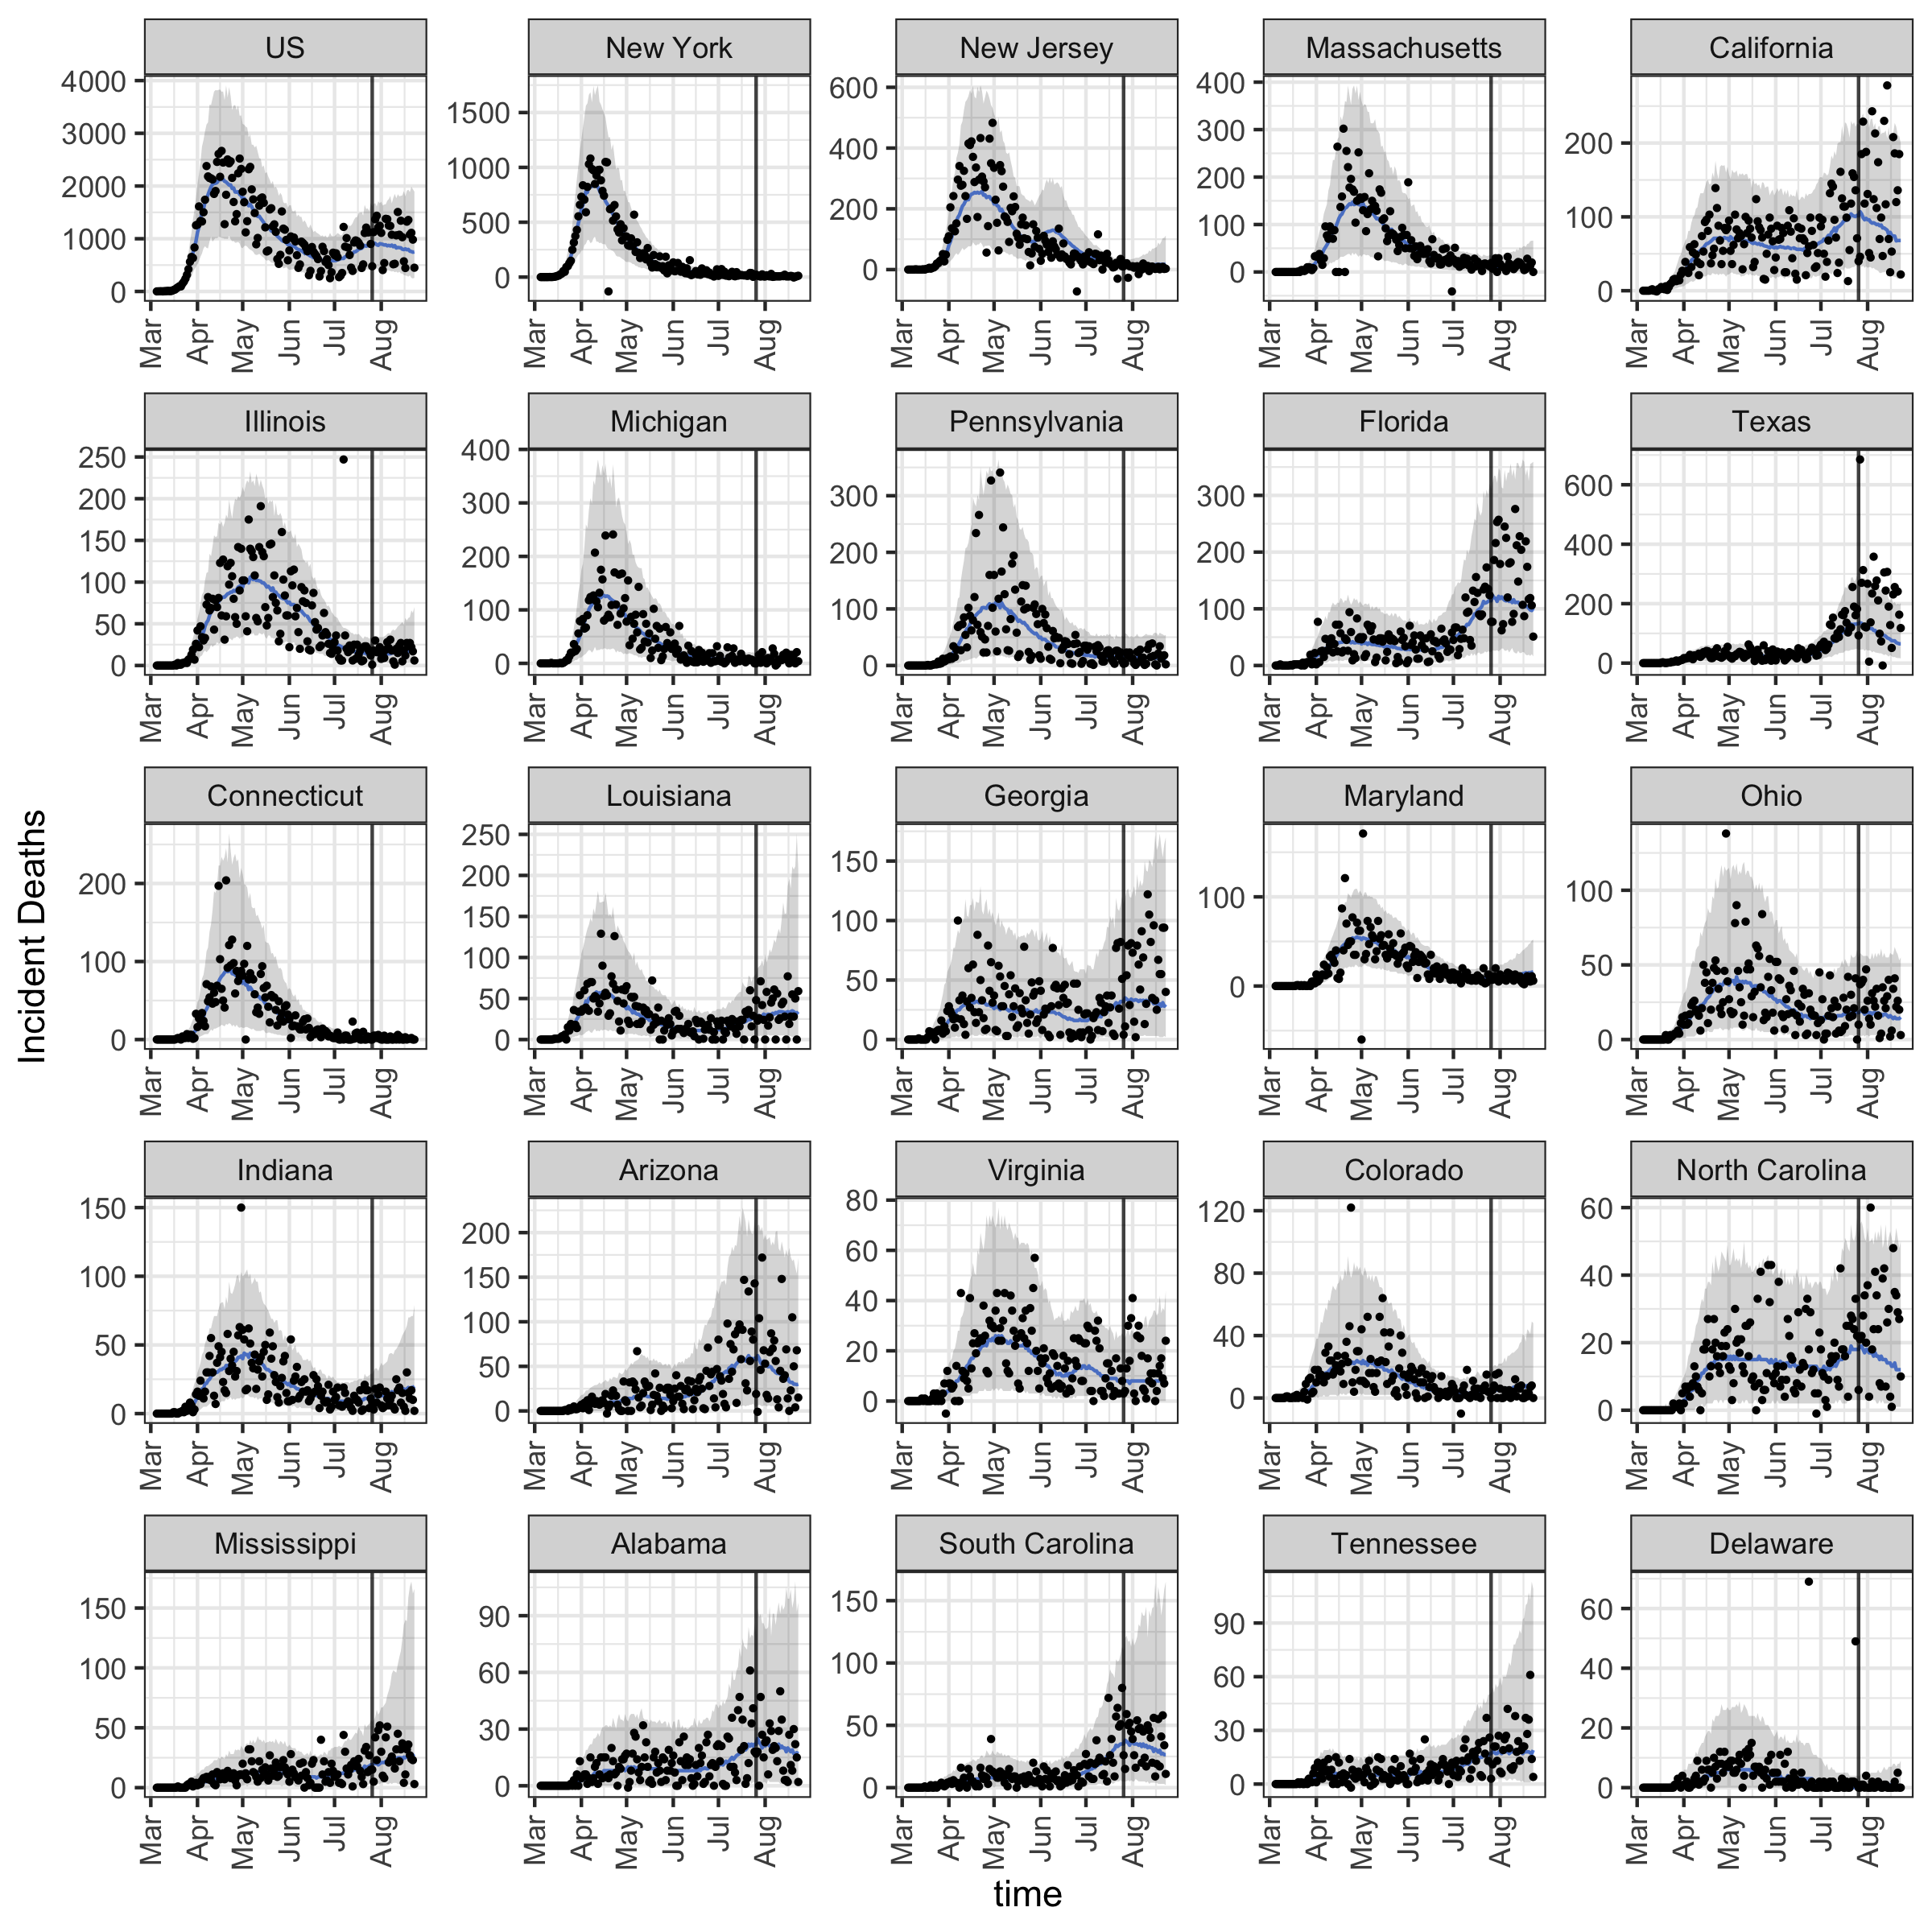
\includegraphics[scale=.2]{fit_and_forecast_results.png}

\caption{Example fit and forecast for 2020-07-26 for states with over 50 incident deaths and the U.S.. Grey bands represent 95\% prediction intervals. Blue line represents median forecast. MechBayes is able to produce well calibrated fits to the data as well as accurately tracking trends in incident deaths.}
\label{fig:fit_and_forecast_results}
\end{figure}

	
 
\begin{figure}
  \centering
     \begin{subfigure}{1\textwidth}
  \centering
    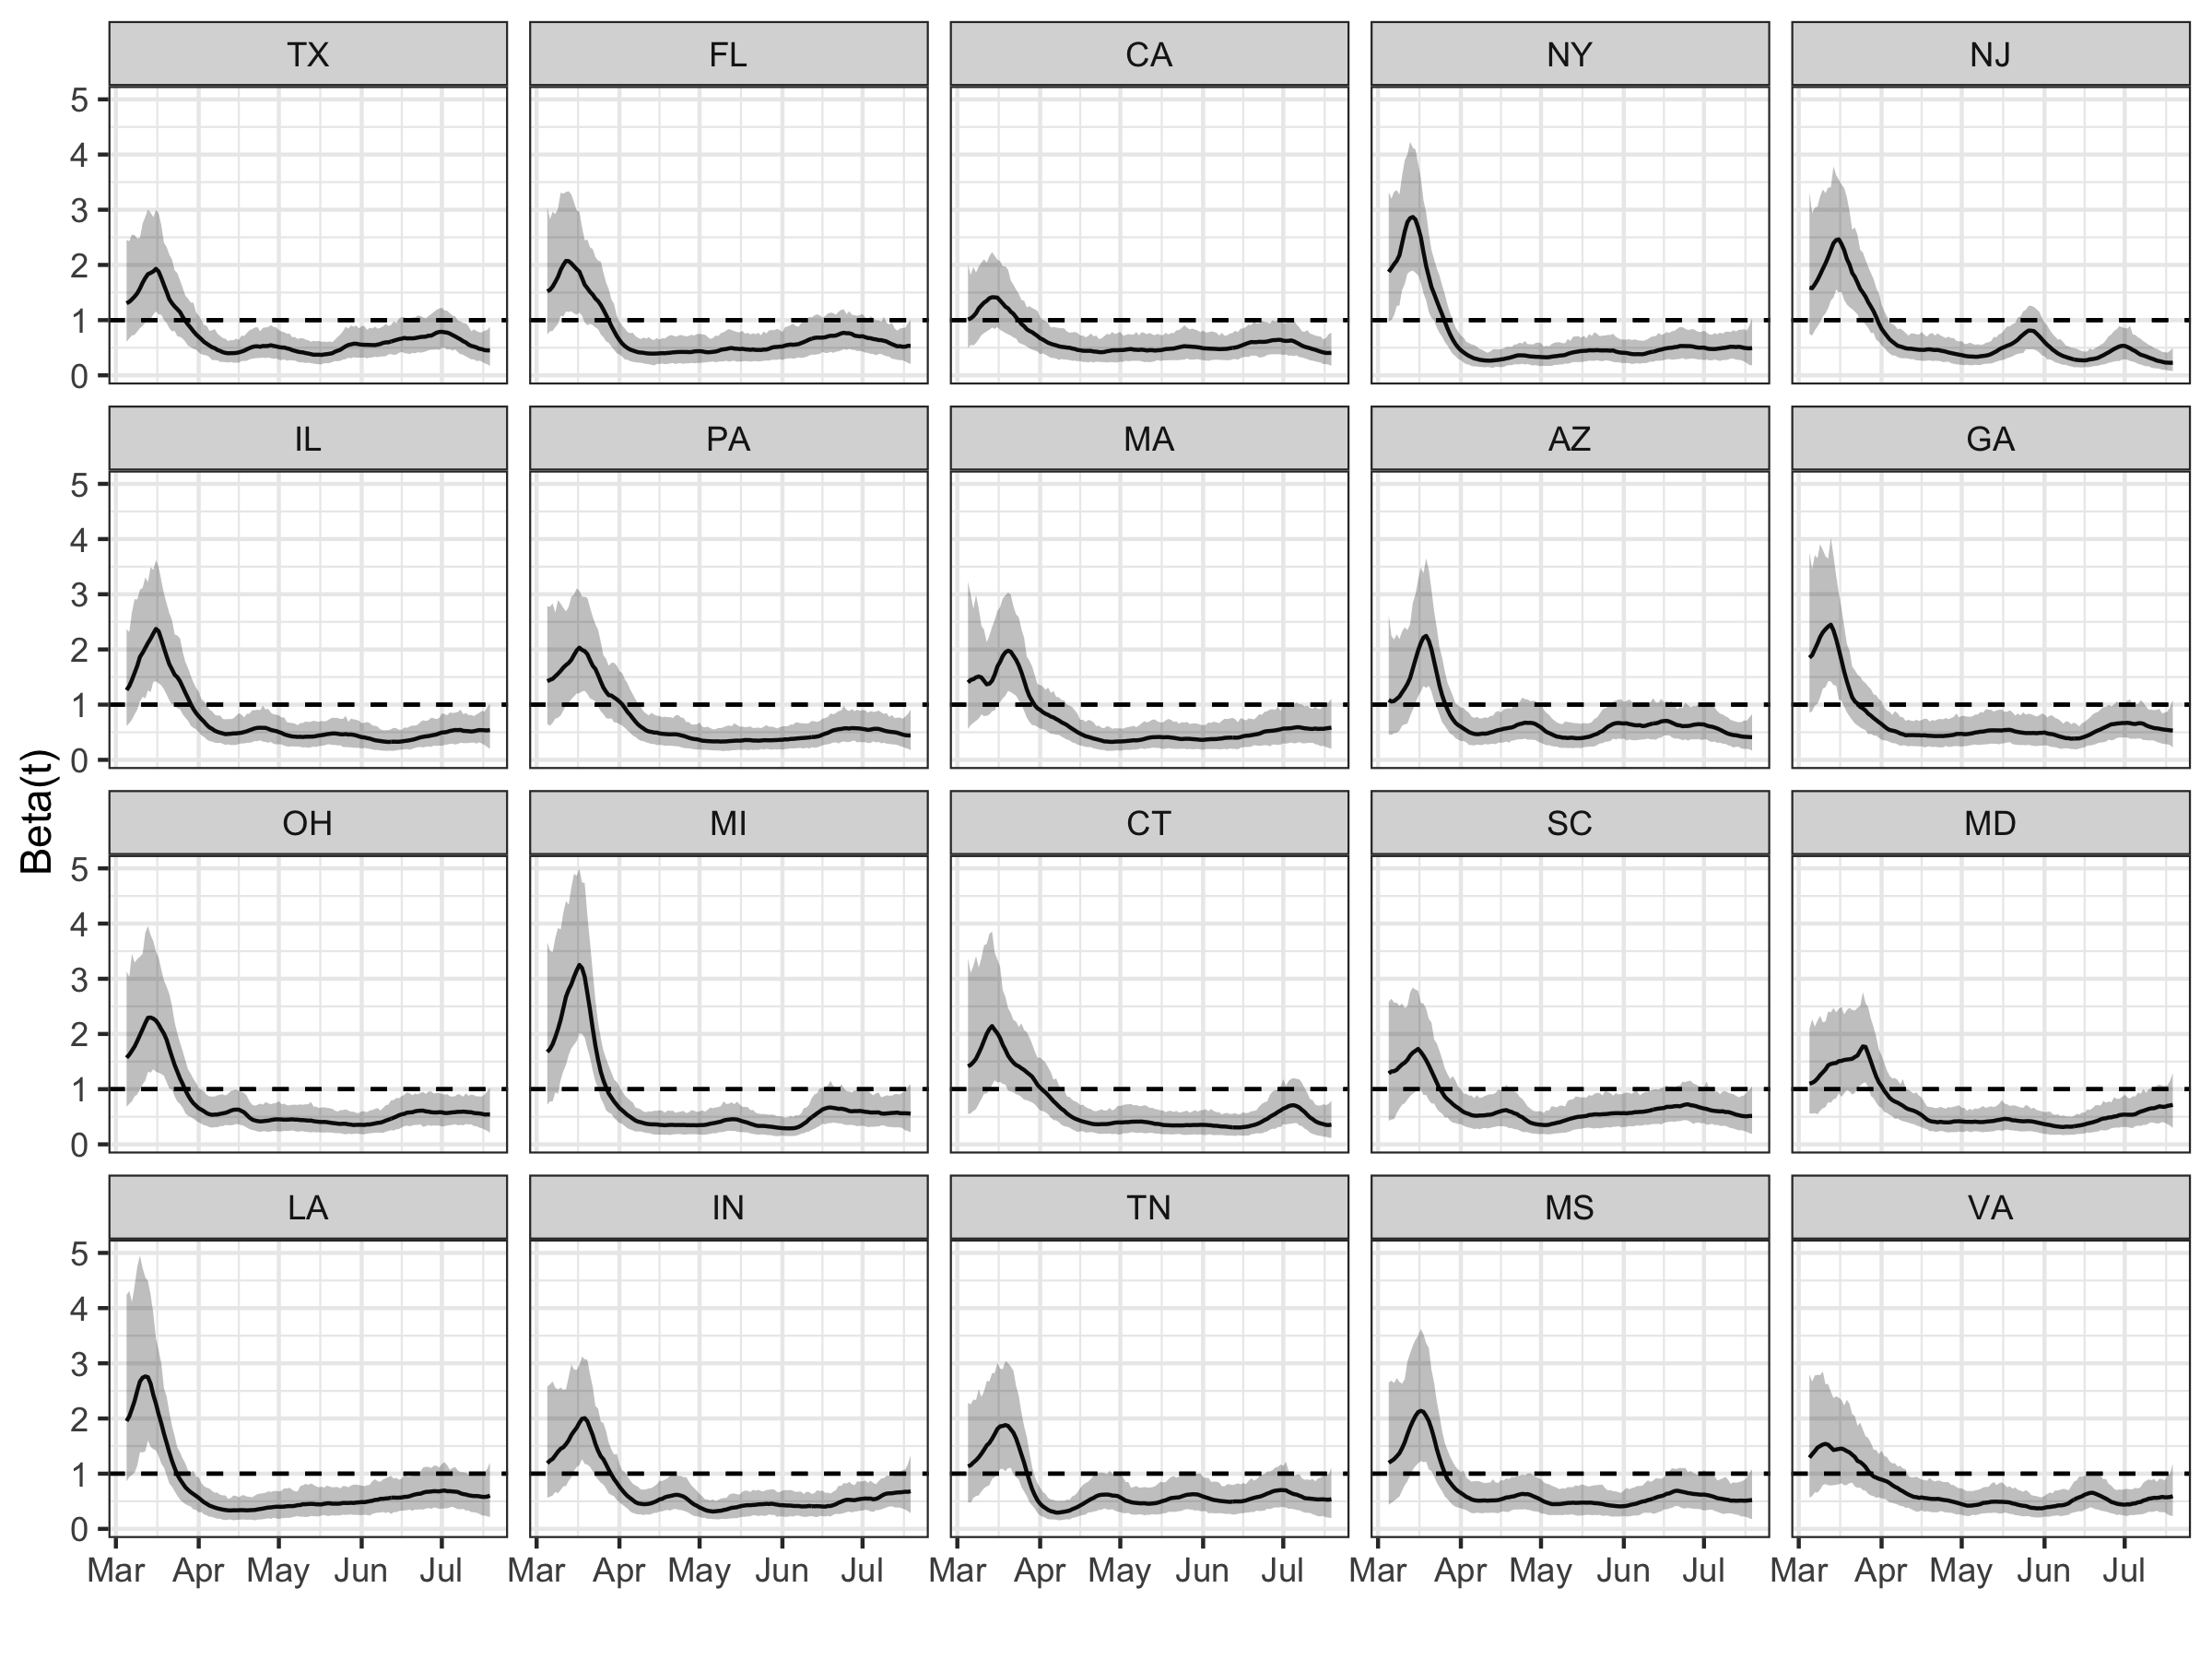
\includegraphics[scale=.15]{beta_t_plot.png}
    \caption{Time-varying beta ($\beta(t)$).}
\end{subfigure}

\begin{subfigure}{1\textwidth}
  \centering
    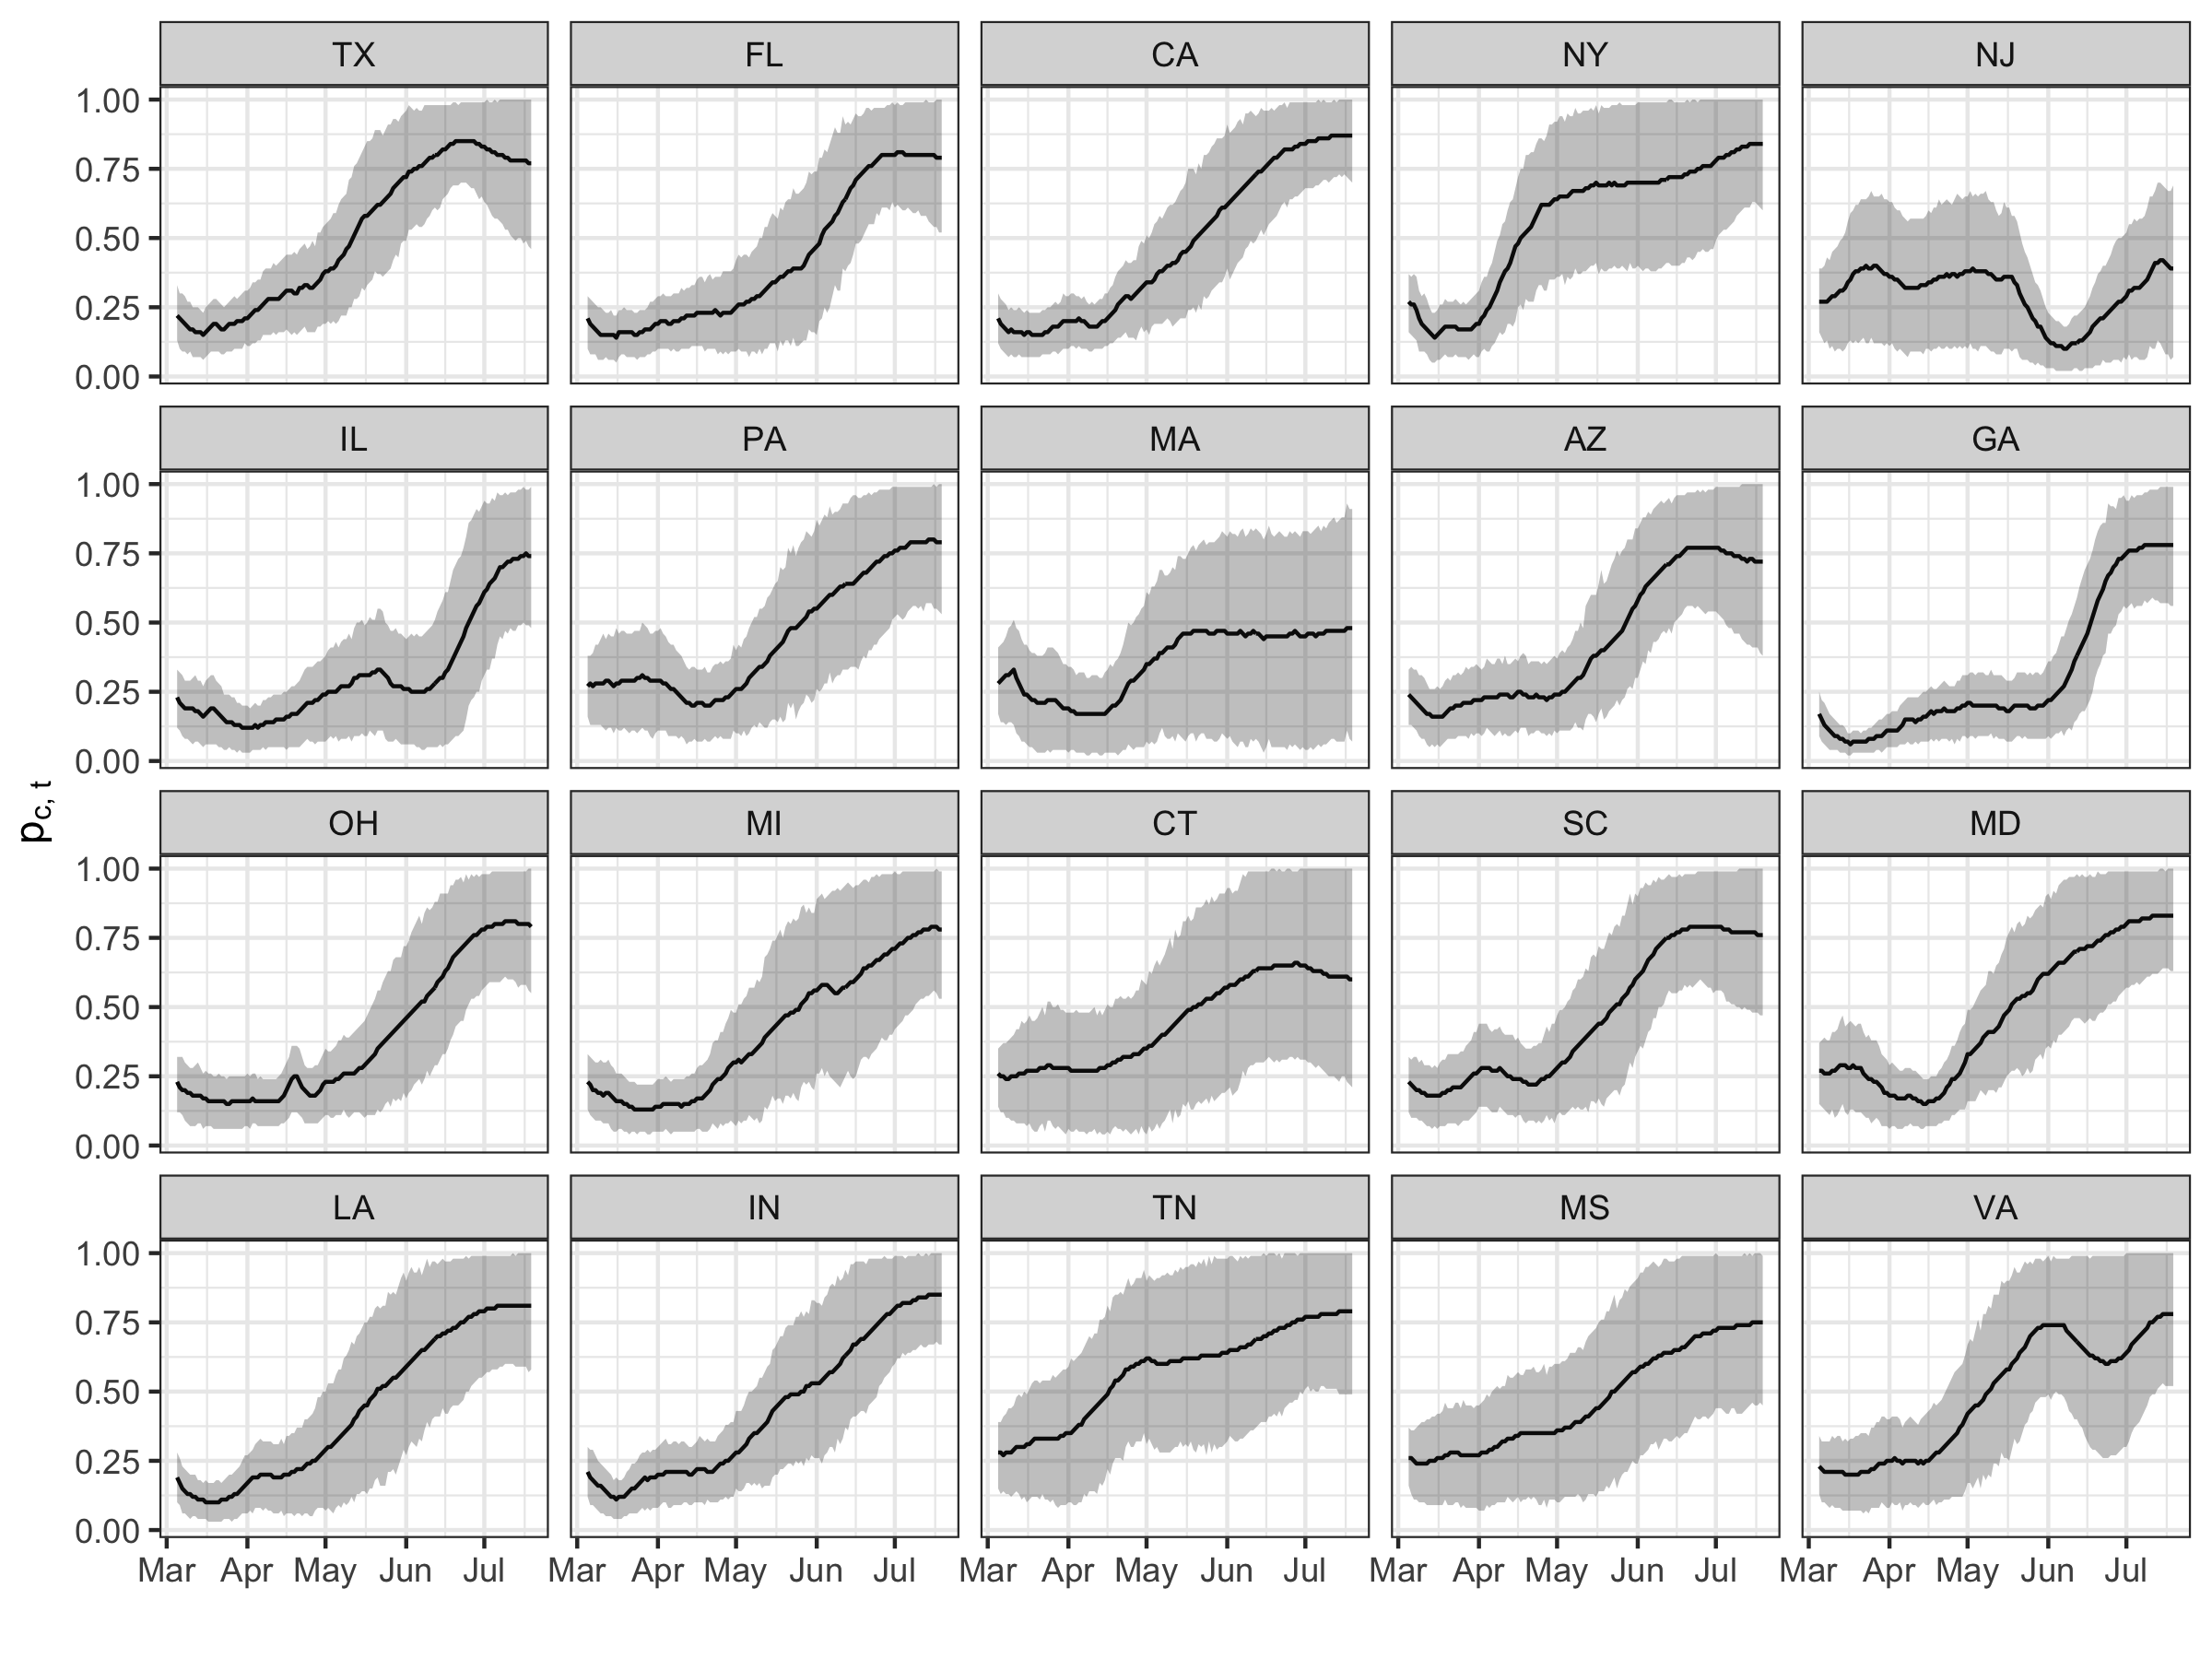
\includegraphics[scale=.15]{detection_plot.png}
    \caption{Time-varying case and death deviation model ($p_{c,t}$)}
\end{subfigure} 
 \caption{  A) Time varying beta parameter for all states with a day exceeding 50 incident deaths, including the U.S. by 2020-07-26. We can clearly see that the random walk is able to account for a composite of intervention efforts. B) Time varying case and death deviation model for example states. The time varying case and death deviation model is able account for the increase in testing and other reporting anomolies.}
\label{fig:model_details}
\end{figure}

\section{Real-time Forecasting Results}

We can see from Figure \ref{fig:fit_and_forecast_results} that MechBayes is able to accurately model the observed data. The model is able to adapt to highly variable incident death reporting, variable transmission rates, and overall heterogeneity of incidence curves. The model is also able capture the uncertainty of the differential equation parameters well enough to produce well calibrated prediction intervals. Figure \ref{fig:fit_and_forecast_results}  shows prediction intervals at the 95\% level, with 92.3\% of observations falling within the bounds for each state. However, we can also see that in some states, such as California and Florida, the model is biased high, with all observations outside of the 95\% prediction interval falling below. Figure \ref{fig:fit_and_forecast_results}  also shows 4 weeks of daily forecasts, along with the daily observed incidence for 1 week out. We can see that the predictions are tracking the data even under the weekly reporting cycles. 

We can see from Figure \ref{fig:model_details} that MechBayes is able to learn to adapt to the evolving pandemic situation. Panel A shows the time-varying transmission $\beta(t)$ for 20 states with the highest total deaths. We can see that $\beta(0)$ is centered on our prior but as data comes in, the estimate increases. This is especially true in NY, where the epidemic took off quickly in March. However, the model is then able to adjust to the varying levels of interventions present in each state. This radically reduces the transmissibility parameter by the first week of April 2020 for almost all states. This is consistent with a peak in overall deaths two weeks later in mid-April 2020. There seems to be some estimation issues at the boundary of $\beta(t)$ where the number of cases does not match the number of deaths, since the cases have not yet converted to deaths. This results in the model underestimating transmissibility to reduce the flow through the compartments. 

We can also see from Figure \ref{fig:model_details}  that MechBayes is able to account for the drastic increase in testing that has occurred across the U.S. since March 2020. Panel B also shows that our prior estimate of 30\% of cases being detected, may have been too high, as all regions show a dip in case and death deviation model before climbing again. 

%Note that interpreting this strictly as time-varying detection is obscuring the fact that this parameter $p_{t,d}$ can soak-up any excess variation beyond the ability of cases and the case-fatility ratio to explain the number of deaths. That is, the time-varying case and death deviation model is able to "de-couple" cases and deaths beyond the case-fataility ratio regardless of the underlying reason (whether that be an increase in testing or shifting age distribution of cases). Thus, interpretation of this parameter as a strict mapping to testing is incorrect. As a forecasting model, we only need the ability to non-parametrically model deviations and reporting issues in cases.



\begin{figure}
  \centering
     \begin{subfigure}{.5\textwidth}
  \centering
    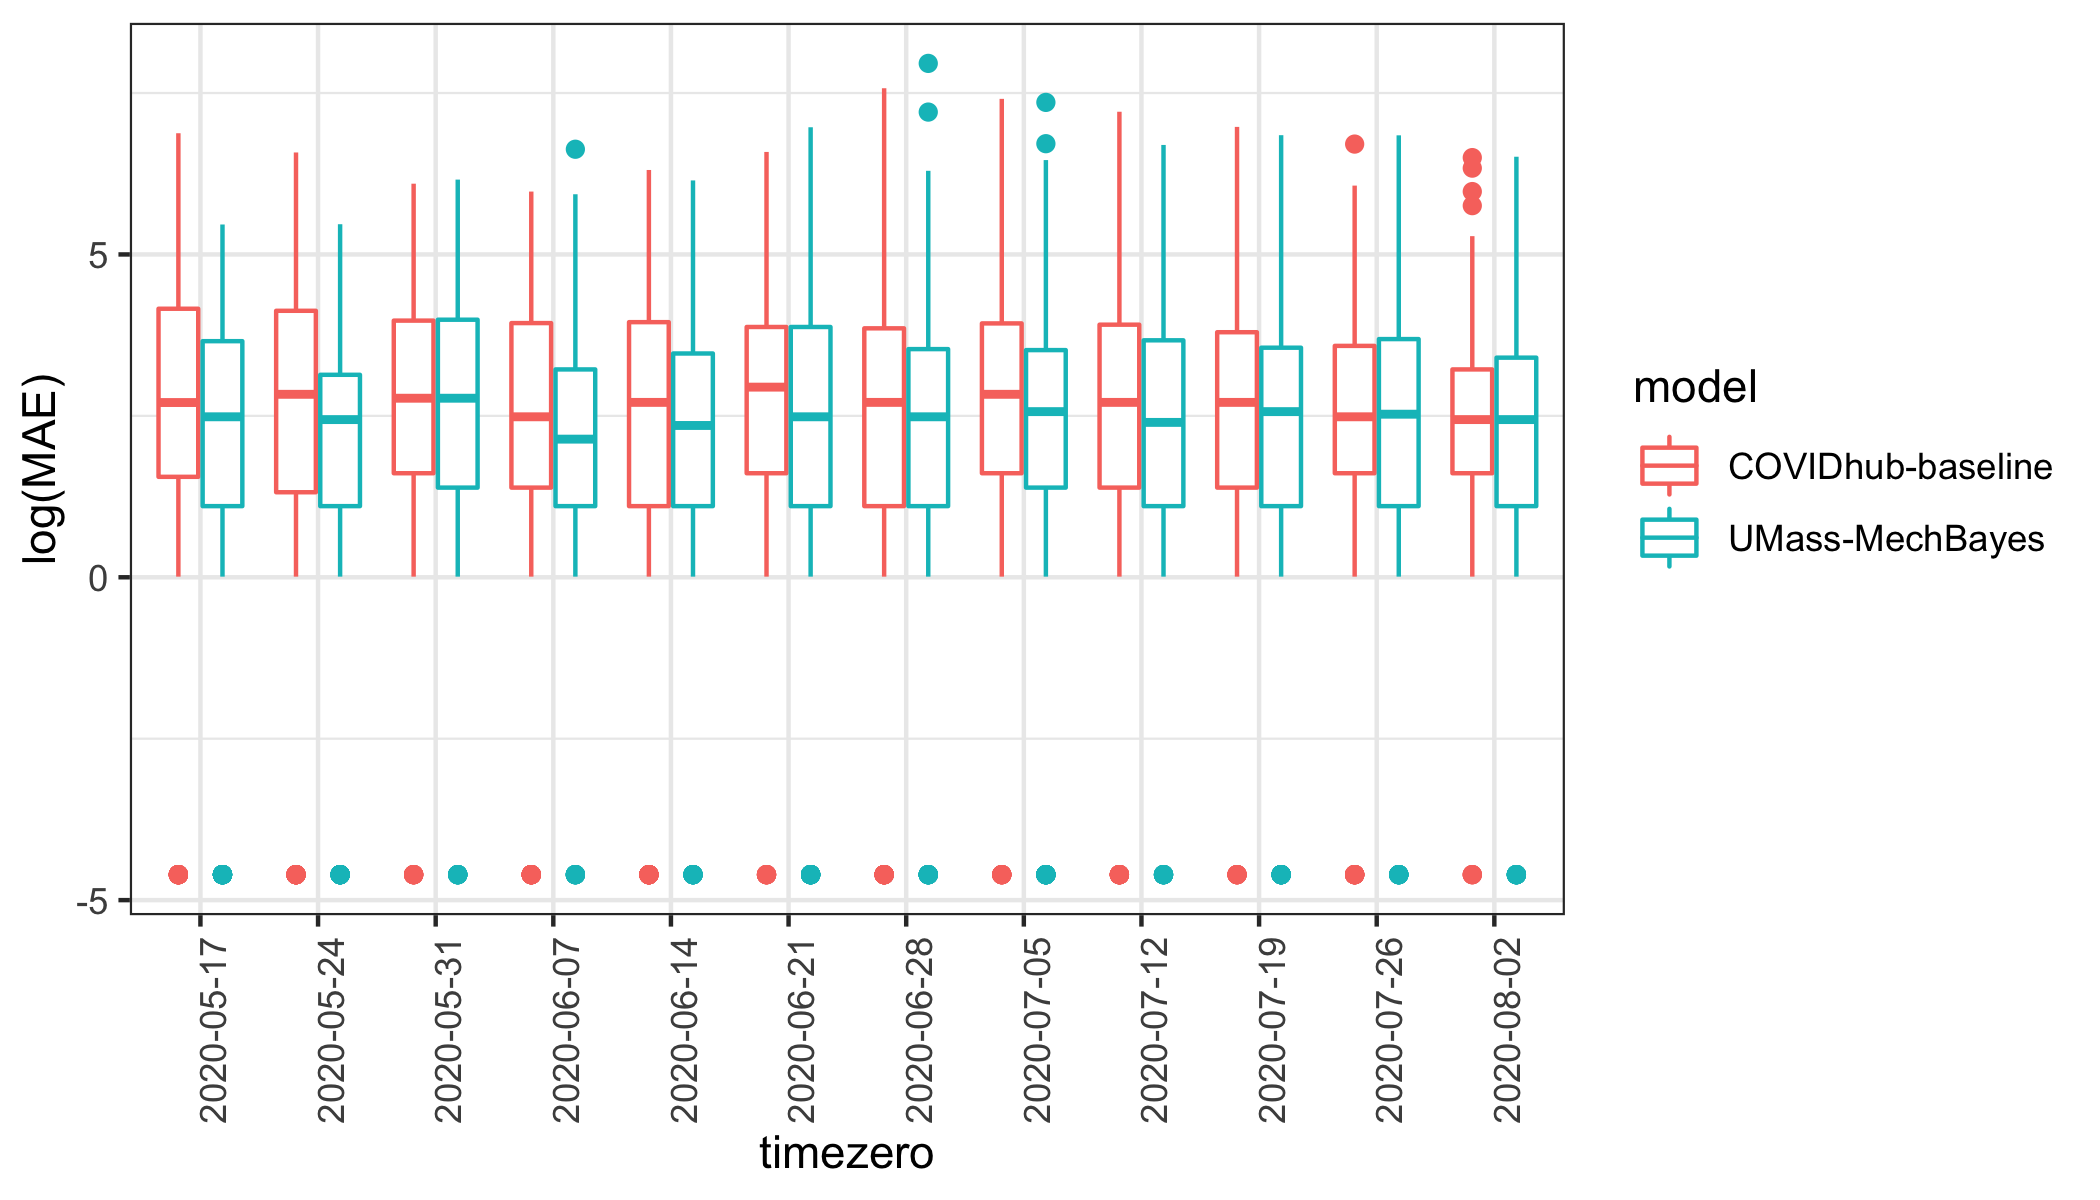
\includegraphics[scale=.135]{mae_results_by_time_zero_inc.png}
    \caption{MAE by forecast week}
\end{subfigure}%
\begin{subfigure}{.5\textwidth}
  \centering
    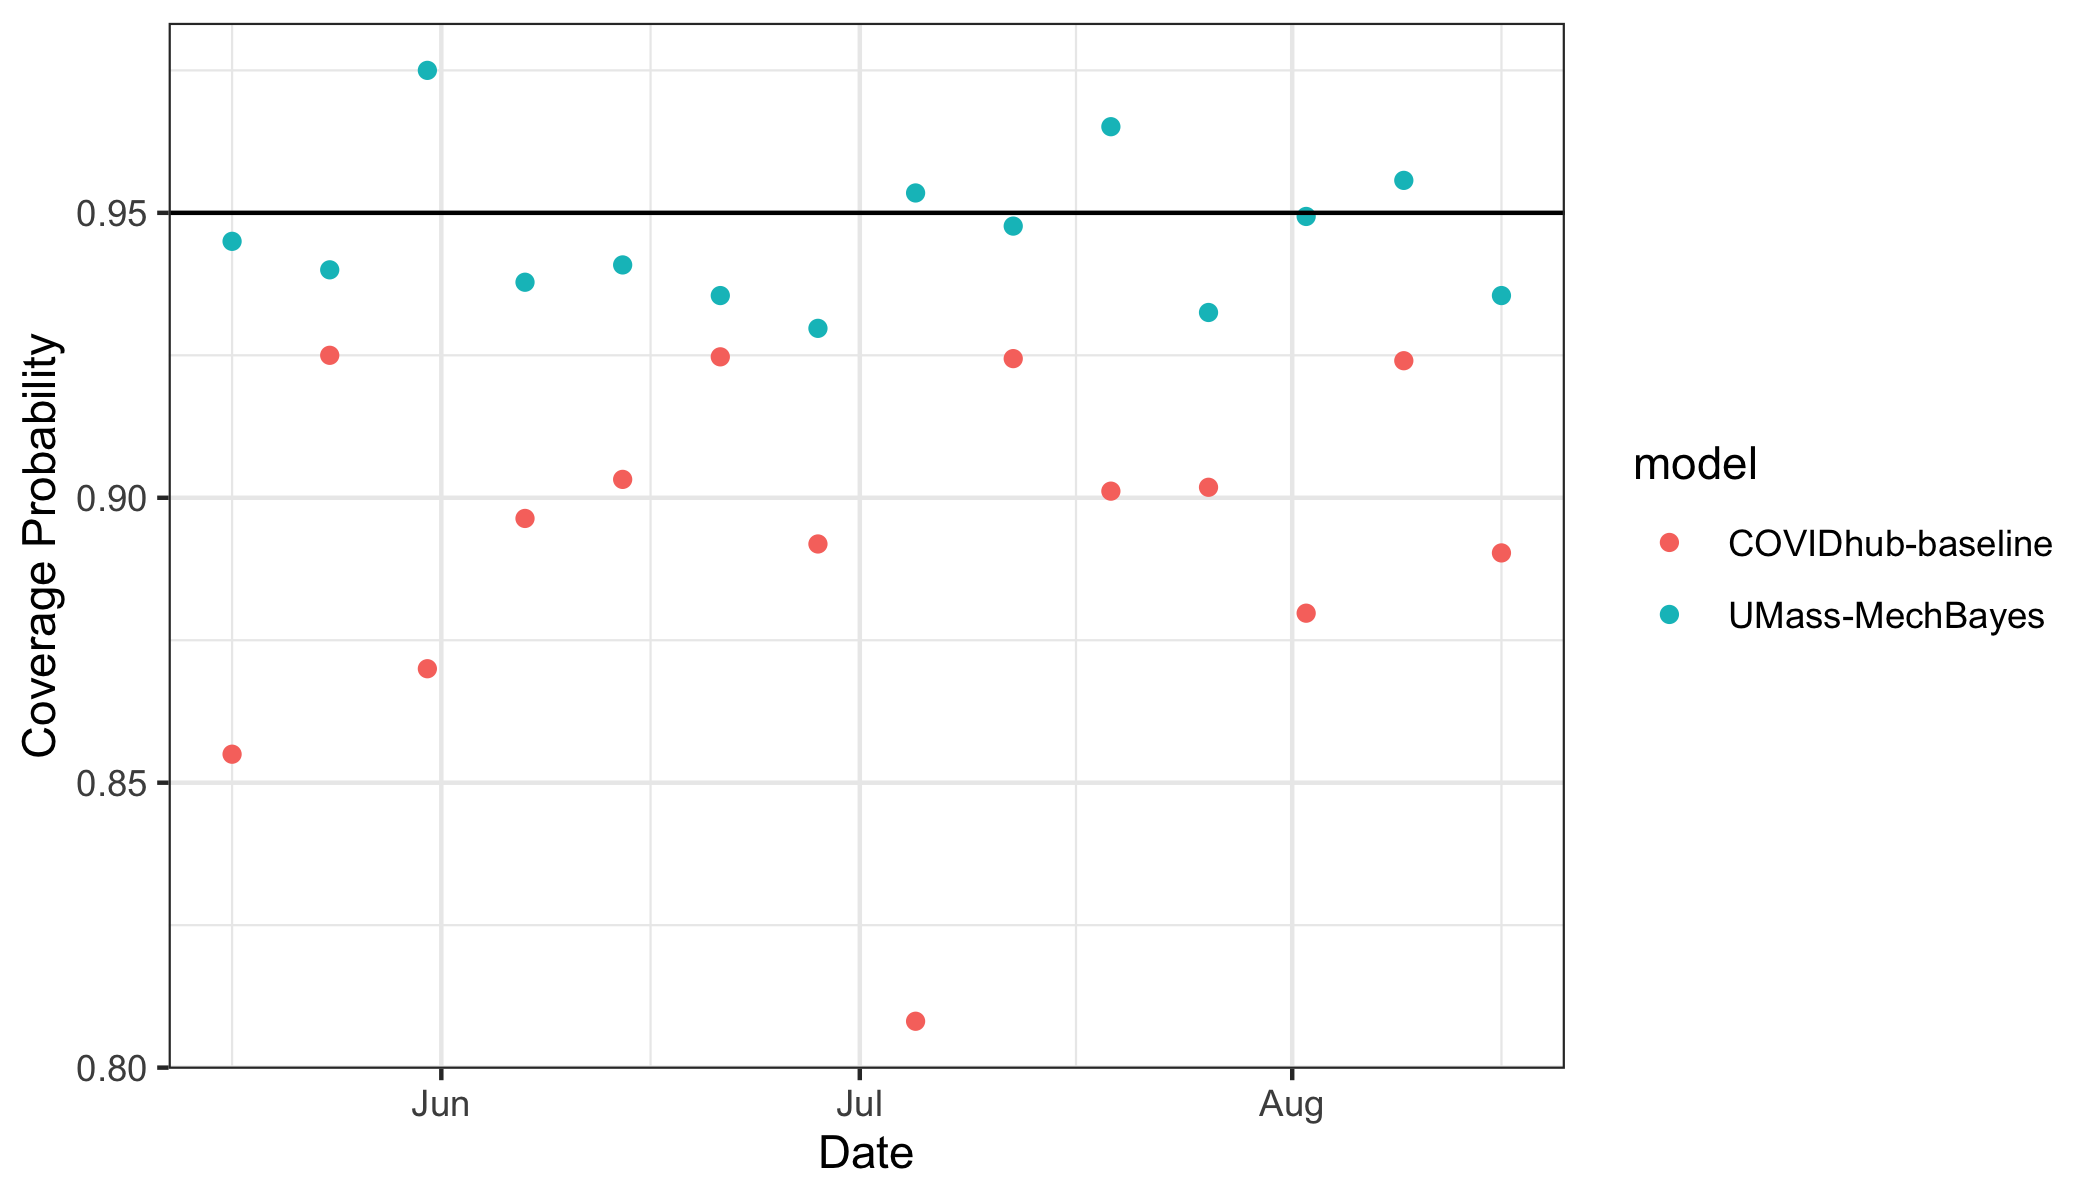
\includegraphics[scale=.115]{cp_results_by_time_zero.png}
    \caption{Coverage probability by forecast week}
\end{subfigure}
\begin{subfigure}{.5\textwidth}
  \centering
    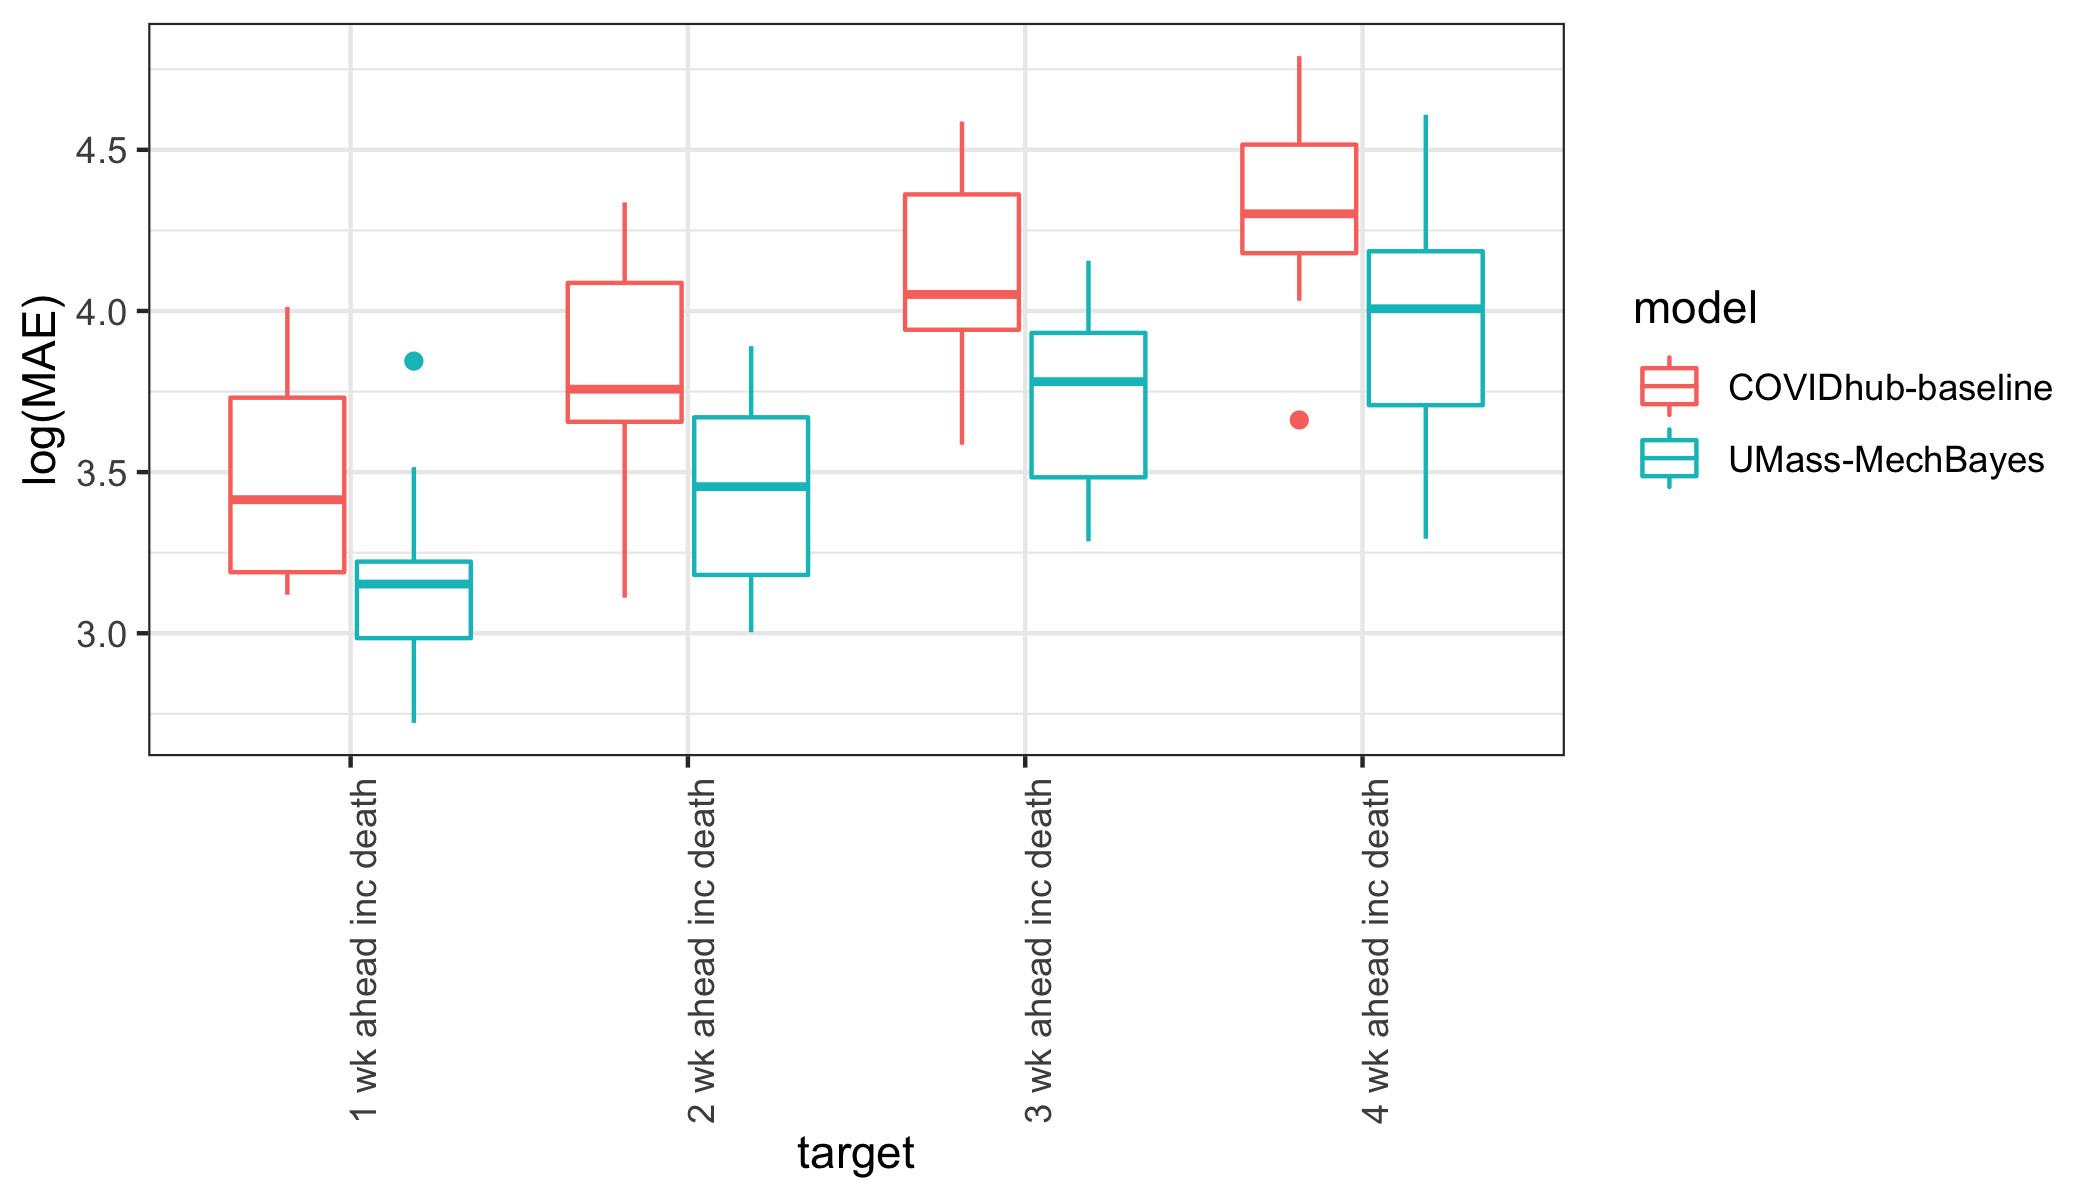
\includegraphics[scale=.135]{mae_results_by_target_inc.png}
    \caption{MAE by target}
\end{subfigure}%
\begin{subfigure}{.5\textwidth}
  \centering
    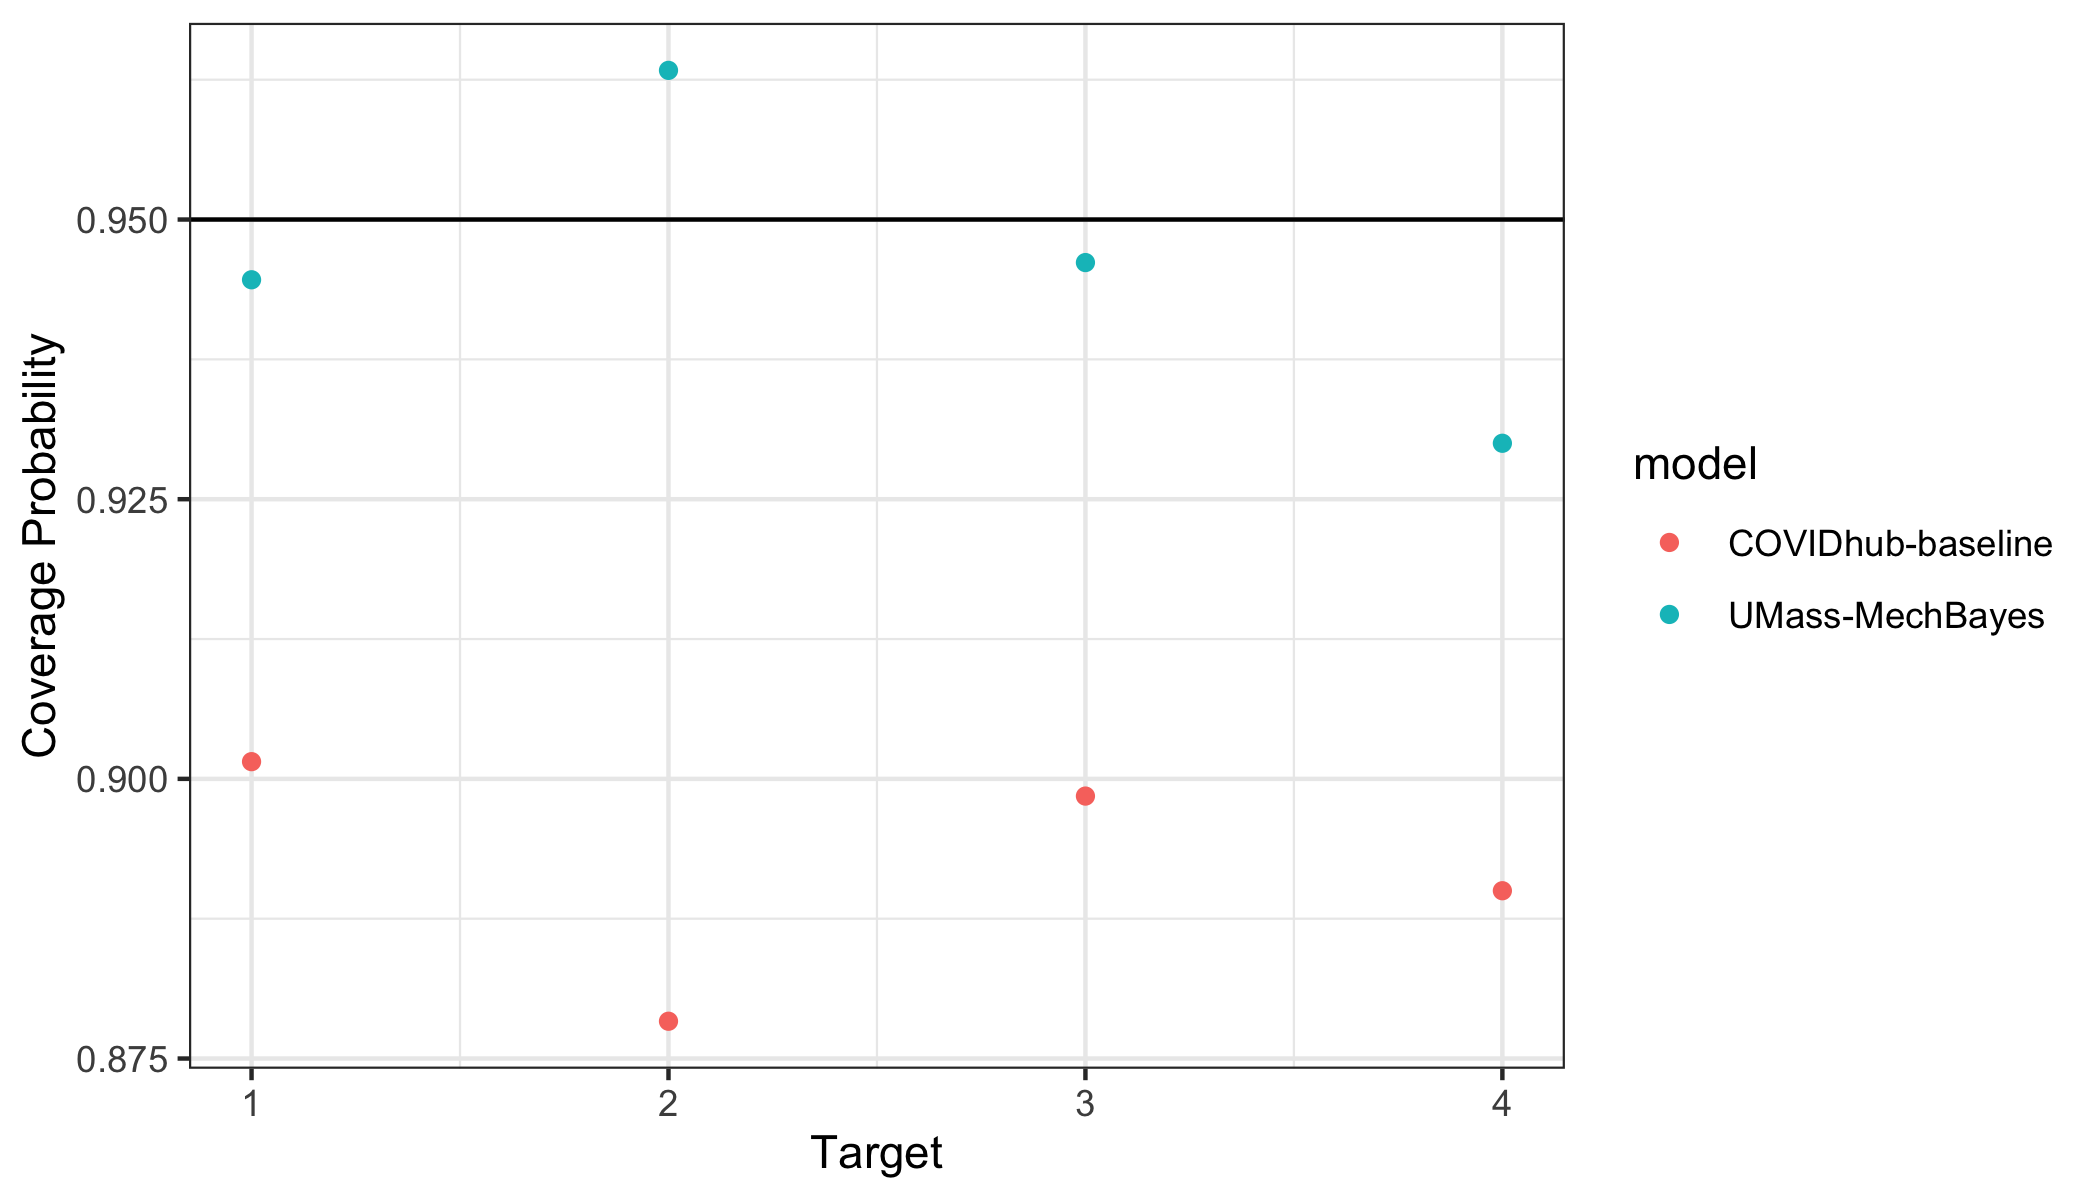
\includegraphics[scale=.115]{cp_results_by_target.png}
    \caption{Coverage probability by target}
\end{subfigure}%

\caption{Scores from COVID-19 Forecast Hub broken down by target and forecast week. MechBayes improves in average MAE in 9 out of 12 timepoints. MechBayes improves in MAE across all targets. We can see that as the horizon increases from 1 to 4 weeks ahead, MAE, reflecting an increase in difficulty of forecasting further ahead in time. We also see a uniform improvement in coverage probability when broken down by timezero and target. Here the horizontal line represents 95\% coverage interval. }
\label{fig:covidhub}
\end{figure}


\begin{figure}
  \centering

\begin{subfigure}{\textwidth}
  \centering
    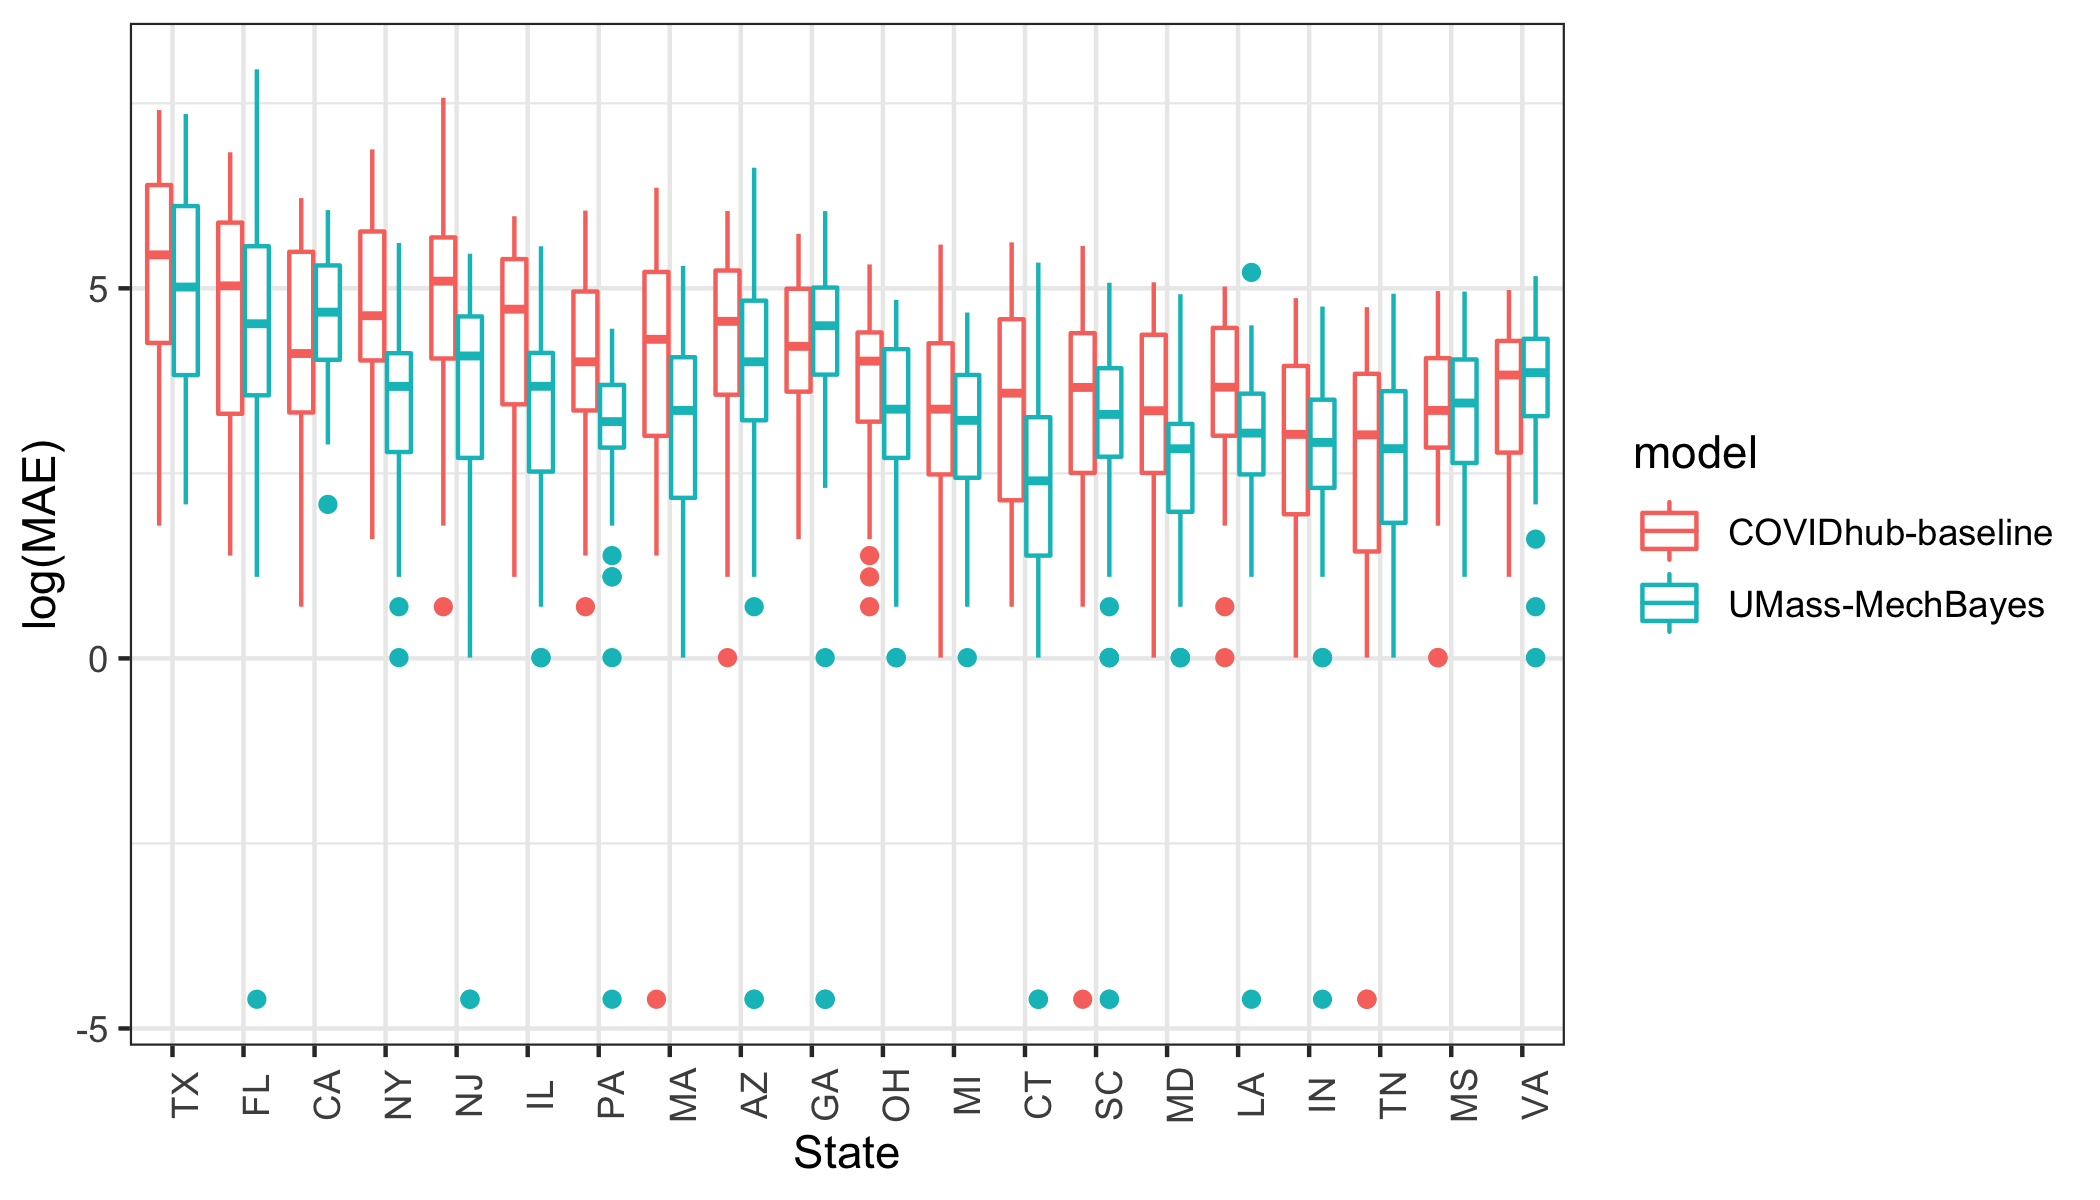
\includegraphics[scale=.2]{mae_results_by_region_inc.png}
    \caption{MAE by region}
\end{subfigure}
\begin{subfigure}{\textwidth}
  \centering
    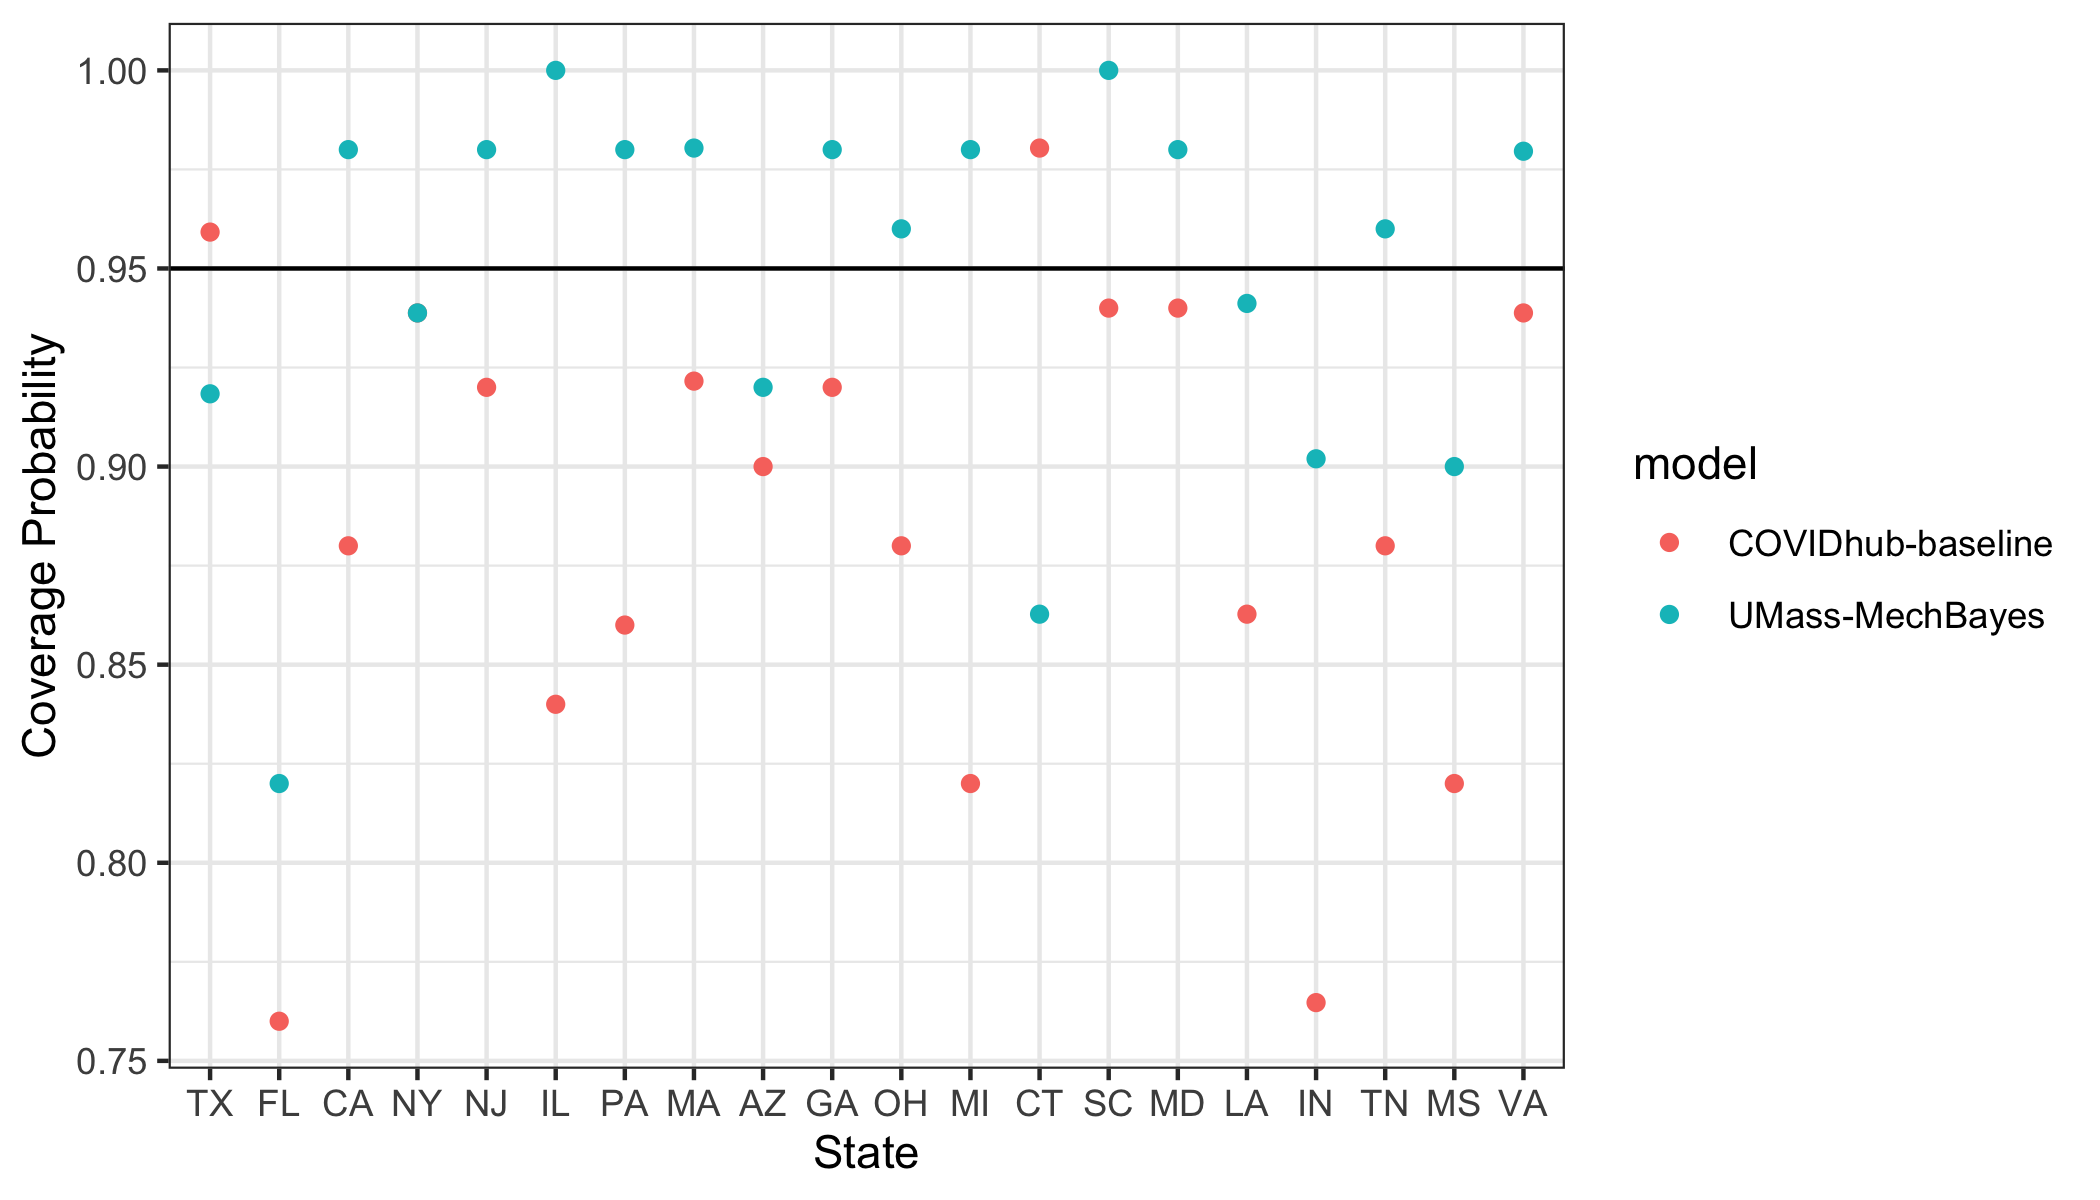
\includegraphics[scale=.20]{cp_results_by_location.png}
    \caption{Coverage probability by region}
\end{subfigure}
\caption{Scores from COVID-19 Forecast Hub broken down by region for the 20 regions with the highest incident deaths. Regions are sorted by total deaths left to right. Here we can see that MechBayes has the greatest increase in states with large total death counts. States with medium or small death counts have more mixed results. The improvements in coverage probability are more mixed, with MechBayes improving coverage probability in 12 of 20 regions. }
\label{fig:covidhub_region_results}
\end{figure}


\section{Real-Time Model Results}

We next turn to the comparison of MechBayes against the COVID-19 Forecast Hub baseline model. This baseline model uses the previous daily incident as the mean forecast for the current daily incidence, along with  bootstrapped prediction intervals from historical changes in daily incidence. See COVID-19 Forecast Hub for more details. \cite{covidhub}. 

We begin by breaking down the results by week the forecast was made (forecast week) and averaging over both region and target. As we can see from Figure \ref{fig:covidhub} (A,B), MechBayes outperformed the COVID-19 Forecast Hub baseline on MAE and coverage probability when broken down by forecast week. However, the improvements broken down by time are small, and improves in 9 out of 12 evaluation weeks.  As we can see from \ref{fig:data}, in weeks with the largest increase in deaths (mostly during the month of May) MechBayes significantly outperformed the baseline model. However, in weeks with a small increase or a decrease in deaths, the scores were much closer. This suggests that MechBayes performs well where it counts, when the epidemic is taking off nearly exponentially. 

We also break down the results by geographical region, as seen in Figure \ref{fig:covidhub} (C,D). Here we see consistent improvements in MAE under MechBayes for regions with high total death counts with an improvement in the average MAE in 16 out of the 20 states with the highest total death count. Out of the states with the 10 highest death counts, only in California did the baseline model outperform MechBayes on the average MAE. However, the results are more mixed for states with lower death counts.

We break down the results by target by averaging over region and forecast week  \ref{fig:covidhub} (E,F) Here we can see uniform improvement over the baseline model by MechBayes in terms of MAE and coverage probability. We can also see that the MAE increase as horizon increase, which is to be expected. We can also see that incident MAE is lower than cumulative MAE, which is again to be expected due to the lower absolute numbers of incident deaths. 

Finally, we include a formal test of the difference in MAE to demonstrate statistically significant advantages in using MechBayes over the baseline model. In order to do this, we just a random effects regression model of the form,

\begin{eqnarray*}
log(MAE_{m,t,r,h} +1) &=& \beta_0 +  \beta1*h_1 + ....+ \beta_3*h_3 \\
&+& \beta_4 *h_1*mb + .... \beta_8*h_4*mb\\
 &+& b_{r} + \epsilon \\
b_{r} &\sim &N(0,\Sigma_b^2)\\
\epsilon &\sim& N(0,\sigma^2)
\end{eqnarray*}

where $mb$ is an indicator for the MechBayes model, $t$ is timezero, $r$ is region, and $h$ is target horizon (1-4 week ahead). We chose this model because it explains the variation in MAE by model and horizon while allowing varying baseline MAE values by region. Here, variation over time in MAE within a specific region is explained by differences in model performance This leads to the following coefficient estimates for the fixed effects.

\begin{table}[ht]
\centering
\begin{tabular}{rrrrrr}
  \hline
 & Estimate & Std. Error & df & t value & Pr($>$$|$t$|$) \\ 
  \hline
$\beta_0$  & 2.47 & 0.17 & 54.87 & 14.97 & 0.00 \\ 
   $\beta_{h_1}$ & 0.30 & 0.06 & 4643.00 & 5.18 & 0.00 \\ 
 $\beta_{h_2} $ & 0.44 & 0.06 & 4643.00 & 7.56 & 0.00 \\ 
  $\beta_{h_3}$ & 0.59 & 0.06 & 4643.00 & 9.79 & 0.00 \\ 
  $\beta_{h_1 mb}$  & -0.19 & 0.06 & 4643.00 & -3.19 & 0.00 \\ 
  $\beta_{h_2 mb}$ & -0.29 & 0.06 & 4643.00 & -4.87 & 0.00 \\ 
   $\beta_{h_3mb}$ & -0.23 & 0.06 & 4643.00 & -3.94 & 0.00 \\ 
 $\beta_{h_4mb}$ & -0.29 & 0.06 & 4643.00 & -4.72 & 0.00 \\ 
   \hline
\end{tabular}
\caption{Coefficient estimates and t-values for MAE evaluation model. We can see that MechBayes performs statistically significantly better than the baseline model for 1-4 weeks ahead. The performance increase seems to grow as horizon increases.}
\end{table}

We can see that MechBayes is significantly better for 1-4 weeks ahead. The difference in skill seems to improve as the forecast horizon increases. The model estimates $\beta_{h_4mb}$ = -0.29, which translates to a multiplicative difference of $e^{-.29}=.75$ on the MAE scale. For example, if the basline model MAE for a particular 4 step ahead forecast is 30, one would expect the MechBayes forecast to have an MAE of 22.5.  We demonstrate that the mixed model proposed above fits the MAE results reasonably in Appendix 2.


   \section{Ablation Test Results}

We can see from Figure \ref{fig:ablation} that MechBayes Full is consistently better than MechBayes Death Only or MechBayes Fixed case and death deviation model. The only exception seems to be June 22nd 2020 for the two week ahead target. Late June 2020 is when many states in the U.S. began to see an uptick in cases again, with Texas, Florida, and California seeing their largest total case counts since the beginning of the pandemic. Since MechBayes is conditional on the current level of interventions, forecasts made from June 22nd assumed the same level of intervention present on June 22nd. During this time, each state was re-opening various establishments, while cases were rising. MechBayes Full forecasted an exponential growth in cases, which was reflected in a large over prediction two weeks later on July 4th. Finally, we can also see that the difference in MAE between MechBayes Full and the competing models increases as forecast horizon increases. This suggest that MechBayes Full is a better long term forecasting model.

We can also see that the MechBayes Death Only is consistently better than MechBayes Fixed case and death deviation model.  This may be evidence that naively including case data, without adjusting for discrepancies between cases and deaths due to testing etc., may be worse than not including it at all. 

\begin{figure}
  \centering
     \begin{subfigure}{.5\textwidth}
  \centering
    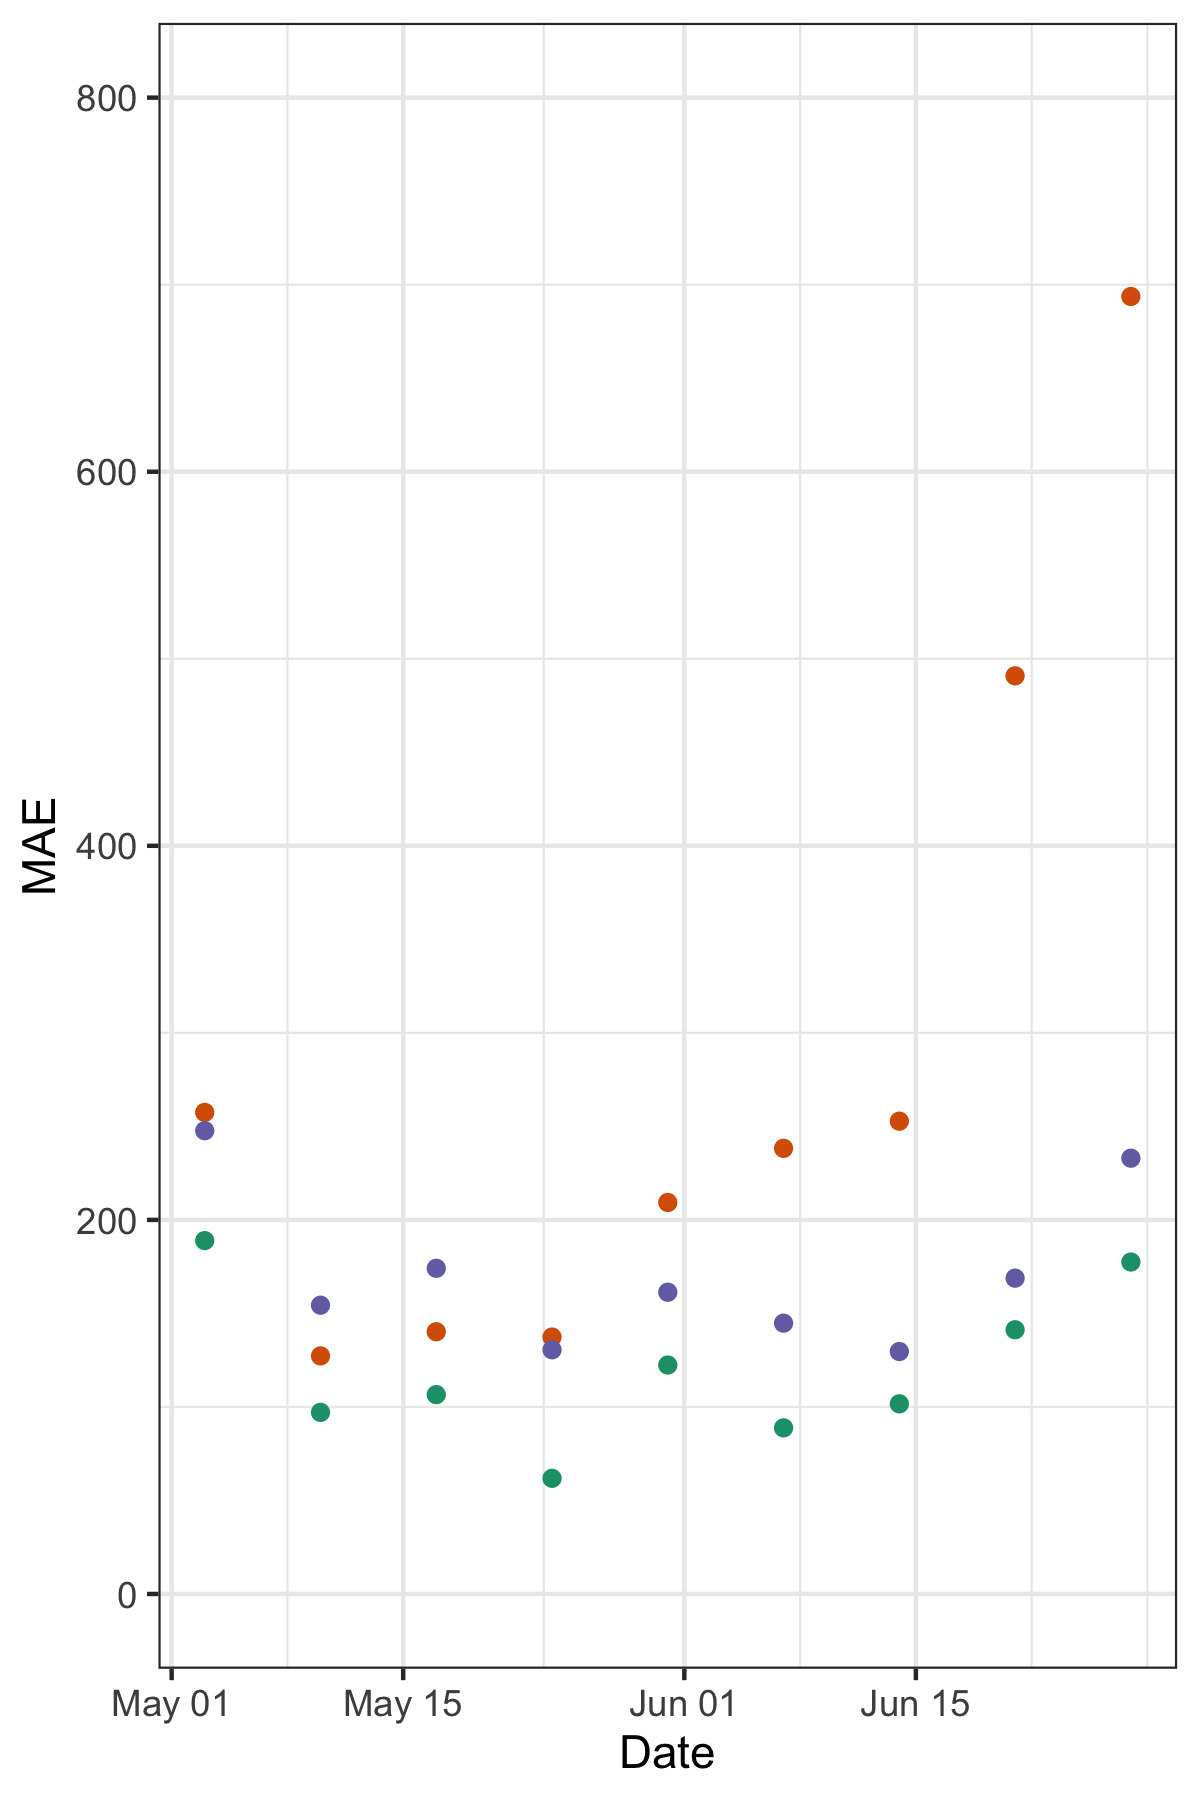
\includegraphics[scale=.15]{ablation_1.png}
    \caption{1 week ahead.}
\end{subfigure}%
\begin{subfigure}{.5\textwidth}
  \centering
    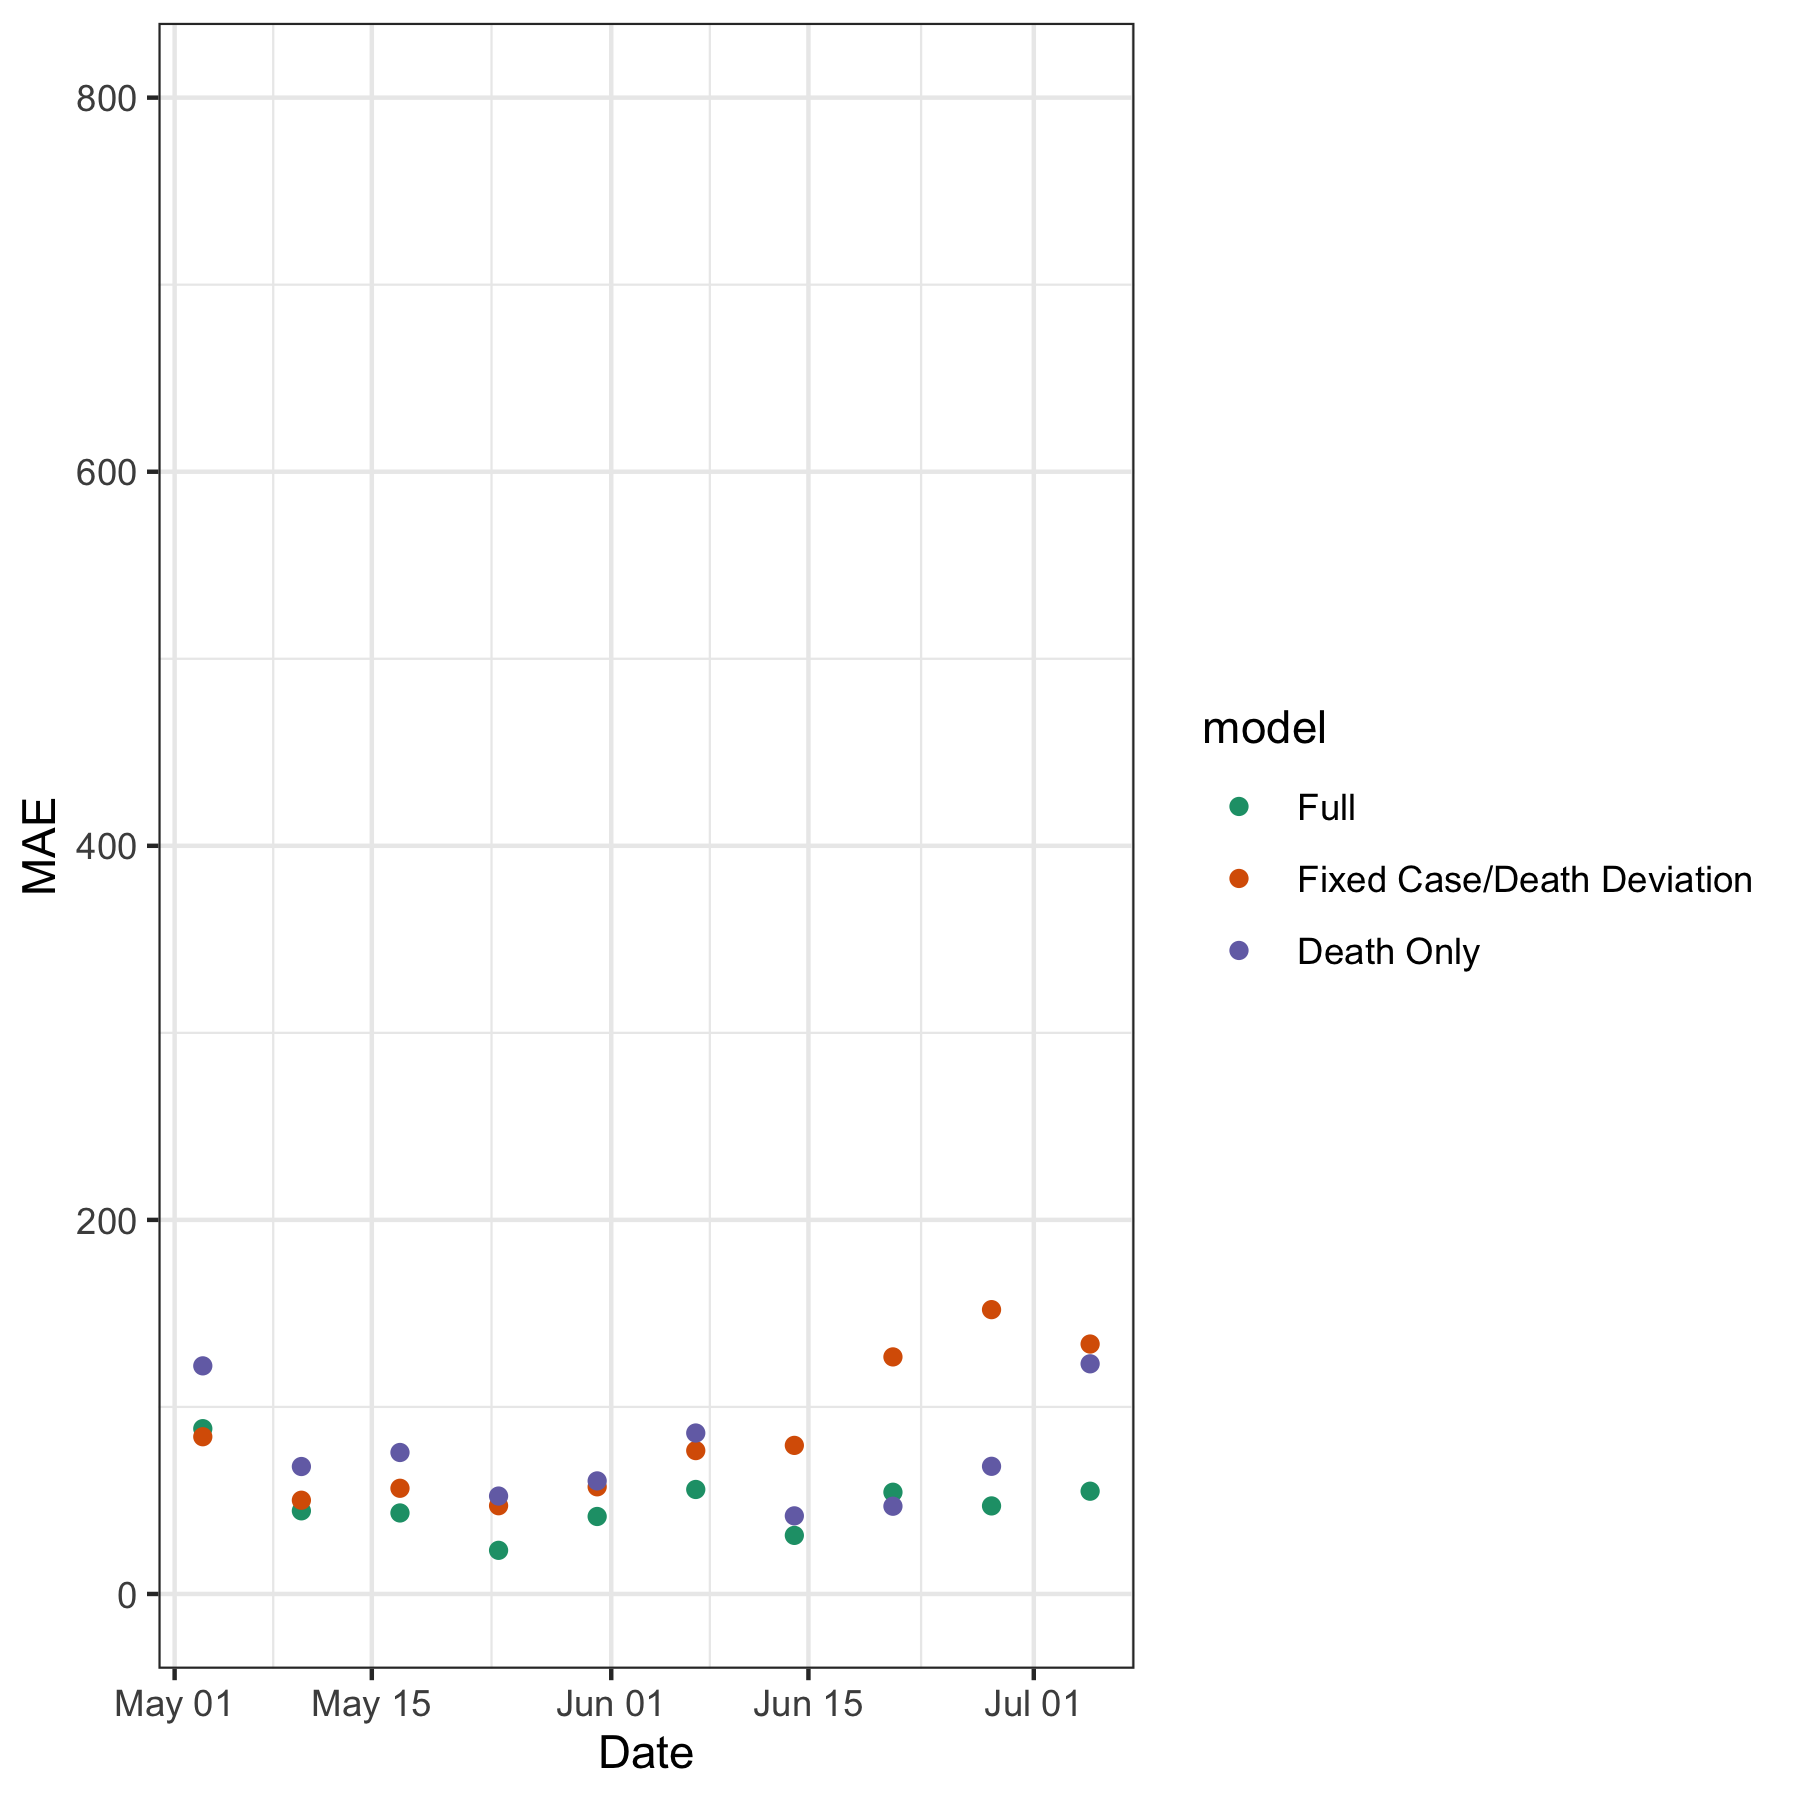
\includegraphics[scale=.15]{ablation_2.png}
    \caption{2 week ahead.}
\end{subfigure}
\begin{subfigure}{.5\textwidth}
  \centering
    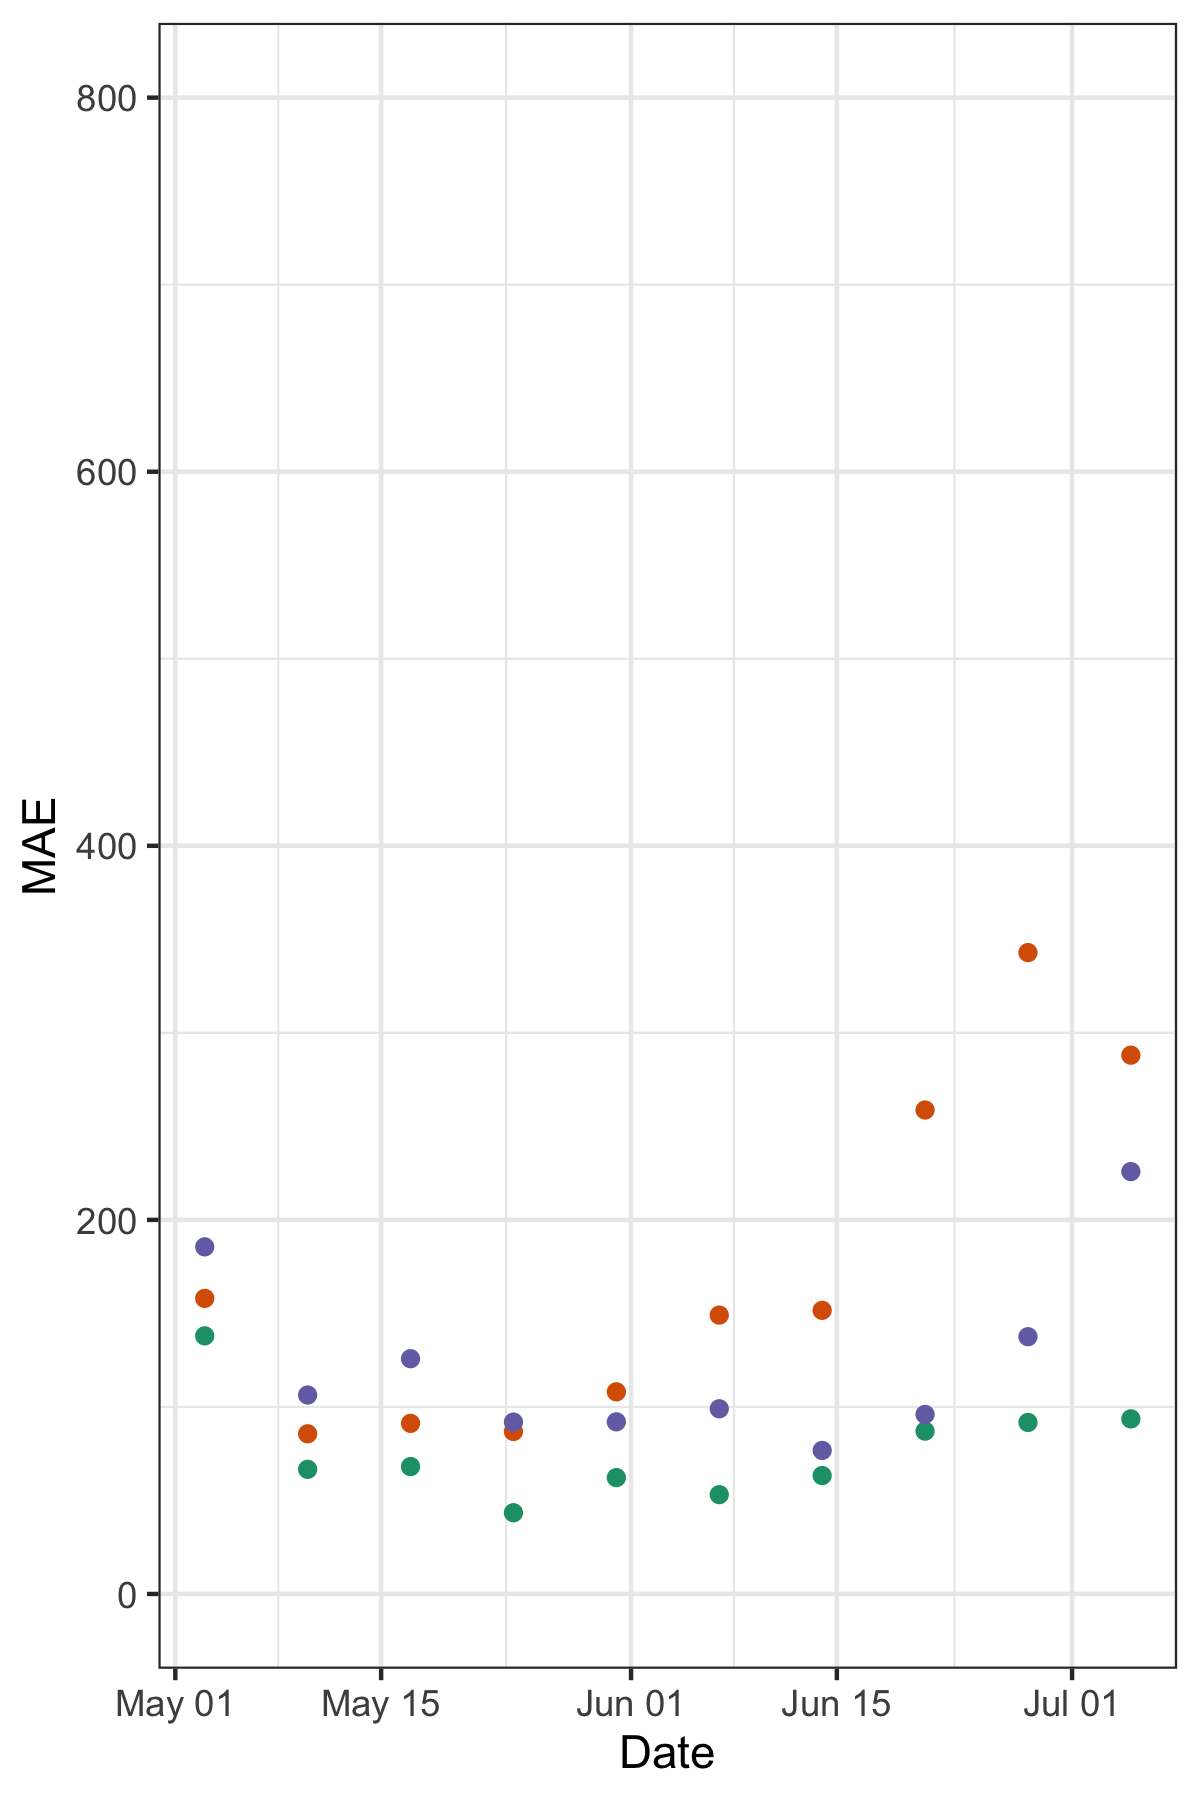
\includegraphics[scale=.15]{ablation_3.png}
    \caption{3 week ahead.}
\end{subfigure}%
\begin{subfigure}{.5\textwidth}
  \centering
    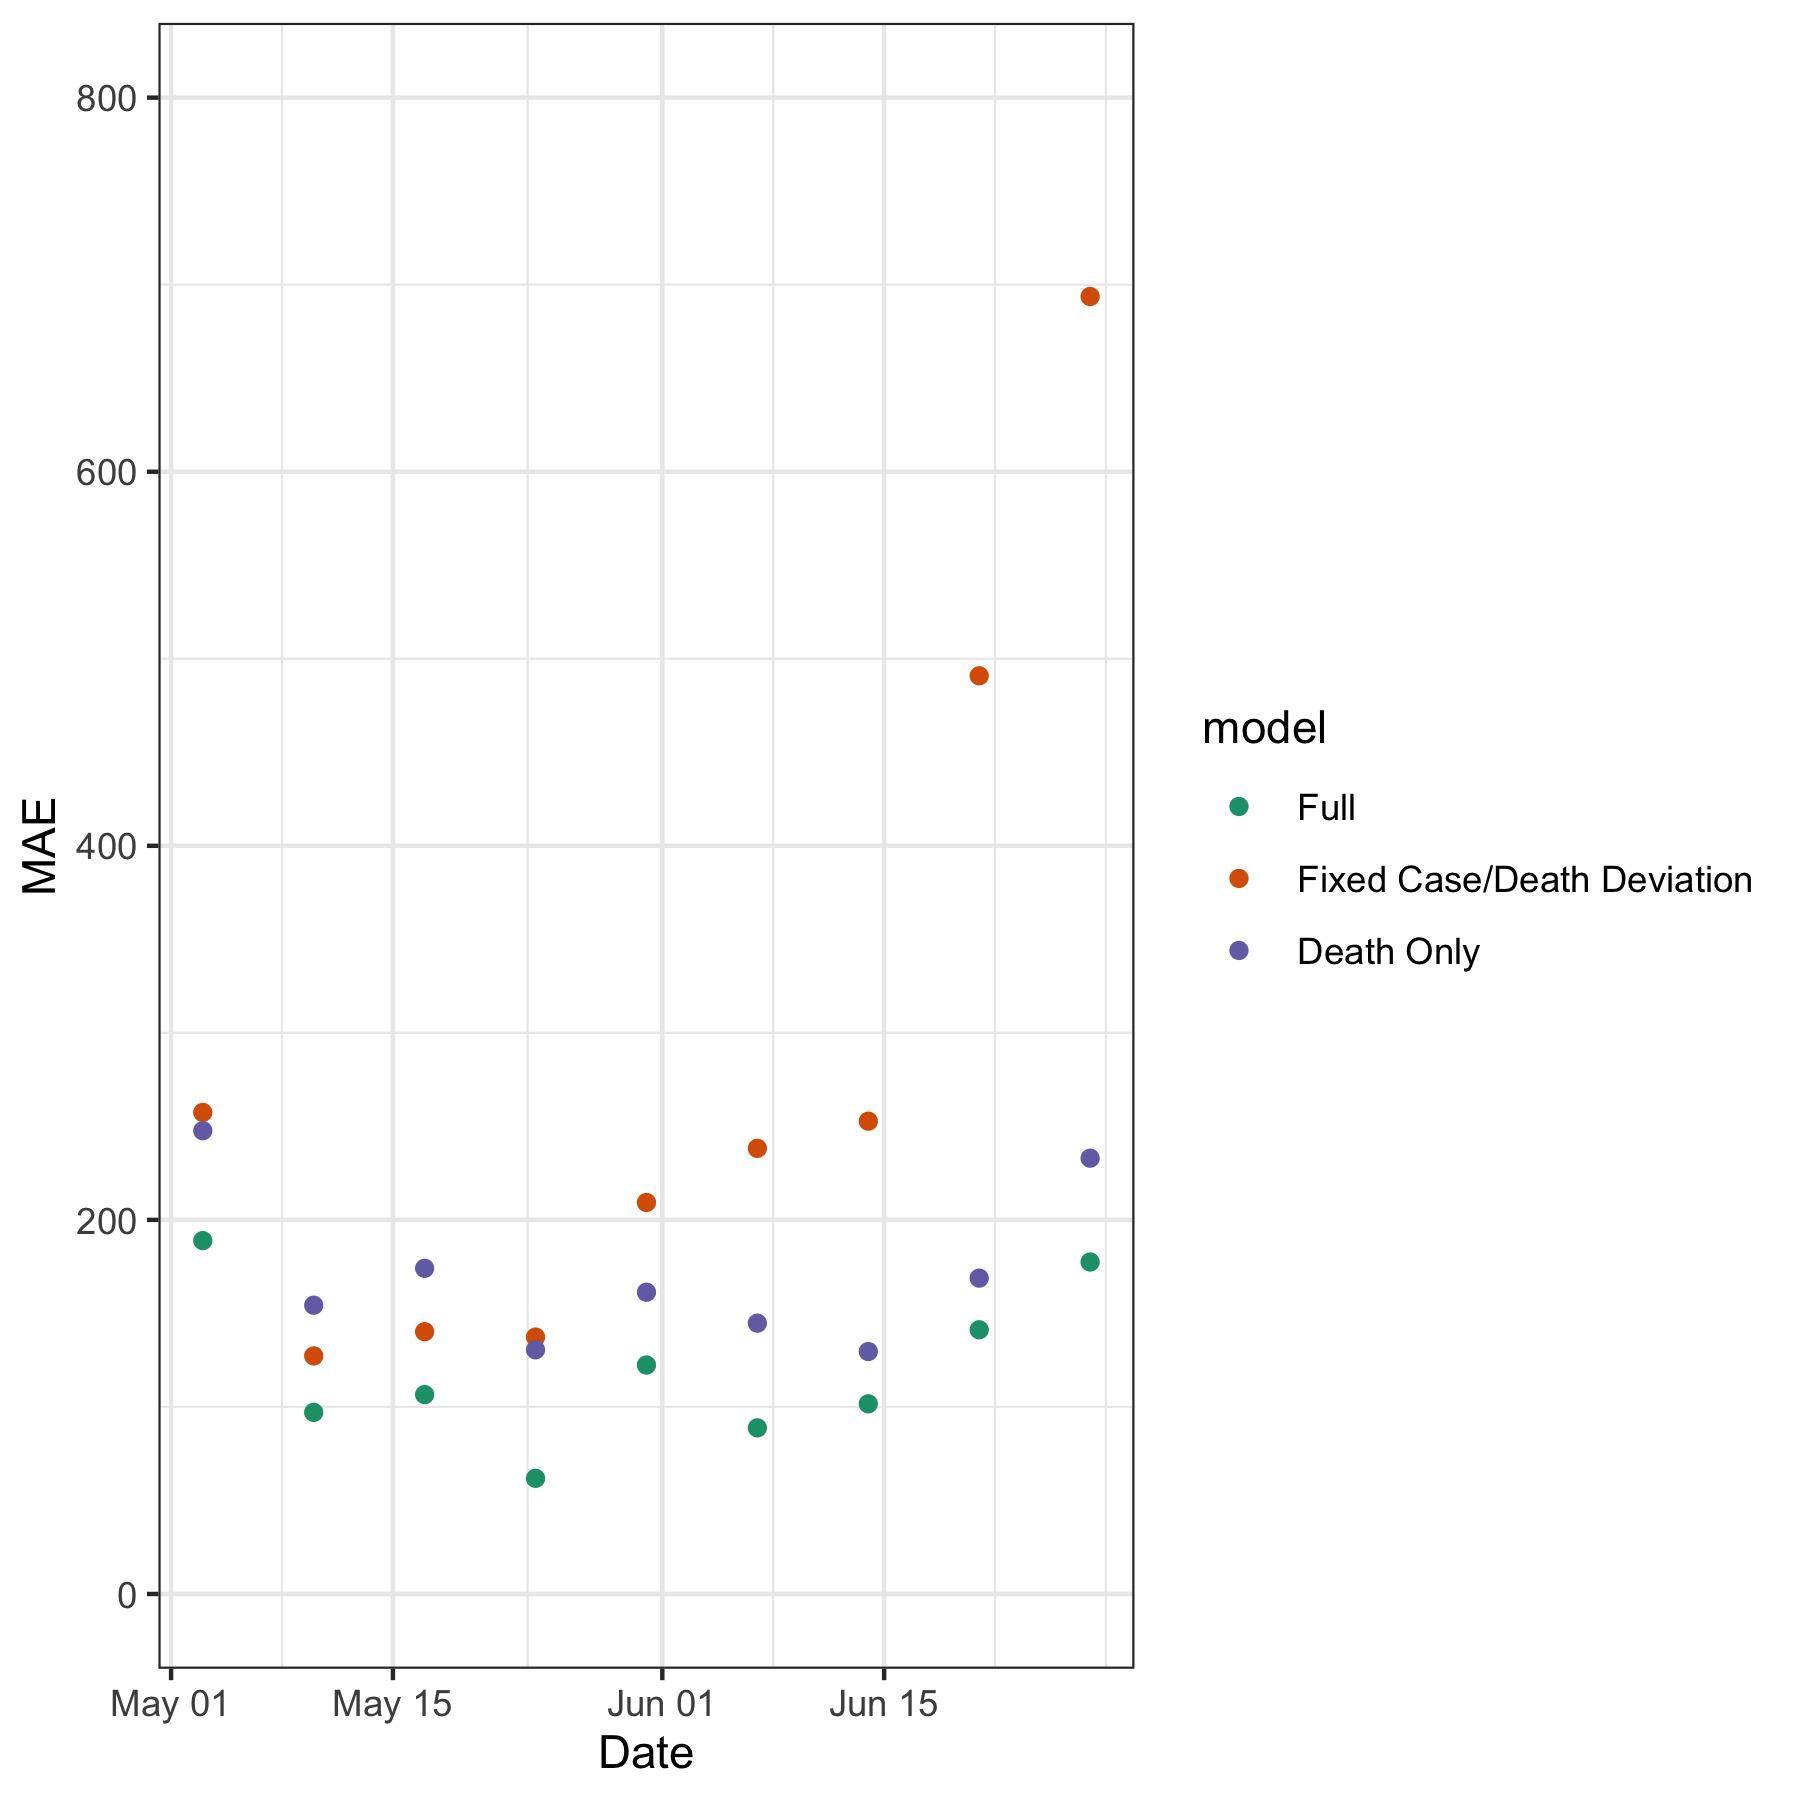
\includegraphics[scale=.15]{ablation_4.png}
    \caption{4 week ahead. }
\end{subfigure}

\caption{Ablation test MAE broken down by forecast week and target. We can see that MechBayes Full performs better than MechBayes Fixed Case/Death Deviation and MechBayes Only death in almost all breakdowns. We can also see that the improvement becomes more pronounced at larger horizons, suggesting that MechBayes Full is a better longer term forecasting model.  }
\label{fig:ablation}
\end{figure}




\section{Discussion}

MechBayes is a fast, fully Bayesian compartmental model capable of accounting for real-world data challenges during a pandemic.  This model produced consistently accurate real-time forecasts over the course of 3 months, and was ranked as one of the top 3 of 11 models on an independent scoreboard of COVID-19 forecast models \cite{yyg}. Our experiments led us to the following conclusions about the performance of this model and the underlying methodology.

\begin{itemize}

\item \textbf{MechBayes is accurate when compared to a baseline model}. As Figure \ref{fig:covidhub} shows, MechBayes improved relative to the baseline model when broken down by timezero and target. The results are more pronounced when breaking down by target, where the boxplots (95\%) are almost completely separated. These results are statistically significant for 1-4 weeks ahead, with larger improvements at later horizons, suggesting that the biggest improvements from MechByes over the baseline model comes in longer term forecasting. Additionally, as seen in Figure \ref{fig:covidhub_region_results} , the biggest gains in performance in MAE occur in regions with the largest total deaths counts. This is a desirable feature of a pandemic forecasting model. 

\item \textbf{MechBayes is probabilistically well-calibrated compared with the baseline model}. As we can see from Figure \ref{fig:covidhub} (B,D), the coverage probability of MechBayes is much closer to 95\%. When averaging over target, region, and timezero the coverage probability is 94.6\%. This suggests that MechBayes is very well calibrated at the 95\% level. The two sources of uncertainty in MechBayes come from the distribution over the differential equation parameters and the observation noise. The model is able to learn reasonable estimates of these variance parameters to produce well calibrated results. 


\item \textbf{Adding case data when predicting deaths is helpful but only when accounting for data quality issues}. Our ablation tests (Figure \ref{fig:ablation}) clearly shows that time-varying case and death deviation model is a key feature in the model for reducing MAE of forecasts. The "Full" model that both incorporates incident cases into the model likelihood and allows for a flexible deviation between cases and deaths is consistently more accurate than a model that does not account for cases at all ("Death Only" model) and a model that does account for cases but does not account for a time-varying deviation between cases and deaths.

%As we can see in Figure \ref{fig:model_details}, the model relies on this parameter heavily, setting the case and death deviation model at around 15\% at the start of the pandemic in March, to nearly 80\% by August 1st 2020. There is remarkable similarity between the increase across geographical locations as well, suggesting (as testing data reflects) an overall increase in the number of detected cases across the U.S. Adjusting for case data quality also requires a QA process, where data dumps are redistributed across a specific time-window. This avoids the situation where MechBayes interprets data dumps as a drastic change in disease dynamics. This is visible in Figure \ref{fig:model_details}, where the time-varying case and death deviation model in New Jersey follows the typical trend of other states, until the data dump, where the case and death deviation model dips significantly down.



\item \textbf{MechBayes is biased high}. We can see from Figure \ref{fig:results_discussion} that MechBayes was biased high with respect to the median forecast. We suspect this is due to the inherent exponential growth of an SEIR model when the number of susceptibles is small. Since overall prevalence in any state is well below the number needed to reach herd immunity, when the model sees an increase in cases it treats this as exponential growth, which translates into exponential growth in deaths. However, in the recent forecasts the bias is consistently lower than the COVID-19 Forecast Hub baseline model. Note the extreme low bias in the first submission is due to the omission of the U.S. in the submission. \textbf{is this true} 

\item \textbf{Most epidemiological parameters are unidentifiable from the data}. MechBayes requires relatively informative priors on $\sigma$, $\gamma$, $\rho$ and $\lambda$. These parameters reflect the biology of the disease, from latent incubation period to average time from symptom onset to death. Since the data used to fit MechBayes is only a time series of confirmed cases and deaths, these parameters are simply not identifiable from the data. However, using a Bayesian framework we can simultaneously set priors based on the literature and allow for small deviations from the prior due to variations across states. 




\item \textbf{Allowing for time-varying transmissibility is necessary to non-parametrically capture the effect of  interventions}. Our ablation test explicitly did not include a model that fixed $\beta$ across time. This is because the model would not converge without the flexibility to capture changes in transmission. While non-parametrically modeling interventions is appealing from a forecasting perspective, it does modify the philosophy behind compartmental modeling. By including such a flexible parameter, we may view MechBayes as simply a random-walk model, with a set of epidemiological parameters transforming that random-walk in an almost deterministic way to match both cases and deaths. For instance, if the variance of the random walk $\sigma_{\beta}^2$ was allowed to be arbitrarily large, then $\beta(t)$ could vary enough to match the data exactly. This would clearly attribute reporting issues as true changes in transmissibility. Bypassing the epidemiological interpretation that compartmental models provide. 

\end{itemize}




\begin{figure}
\centering
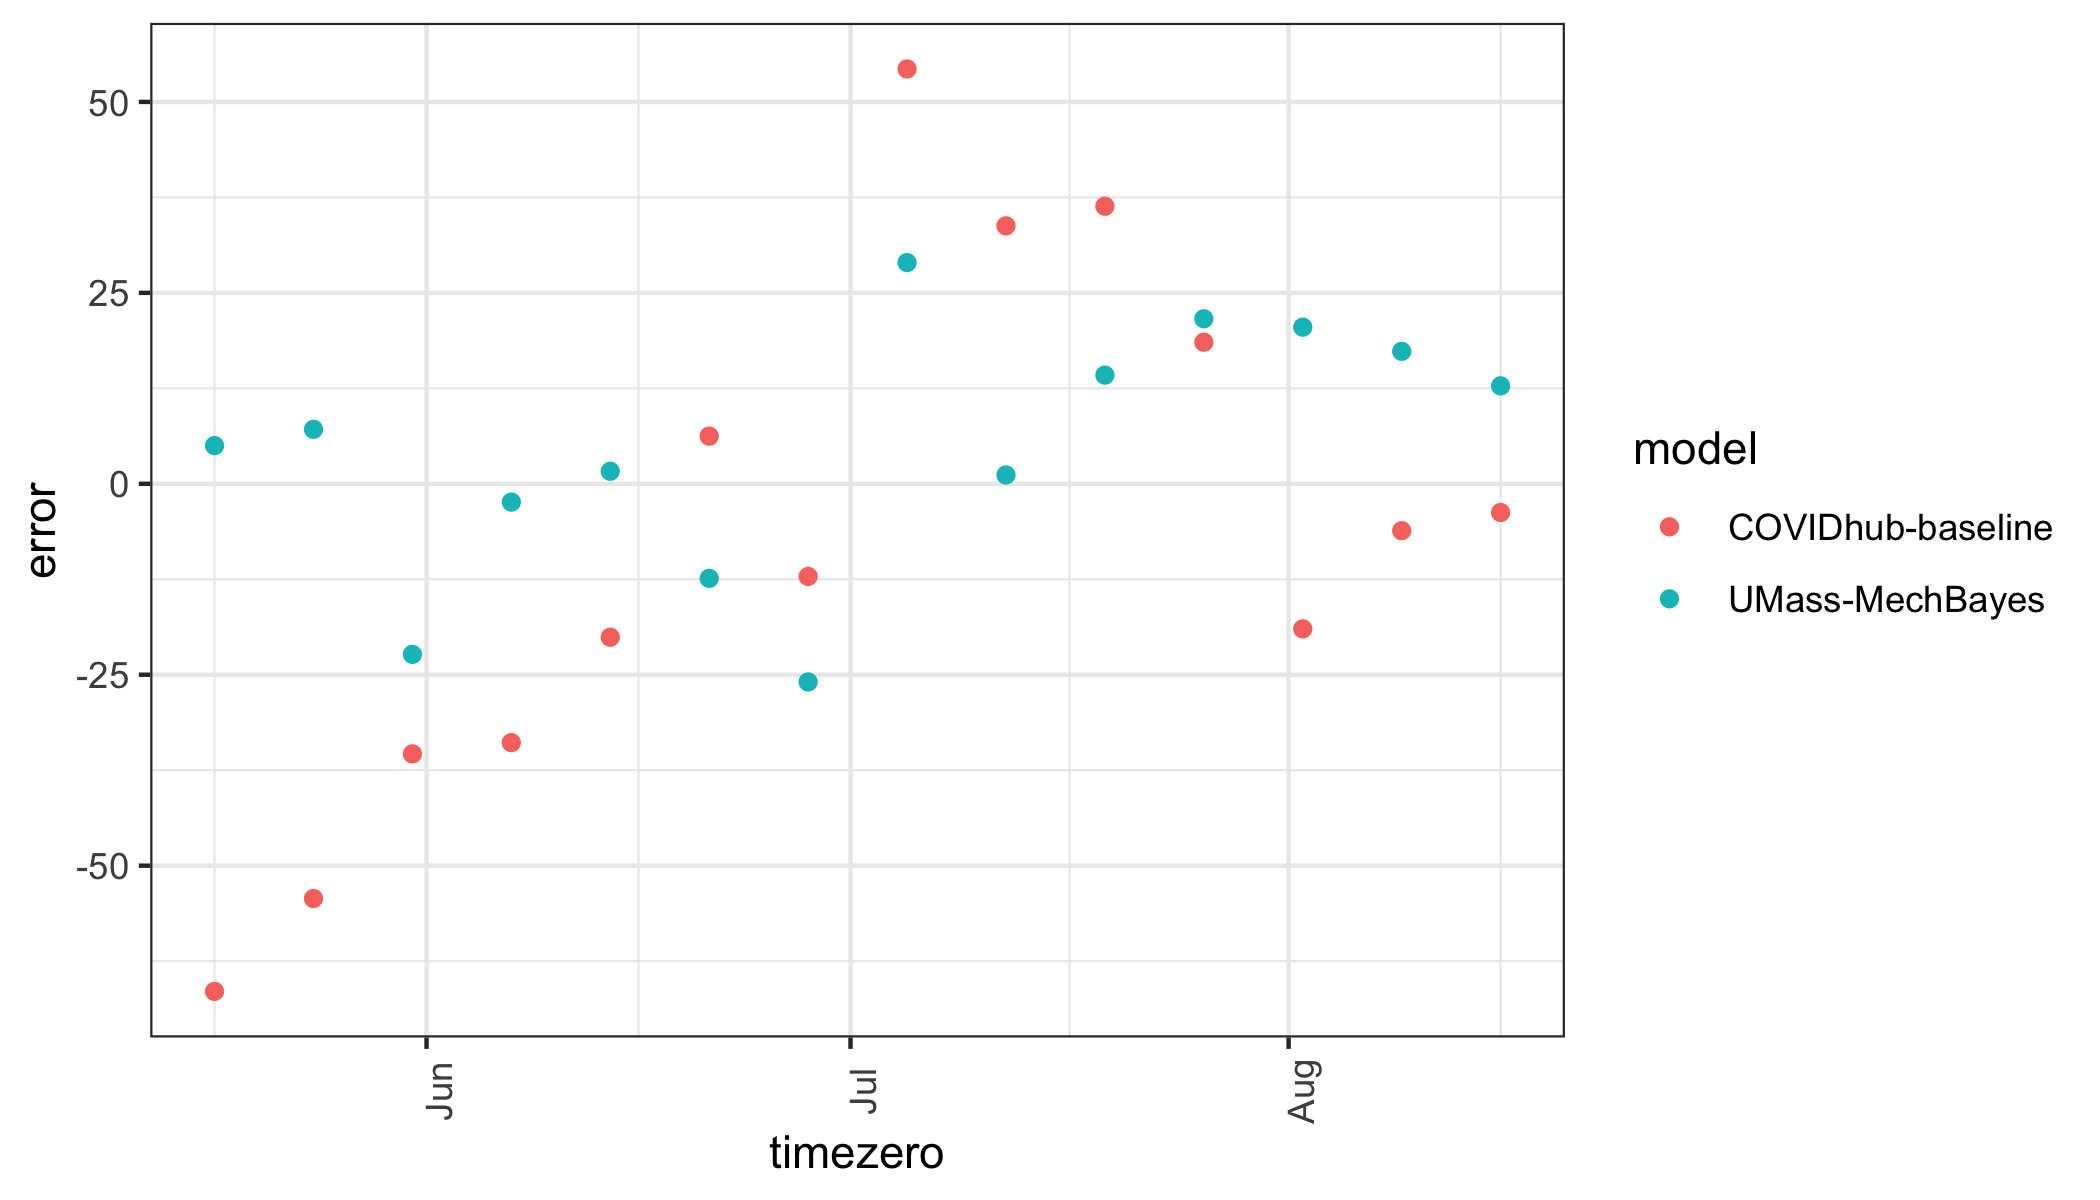
\includegraphics[scale=.15]{bias_by_timezero.png}
\caption{Bias of MechBayes and COVID-Baseline as a function of time.  }
\label{fig:results_discussion}
\end{figure}



\section{Conclusion}

We have seen that MechBayes is a powerful Bayesian compartmental model that can capture the real-world complexities of forecasting during a pandemic. Through real-time and retrospective evaluation, we have demonstrated the success of MechBayes in forecasting COVID-19. The model is able to improve over a naive baseline model as well as a naive compartmental model. Allowing for time-varying interventions and case and death deviation model is a necessary model component during a real-time pandemic forecasting effort. 

While we chose an exponential random walk on $\beta(t)$ there are many other choices for flexible non-parametric modeling of transmissibility. Further work might consider a spline model, or a Gaussian process, or semi-parametric models capable of taking intervention dates as covariates. 

However, using relatively simple non-parametric methods we were able to beat the COVID-19 Forecast Hub baseline model in both point and probabilistic forecast evaluations. Our ablation tests show that extending the basic SEIR compartmental to real-world pandemic challenges improves forecasting accuracy. 


\newpage

\section{Appendix}
\subsection{A1}
\subsection{Seeding Epidemic}
Due to the under-reporting of cases, we cannot use the observed data to seed the epidemic. We instead allow the model to find the initial state values for all compartments except the number of susceptible people, which we take as the population size of the geographic region minus the sum of the initial values for the other compartments to enforce the constraint that the entire system size sums to the population size. We do this by assigning uniform probability to all initial states where the number of people in any given compartment at time zero does not exceed 2\% of the total population. This is a highly conservative estimate for the number of infected, exposed, dead and recovered people at the start of the epidemic which is most likely much lower than 2\% of the population. 

\begin{align*}
 E_0 &\sim \Unif(0, 0.02 N) \\
I_0 &\sim \Unif(0, 0.02 N) \\
  D_{1_0} &\sim \Unif(0, 0.02 N) \\
   D_{2_0} &\sim \Unif(0, 0.02 N) \\   
   R_{0} &\sim \Unif(0, 0.02 N) \\   
\end{align*}

This allows us to initialize the process model:
 \begin{equation} 
 X(0) = (S(0), E(0), I(0), R(0), D_1(0), D_2(0), C(0)) = (N-E_0-I_0-D_{1_0}-D_{2_0},E_0,I_0, R_0, D_{1_0}, D_{2_0}, I_0)
 \end{equation}
%
% \begin{itemize}
% \item Because of case and death deviation model we cannot seed using initial reported data, since this is an underestimate
% \item Put priors on initial seed
%  \end{itemize}
  
  \subsection{Priors}
We also place the following priors on the transition parameters: 
\begin{align*}
\sigma &\sim \Gamma(5, 5 \hat{d}_E)\\
\gamma & \sim \Gamma(7, 7 \hat{d}_I) \\
\beta(0) &\sim \Gamma(1, \hat{d}_I/\hat{R}) \\
    \rho &\sim \Beta(10, 90)\\ 
\lambda &\sim \Gamma(10, 100)
\end{align*}
 Our prior on rate for leaving the exposed compartment $\sigma$ satisfies $\E[\sigma] = 1/\hat{d}_E$, where $\hat{d}_E$ is an initial guess of the duration of the latent period. Currently, we assume $\hat{d}_E = 4.0$ based on published estimates (shortened slightly to account for possible infectiousness prior to developing symptoms) \cite{midas}.
 %
 Our prior on the rate for leaving the infectious compartment $\gamma$ satisfies $\E[\gamma] = 1/\hat{d}_I$, where $\hat{d}_I$ is an initial guess for the duration of infectiousness. The current setting is $\hat{d}_I = 2.0$ to model the likely isolation of individuals after symptom onset \cite{heffner2020emotional}. 
Our prior on the initial transmission rate is derived from the relationship between the basic reproductive number $R(0)$ and the length of the infectious period: $R(0) = \beta(0)/\gamma = \beta(0)\times \hat{d}_I$. Therefore, we set our prior on the initial transmission rate to satisfy $\E[\beta(0)] = \hat{R}/\hat{d}_I$ where $\hat{R} = 3.0$ is an initial guess for $R(0)$ and $\hat{d}_I = 2.0$, as described above. 
%%
Our prior on the fatality rate $\rho$ satisfies $\E[\rho] = 0.1$ with 90\% probability of being between \[0.06,.14\].
Finally, our prior on the rate at which dying patients succumb  satisfies $\lambda$ $\E[\lambda] = 0.1$ with shape 10 corresponding to roughly 10 days in the $D_{1}$ compartment.


%% End of body
%%%%%%%%%%%%%%%%%%%%%%%%%%%%%%%%%%%%%%%%%%%%%%%%%%%%%%%%%%%%%%%%%%%%%%%%%%%%%%%

\appendix
\chapter{THE FIRST APPENDIX TITLE}
...
\chapter{THE SECOND APPENDIX TITLE}
...

%%
%% Beginning of back matter
\backmatter  %% <--- mandatory

%%
%% We don't support endnotes

%%
%% A bibliography is required.
\interlinepenalty=10000  % prevent split bibliography entries
\bibliographystyle{umassthesis}
\bibliography{bib}
\end{document}

%%% Local Variables: 
%%% mode: latex
%%% TeX-master: t
%%% End: 
